% PLEASE USE THIS FILE AS A TEMPLATE
%DIF LATEXDIFF DIFFERENCE FILE
%DIF DEL /tmp/orig/texsupport.iospress-sw-master/main.tex   Tue Jun  9 12:58:48 2026
%DIF ADD main.tex                                           Sun Jun 14 14:24:16 2026
% Check file iosart2x.tex for more examples

% add. options: [seceqn,secthm,crcready]
\documentclass[sw]{iosart2x}
%\usepackage{dcolumn}

\usepackage{graphicx}
\usepackage{listings}
\usepackage{xcolor}
% \usepackage{caption}  % To use \captionof outside of floats

\definecolor{keywordcolor}{RGB}{255,127,0} % Custom color for keywords
\definecolor{lightgray}{rgb}{0.95, 0.95, 0.95} % Define a very light gray color

\lstset{
    language=Python,
    basicstyle=\ttfamily\scriptsize, % Smaller font size
    keywordstyle=\color{keywordcolor}\bfseries,
    commentstyle=\color{gray},
    stringstyle=\color{blue},
    showstringspaces=false,
    frame=single,
    breaklines=true,
    tabsize=4,
    numbers=left, % Disable line numbers in the margin
    backgroundcolor=\color{lightgray}, % Light gray background color
}

%%%%%%%%%%% Put your definitions here

%%%%%%%%%%% End of definitions


\pubyear{0000}
\volume{0}
\firstpage{1}
\lastpage{1}
%DIF PREAMBLE EXTENSION ADDED BY LATEXDIFF
%DIF UNDERLINE PREAMBLE %DIF PREAMBLE
\RequirePackage[normalem]{ulem} %DIF PREAMBLE
\RequirePackage{color}\definecolor{RED}{rgb}{1,0,0}\definecolor{BLUE}{rgb}{0,0,1} %DIF PREAMBLE
\providecommand{\DIFadd}[1]{{\protect\color{blue}\uwave{#1}}} %DIF PREAMBLE
\providecommand{\DIFdel}[1]{{\protect\color{red}\sout{#1}}} %DIF PREAMBLE
%DIF SAFE PREAMBLE %DIF PREAMBLE
\providecommand{\DIFaddbegin}{} %DIF PREAMBLE
\providecommand{\DIFaddend}{} %DIF PREAMBLE
\providecommand{\DIFdelbegin}{} %DIF PREAMBLE
\providecommand{\DIFdelend}{} %DIF PREAMBLE
\providecommand{\DIFmodbegin}{} %DIF PREAMBLE
\providecommand{\DIFmodend}{} %DIF PREAMBLE
%DIF FLOATSAFE PREAMBLE %DIF PREAMBLE
\providecommand{\DIFaddFL}[1]{\DIFadd{#1}} %DIF PREAMBLE
\providecommand{\DIFdelFL}[1]{\DIFdel{#1}} %DIF PREAMBLE
\providecommand{\DIFaddbeginFL}{} %DIF PREAMBLE
\providecommand{\DIFaddendFL}{} %DIF PREAMBLE
\providecommand{\DIFdelbeginFL}{} %DIF PREAMBLE
\providecommand{\DIFdelendFL}{} %DIF PREAMBLE
\providecommand{\DIFscaledelfig}{0.5}
%DIF HIGHLIGHTGRAPHICS PREAMBLE %DIF PREAMBLE
\RequirePackage{settobox} %DIF PREAMBLE
\RequirePackage{letltxmacro} %DIF PREAMBLE
\newsavebox{\DIFdelgraphicsbox} %DIF PREAMBLE
\newlength{\DIFdelgraphicswidth} %DIF PREAMBLE
\newlength{\DIFdelgraphicsheight} %DIF PREAMBLE
% store original definition of \includegraphics %DIF PREAMBLE
\LetLtxMacro{\DIFOincludegraphics}{\includegraphics} %DIF PREAMBLE
\providecommand{\DIFaddincludegraphics}[2][]{{\color{blue}\fbox{\DIFOincludegraphics[#1]{#2}}}} %DIF PREAMBLE
\providecommand{\DIFdelincludegraphics}[2][]{% %DIF PREAMBLE
\sbox{\DIFdelgraphicsbox}{\DIFOincludegraphics[#1]{#2}}% %DIF PREAMBLE
\settoboxwidth{\DIFdelgraphicswidth}{\DIFdelgraphicsbox} %DIF PREAMBLE
\settoboxtotalheight{\DIFdelgraphicsheight}{\DIFdelgraphicsbox} %DIF PREAMBLE
\scalebox{\DIFscaledelfig}{% %DIF PREAMBLE
\parbox[b]{\DIFdelgraphicswidth}{\usebox{\DIFdelgraphicsbox}\\[-\baselineskip] \rule{\DIFdelgraphicswidth}{0em}}\llap{\resizebox{\DIFdelgraphicswidth}{\DIFdelgraphicsheight}{% %DIF PREAMBLE
\setlength{\unitlength}{\DIFdelgraphicswidth}% %DIF PREAMBLE
\begin{picture}(1,1)% %DIF PREAMBLE
\thicklines\linethickness{2pt} %DIF PREAMBLE
{\color[rgb]{1,0,0}\put(0,0){\framebox(1,1){}}}% %DIF PREAMBLE
{\color[rgb]{1,0,0}\put(0,0){\line( 1,1){1}}}% %DIF PREAMBLE
{\color[rgb]{1,0,0}\put(0,1){\line(1,-1){1}}}% %DIF PREAMBLE
\end{picture}% %DIF PREAMBLE
}\hspace*{3pt}}} %DIF PREAMBLE
} %DIF PREAMBLE
\LetLtxMacro{\DIFOaddbegin}{\DIFaddbegin} %DIF PREAMBLE
\LetLtxMacro{\DIFOaddend}{\DIFaddend} %DIF PREAMBLE
\LetLtxMacro{\DIFOdelbegin}{\DIFdelbegin} %DIF PREAMBLE
\LetLtxMacro{\DIFOdelend}{\DIFdelend} %DIF PREAMBLE
\DeclareRobustCommand{\DIFaddbegin}{\DIFOaddbegin \let\includegraphics\DIFaddincludegraphics} %DIF PREAMBLE
\DeclareRobustCommand{\DIFaddend}{\DIFOaddend \let\includegraphics\DIFOincludegraphics} %DIF PREAMBLE
\DeclareRobustCommand{\DIFdelbegin}{\DIFOdelbegin \let\includegraphics\DIFdelincludegraphics} %DIF PREAMBLE
\DeclareRobustCommand{\DIFdelend}{\DIFOaddend \let\includegraphics\DIFOincludegraphics} %DIF PREAMBLE
\LetLtxMacro{\DIFOaddbeginFL}{\DIFaddbeginFL} %DIF PREAMBLE
\LetLtxMacro{\DIFOaddendFL}{\DIFaddendFL} %DIF PREAMBLE
\LetLtxMacro{\DIFOdelbeginFL}{\DIFdelbeginFL} %DIF PREAMBLE
\LetLtxMacro{\DIFOdelendFL}{\DIFdelendFL} %DIF PREAMBLE
\DeclareRobustCommand{\DIFaddbeginFL}{\DIFOaddbeginFL \let\includegraphics\DIFaddincludegraphics} %DIF PREAMBLE
\DeclareRobustCommand{\DIFaddendFL}{\DIFOaddendFL \let\includegraphics\DIFOincludegraphics} %DIF PREAMBLE
\DeclareRobustCommand{\DIFdelbeginFL}{\DIFOdelbeginFL \let\includegraphics\DIFdelincludegraphics} %DIF PREAMBLE
\DeclareRobustCommand{\DIFdelendFL}{\DIFOaddendFL \let\includegraphics\DIFOincludegraphics} %DIF PREAMBLE
%DIF COLORLISTINGS PREAMBLE %DIF PREAMBLE
\RequirePackage{listings} %DIF PREAMBLE
\RequirePackage{color} %DIF PREAMBLE
\lstdefinelanguage{DIFcode}{ %DIF PREAMBLE
%DIF DIFCODE_UNDERLINE %DIF PREAMBLE
  moredelim=[il][\color{red}\sout]{\%DIF\ <\ }, %DIF PREAMBLE
  moredelim=[il][\color{blue}\uwave]{\%DIF\ >\ } %DIF PREAMBLE
} %DIF PREAMBLE
\lstdefinestyle{DIFverbatimstyle}{ %DIF PREAMBLE
	language=DIFcode, %DIF PREAMBLE
	basicstyle=\ttfamily, %DIF PREAMBLE
	columns=fullflexible, %DIF PREAMBLE
	keepspaces=true %DIF PREAMBLE
} %DIF PREAMBLE
\lstnewenvironment{DIFverbatim}[1][]{\lstset{style=DIFverbatimstyle}}{} %DIF PREAMBLE
\lstnewenvironment{DIFverbatim*}[1][]{\lstset{style=DIFverbatimstyle,showspaces=true}}{} %DIF PREAMBLE
\lstset{extendedchars=\true,inputencoding=utf8}

%DIF END PREAMBLE EXTENSION ADDED BY LATEXDIFF

\begin{document}

\begin{frontmatter}

%\pretitle{}
\title{Knowledge graph usage metadata: Insights from SPARQL log analysis
}
\runtitle{Knowledge graph usage metadata: Insights from SPARQL log analysis}
%\subtitle{}

% For one author:
%\author{\inits{N.}\fnms{Name1} \snm{Surname1}\ead[label=e1]{first@somewhere.com}}
%\address{Department first, \orgname{University or Company name},
%Abbreviate US states, \cny{Country}\printead[presep={\\}]{e1}}

% Two or more authors:
\begin{aug}
\author[A,B]{\inits{M.}\fnms{Maryam} \snm{Mohammadi}\ead[label=e1]{m.mohammadi@maastrichtuniversity.nl}%
\thanks{Corresponding author. \printead{e1}.}}

\author[A,B]{\inits{Ch.}\fnms{Chang} \snm{sun}\ead[label=e2]{chang.sun@maastrichtuniversity.nl}}

\author[A,B]{\inits{R.}\fnms{Remzi} \snm{Celebi}\ead[label=e3]{remzi.celebi@maastrichtuniversity.nl}}

\author[A,B,C]{\inits{ch.}\fnms{Christopher} \snm{Brewster}\ead[label=e4]{christopher.brewster@maastrichtuniversity.nl}}

\author[A,B]{\inits{M.}\fnms{Michel} \snm{Dumontier}\ead[label=e5]{michel.dumontier@maastrichtuniversity.nl}}

\address[A]{Institute of Data Science, Faculty of Science and Engineering, \orgname{Maastricht University}, \cny{The Netherlands}}
\address[B]{Department of Advanced Computing Sciences, Faculty of Science and Engineering, \orgname{Maastricht University}, \cny{The Netherlands}}

% \printead[presep={\\}]{e1,e2,e3,e4,e5}
% \address[]{\orgname{Institute of Data Science}, Maastricht University, Maastricht, 6229 EN \cny{The~Netherlands}}
\address[C]{Data Science Group,\orgname{TNO}, Soesterberg, \cny{The Netherlands}}

\end{aug}

%\begin{review}{editor}
%\reviewer{\fnms{First} \snm{Editor}\address{\orgname{University or Company name}, \cny{Country}}}
%\reviewer{\fnms{Second} \snm{Editor}\address{\orgname{First University or Company name}, \cny{Country}
%    and \orgname{Second University or Company name}, \cny{Country}}}
%\end{review}
%\begin{review}{solicited}
%\reviewer{\fnms{First} \snm{Solicited reviewer}\address{\orgname{University or Company name}, \cny{Country}}}
%\reviewer{\snm{anonymous reviewer}}
%\end{review}
%\begin{review}{open}
%\reviewer{\fnms{First} \snm{Open Reviewer}\address{\orgname{University or Company name}, \cny{Country}}}
%\end{review}

\begin{abstract}
Knowledge Graphs (KGs) are key technologies that enable enhanced understanding, knowledge representation, reasoning, and interpretation of complex data. The use of RDF KGs relies heavily on SPARQL queries for knowledge retrieval and manipulation. Analyzing SPARQL query logs can provide valuable insights into KG usage, revealing patterns in user behavior and interactions with the data. Prior studies have analyzed these logs in terms of their syntax and structure, but little is known about what parts of a KG are queried by users. This paper introduces content-based methods for analyzing KG usage, specifically examining the extent to which SPARQL queries cover the KG schema over defined time periods. We examine organic and robotic queries of Wikidata and Bio2RDF. \DIFdelbegin \DIFdel{Robotic queries have high schema coverage (60-97\%) , whereas organic queries exhibit lower schema coverage (14-21\% ).  }\DIFdelend \DIFaddbegin \DIFadd{Raw schema coverage is higher for robotic queries (60--97\%) than organic ones (14--21\%), but because the two query types differ greatly in volume, we control for sampling effort using individual-based rarefaction. This reveals a KG-dependent picture: on the compact, specialized Bio2RDF the broader robotic coverage is a genuine behavioral difference (robotic exercises $\sim$1.8$\times$ more of the schema at equal effort), whereas on the very large Wikidata the gap is largely a sampling-size artifact. Crucially, coverage is not directly comparable across the two: Bio2RDF has an OWL-style schema (classes with instances), whereas Wikidata is item-based, and we find that a large share of the items counted as queried ``classes'' --- about 30\% of those in human queries --- are in fact referenced as property values, not as classes. Comparing query demand against KG supply exposes a structural inversion: the most heavily instantiated Wikidata classes (e.g.\ geographic features) are rarely queried, while demand concentrates on a small, intuitive core. A third KG, DBpedia, confirms that this value-position effect tracks the modeling style (item-based vs.\ OWL) rather than KG size. }\DIFaddend Both datasets exhibit a sharp \DIFaddbegin \DIFadd{long-tailed }\DIFaddend decline in usage frequency\DIFdelbegin \DIFdel{indicating that a large set of schema elements is only infrequently queried. We perform statistical assessments to discover the trends and shifts in schema element usage across different }\DIFdelend \DIFaddbegin \DIFadd{, and we use statistical assessments --- validated across seven equal-length intervals --- to track shifts in schema-element usage across }\DIFaddend KG versions, query types, and log intervals. \DIFaddbegin \DIFadd{Finally, we show the usage metadata has concrete predictive value: a type-suggestion ranking learned from one year of logs captures most of the next year's query demand and substantially outperforms a ranking by KG content. }\DIFaddend Our work sheds light on \DIFdelbegin \DIFdel{KG usage, highlights frequently used schema elements as well as underused elements}\DIFdelend \DIFaddbegin \DIFadd{what is and is not queried in a KG}\DIFaddend , \DIFaddbegin \DIFadd{surfaces the mismatch between KG content and query demand, }\DIFaddend and provides guidance for \DIFdelbegin \DIFdel{improvements in }\DIFdelend documentation, schema design, and \DIFdelbegin \DIFdel{performance optimization}\DIFdelend \DIFaddbegin \DIFadd{the interpretation of usage metrics on item-based KGs}\DIFaddend .
\end{abstract}

\begin{keyword}
\kwd{Usage Metadata}
\kwd{RDF Knowledge Graph}
\kwd{SPARQL Query Logs}
\end{keyword}

\end{frontmatter}

%%%%%%%%%%% The article body starts:

\section{ Introduction }\label{s1}

Knowledge Graphs (KGs) are widely used as they are powerful representations of complex data. By organizing data into graph structures and ontologies, KGs facilitate semantic data integration, advanced search capabilities, and building neuro-symbolic  models \cite{abu2021domain,peng2023knowledge}. The Resource Description Framework (RDF) is a common model to implement a semantic KG. RDF KGs represent data as triples (subject-predicate-object), which allows for flexible and machine-readable descriptions of entities and their relationships. This standardized format is widely used for Linked Data on the Web \cite{ali2022survey}. SPARQL endpoints enable programmatic interaction with RDF KGs using the SPARQL language, and these interactions can be stored in a web server.  Analyzing the SPARQL query logs offers insight into what users are interested in and the manner in which they access desired information \cite{bielefeldt2018practical}, revealing patterns in computational demands, reliability, performance, user behavior, and data modeling decisions \cite{asprino2023your, mohammadi2022semi, Handschuh2010LearningFL,bonifati2017analytical,kaminski2018complexity, picalausa2011real,lorey2013detecting, raghuveer2012characterizing,rietveld2014man}. 

\DIFaddbegin \DIFadd{Throughout this paper we use three terms consistently. A }\emph{\DIFadd{type}} \DIFadd{(or class) is a resource used to classify instances, i.e., the object of a typing predicate such as }\texttt{\DIFadd{rdf:type}}\DIFadd{/}\texttt{\DIFadd{wdt:P31}} \DIFadd{or a subclass predicate such as }\texttt{\DIFadd{rdfs:subClassOf}}\DIFadd{/}\texttt{\DIFadd{wdt:P279}}\DIFadd{. A }\emph{\DIFadd{predicate}} \DIFadd{is the property in a triple $(s,p,o)$. An }\emph{\DIFadd{individual}} \DIFadd{is an instance, i.e., a non-schema resource (for example, a specific drug or person). We refer to the set of distinct types and predicates of a KG as its }\emph{\DIFadd{schema elements}}\DIFadd{.
}

\DIFaddend Previous studies on SPARQL query logs have primarily focused on the syntax and structure of these queries. These studies have analyzed keyword usage (e.g., count of SELECT, ASK, UNION, OPTIONAL) and query shapes (e.g., chain, tree, cycle), and their relation to evaluation complexity \cite{bonifati2020analytical, buil2015preliminary, saleem2015lsq,stadler2024lsq}. \DIFdelbegin \DIFdel{However, they often overlooked what users are interested in queries, i.e., the actual entities (types, relations, and instances) of the KG}\DIFdelend \DIFaddbegin \DIFadd{More recent work has begun to examine }\emph{\DIFadd{which}} \DIFadd{schema elements are queried: Bonifati et al. \mbox{%DIFAUXCMD
\cite{bonifati2019navigating} }\hskip0pt%DIFAUXCMD
analyze predicate usage in Wikidata query logs (including an interactive property sunburst), and Hammerer and Martens \mbox{%DIFAUXCMD
\cite{hammerer2025compendium} }\hskip0pt%DIFAUXCMD
catalog the Wikidata IRIs used for transitive (property-path) navigation}\DIFaddend . Asprino et al. \cite{asprino2023your} employed a content-centric approach to summarize query logs and identified query templates that qualitatively characterize user queries\DIFdelbegin \DIFdel{. These templates reveal }\DIFdelend \DIFaddbegin \DIFadd{, revealing }\DIFaddend patterns and contexts in which different types, relations, and instances are used. \DIFdelbegin \DIFdel{However, this work does not quantify the usage of each type, predicate, and individual, nor does it quantify overall KG content usage}\DIFdelend \DIFaddbegin \DIFadd{What is still missing, and what we provide, is a }\emph{\DIFadd{quantification}} \DIFadd{of how much of a KG's schema is covered by queries, of the usage frequency of each schema element, and of how this coverage shifts over time and between organic and robotic query types across two contrasting KGs}\DIFaddend .
This study explores ways to better understand the usage of KGs through the analysis of SPARQL query logs. We present novel methods to quantify schema (types and relations) usage, as well as to measure the frequency and the extent of that usage. Our research seeks to answer two main questions: (1) How can we quantify the usage of a KG? and (2) Do frequency distribution and ranking analyses of used KG elements reveal usage patterns over different log intervals or across organic (human-driven) and robotic (bot-driven) query types?

Previous work \cite{mohammadi2024analyzing} reported that most of the schema (types and relations) of the Bio2RDF KG was referred to within the SPARQL query logs over 30 months of queries. However, this work provided only a superficial view of user interaction with the KG, lacking deeper insights into the extent to which each schema element is accessed by users as well as differentiating between human and robotic interactions. 

In this study, we extend prior work \cite{mohammadi2024analyzing} to scrutinize the extent to which each schema element is included in user SPARQL queries while differentiating between organic and robotic queries from two KGs: Bio2RDF and Wikidata. The output of this analysis can be termed "usage metadata". The method produces novel usage metadata that offers practical insight into the extent to which KG is used by SPARQL users. Such information may be useful in understanding what users are querying in the KG and for targeted optimizations toward enhanced user engagement and operational efficiency. 
An innovative aspect of our approach is that it focuses on the triple patterns in SPARQL queries so as to focus on the types, relations, and individuals referred to in the queries. The main contributions of this paper, relative to preliminary work \cite{mohammadi2024analyzing}, are as follows:

\begin{itemize}
\item \textbf{\DIFdelbegin \DIFdel{Enhanced Schema Coverage Calculation Implementation:}\DIFdelend \DIFaddbegin \DIFadd{A robust pipeline for recovering schema elements from raw query logs.}\DIFaddend } \DIFdelbegin \DIFdel{Improved the accuracy and efficiency of SPARQL schema coverage computation by refining the query log triple pattern extraction and KG schema extraction.
}%DIFDELCMD < 

%DIFDELCMD < \item %%%
\item%DIFAUXCMD
\textbf{\DIFdel{Comparing KG Usage in Human vs. Bot Queries:}} %DIFAUXCMD
\DIFdel{Separated organic (human-driven)and robotic (bot-driven) queries to explore how their usage of KG content differs}\DIFdelend \DIFaddbegin \DIFadd{Raw logged query strings are frequently unparseable (missing prefix declarations, URL-encoding, appended HTTP parameters). We describe a preprocessing pipeline (prefix injection, URL-decoding, parameter removal, placeholder substitution, and variable standardization) that makes the logged queries parseable and aligns the schema extracted from the query side with the schema extracted from the KG side over a consistent reference set of subgraphs (Sections~\ref{s3}.3--\ref{s3}.4)}\DIFaddend .

\item \textbf{\DIFdelbegin \DIFdel{Identified }\DIFdelend \DIFaddbegin \DIFadd{Identification }\DIFaddend and \DIFdelbegin \DIFdel{Analyzed Usage Patterns }\DIFdelend \DIFaddbegin \DIFadd{analysis of usage patterns }\DIFaddend in \DIFdelbegin \DIFdel{Query Logs: }\DIFdelend \DIFaddbegin \DIFadd{query logs.}\DIFaddend } \DIFdelbegin \DIFdel{Identified schema element usage patterns by computing }\DIFdelend \DIFaddbegin \DIFadd{We compute schema-element }\DIFaddend frequency distributions and \DIFdelbegin \DIFdel{conducted statistical assessments to evaluate consistency and track changes intheir }\DIFdelend \DIFaddbegin \DIFadd{conduct statistical assessments (Shapiro--Wilk, Wilcoxon signed-rank, Spearman's rank correlation) to evaluate the consistency of, and changes in, schema-element }\DIFaddend usage in both Wikidata and Bio2RDF across \DIFdelbegin \DIFdel{different }\DIFdelend KG versions, query type\DIFaddbegin \DIFadd{s}\DIFaddend  , and log intervals.

\item \textbf{\DIFdelbegin \DIFdel{Demonstrated Method Applicability to Additional Logs:}\DIFdelend \DIFaddbegin \DIFadd{A size-controlled comparison of organic vs.\ robotic coverage.}\DIFaddend } \DIFdelbegin \DIFdel{Applied the improved }\DIFdelend \DIFaddbegin \DIFadd{Because logs of different query types differ greatly in size, raw coverage differences can be sampling-size artifacts. We add an individual-based rarefaction analysis (and Chao1 richness estimation) that compares schema coverage at equal sampling effort, disentangling genuine behavioral differences from differences in query volume.
}

\item \textbf{\DIFadd{What ``schema coverage'' means for an item-based KG, and a content--demand mismatch analysis.}} \DIFadd{Our coverage metric was first designed for Bio2RDF, whose OWL-style schema has classes with instances. Extending the study to Wikidata exposed that this assumption does not transfer: Wikidata is item-based, and we show that a large fraction of the items counted as queried ``classes'' are actually referenced as property }\emph{\DIFadd{values}}\DIFadd{, not as classes. We separate class-position from value-position usage, and we compare query }\emph{\DIFadd{demand}} \DIFadd{against KG }\emph{\DIFadd{supply}} \DIFadd{(instances per class), revealing a structural inversion between what Wikidata contains and what users query. A third KG, DBpedia, confirms that this value-position inflation tracks the schema model (item-based vs.\ OWL-style) rather than KG size, while the content--demand inversion generalizes across both.
}

\item \textbf{\DIFadd{A forecasting demonstration of downstream utility.}} \DIFadd{We show that the usage metadata has concrete predictive value: a type-suggestion ranking learned from 2017 logs captures most of the 2018 query demand, and substantially outperforms a ranking by KG content (instances per class), which wastes its top suggestions on bulk-imported but unqueried classes (Section~\ref{sec:utility}).
}

\item \textbf{\DIFadd{Demonstrated applicability to additional logs.}} \DIFadd{We apply the }\DIFaddend methods to new intervals of Bio2RDF \DIFdelbegin \DIFdel{logs }\DIFdelend and Wikidata logs \DIFdelbegin \DIFdel{, showcasing broader applicability and validating the method's effectiveness across different datasets}\DIFdelend \DIFaddbegin \DIFadd{across two KGs of very different scale and style}\DIFaddend .
\end{itemize}
The \DIFaddbegin \DIFadd{organic/robotic distinction itself is not our contribution: it was introduced for Wikidata by Malyshev et al.\ and Bielefeldt et al.\ \mbox{%DIFAUXCMD
\cite{malyshev2018getting,bielefeldt2018practical}}\hskip0pt%DIFAUXCMD
, and the Wikidata logs we use are already partitioned accordingly. Our only addition on this point is to apply the same user-agent classification algorithm of \mbox{%DIFAUXCMD
\cite{bielefeldt2018practical} }\hskip0pt%DIFAUXCMD
to the Bio2RDF~2019 logs so that all analyses can be reported separately for organic and robotic queries on both KGs.
The }\DIFaddend usage metadata from the proposed methods includes multiple components: a percentage value quantifying KG's overall usage in terms of its schema elements, the usage frequency of each element, and how usage changes over different log intervals and across two query types (organic and robotic).

The remainder of the paper is organized as follows: Section 2 reviews state-of-the-art methods of SPARQL query log analysis. Section 3 describes the proposed method. Section 4 presents the results, Section 5 offers a discussion of the findings and potential future directions. Finally, Section 6 concludes with a summary.

\section{Related Work}\label{s2}

Query logs capture user interactions with a system, and their analysis may provide insight into both what users are interested in and how they approach obtaining those results.  Prior work has focused on SPARQL log dataset creation, distinguishing between human and robotic queries, and query log summarization.

\textbf{Query Log Datasets.}
Studies \cite{saleem2015lsq,stadler2024lsq} introduce the Linked SPARQL Queries Dataset (LSQ), a public, openly accessible dataset of SPARQL queries extracted from KG endpoints. LSQ facilitates reuse by addressing the issue of legal agreements that limit access to raw query logs. It standardizes the format of logs, making them accessible for analysis. In this study, we use the LSQ SPARQL endpoint to access the Bio2RDF and Wikidata logs.

\textbf{Organic vs. Robotic Queries.} Bielefeldt et al. \cite{bielefeldt2018practical,malyshev2018getting} introduced the concept of organic and robotic SPARQL queries. They proposed a method to partition \DIFdelbegin \DIFdel{a dataset of over 200 million SPARQL queriesfrom Wikidata }\DIFdelend \DIFaddbegin \DIFadd{the Wikidata query logs they studied (on the order of hundreds of millions of queries; the live Wikidata Query Service has since logged far more) }\DIFaddend into organic and robotic queries. Robotic queries are generated by software tools or bots, while organic queries are generated by humans using browsers. Organic queries reflect end-user behavior, robotic queries may not directly capture user needs but often address backend requirements (e.g., serving internal or analytical purposes) or support application development. By distinguishing these types, the authors identified patterns in human usage and noted that robotic traffic of Wikidata displayed high volatility and unpredictability. We classify Bio2RDF queries into organic and robotic using the method in \cite{malyshev2018getting} and analyze organic and robotic queries of Wikidata and Bio2RDF.

\textbf{Content-Centric Analysis.} Previous work by Asprino et al. \cite{asprino2023your} introduced a content-centric method to analyze LSQ logs. Their method, termed query log summarization, categorizes SPARQL queries into common templates based on their content. By examining the ten most executed templates for each log, they identified common usage patterns and the prevalence of queries originating from a single code source. They also explored template relationships, uncovering evidence that related templates often participate in common processes and are frequently executed by similar sets of hosts. Additionally, their study highlighted relationships between different queries across various logs, indicating a systematic, automated approach to data querying. This work provides qualitative insight into KG  usage but does not quantify the usage of the KG content.

\DIFaddbegin \DIFadd{Closest to our content focus, Bonifati et al. \mbox{%DIFAUXCMD
\cite{bonifati2019navigating} }\hskip0pt%DIFAUXCMD
quantify predicate usage in Wikidata query logs and Hammerer and Martens \mbox{%DIFAUXCMD
\cite{hammerer2025compendium} }\hskip0pt%DIFAUXCMD
enumerate the IRIs used in property-path (transitive) navigation. Our work complements these by quantifying coverage over the }\emph{\DIFadd{full}} \DIFadd{schema (both types and predicates), reporting it as a single coverage percentage per (log, KG-version) pair, and tracking how it shifts over time and between organic and robotic queries. }\DIFaddend Although existing studies are valuable for analyzing KG usage, they do not provide \DIFdelbegin \DIFdel{insights into }\DIFdelend \DIFaddbegin \DIFadd{a quantitative measure of }\DIFaddend the extent to which \DIFdelbegin \DIFdel{KG schema elements are }\DIFdelend \DIFaddbegin \DIFadd{the KG schema as a whole is }\DIFaddend queried by users. Identifying the usage patterns may help optimize the KG development by guiding efforts, such as maintenance, toward the most frequently used or queried elements. This improves user experience by ensuring high-demand data is easily accessible and reliable, and reduces costs by allocating resources more efficiently and potentially deprecating underused elements. This paper presents an approach for quantifying SPARQL schema coverage and analyzing KG content usage.

\section{Method }\label{s3}
The workflow comprises six main steps as illustrated in Figure \ref{fig:l1}, beginning with retrieving SPARQL logs and downloading KG versions that approximately align with query log periods. The second step involves extracting schema elements from the KG. Next, we clean the SPARQL logs (step 3) in preparation for extracting the schema elements used within these logs (step 4). The fifth step involves calculating the SPARQL schema coverage, to assess how well the queries in the logs represent the KG's schema. Finally, we perform various analyses to discover usage patterns. Details of each step are described in the following subsections. 

\begin{figure} 
    \centering
    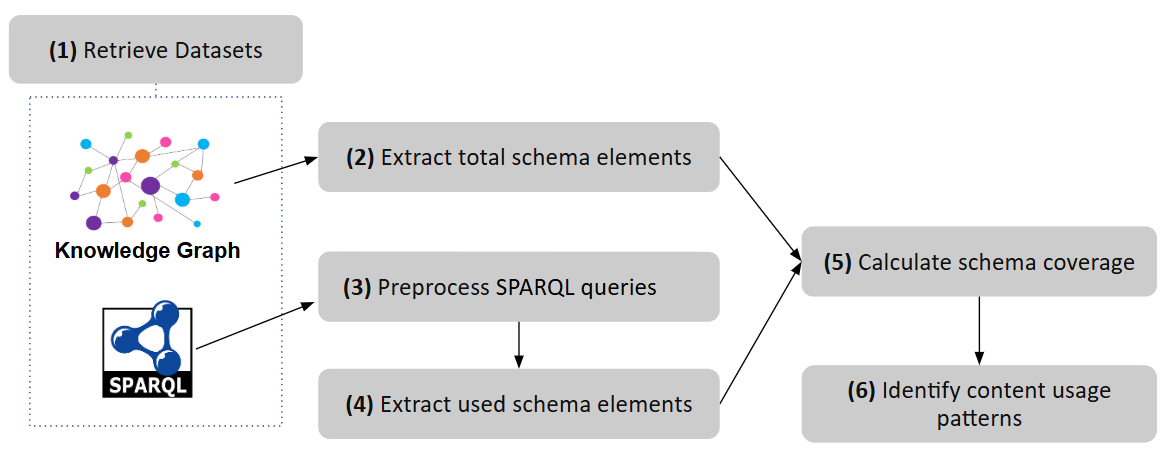
\includegraphics[width=0.8\textwidth]{image14.png} 
    \caption{Workflow of the proposed method }
    \label{fig:l1}
\end{figure}


\subsection{Datasets}

\textbf{RDF KGs.} Given that our analysis spans a period of Wikidata SPARQL query logs from 2017 to 2018, we downloaded a version of Wikidata from 2017 and 2018, as these are the closest versions available to the log period. This ensures maximum alignment of schema and query logs. We use both versions to investigate how the SPARQL schema coverage changes with the evolution of the Wikidata KG. We downloaded two versions of Wikidata from the Internet Archive\footnote{Wikidata version 2017: \url{https://archive.org/download/wikibase-wikidatawiki-20170821} and Wikidata version 2018: \url{https://archive.org/download/wikibase-wikidatawiki-20180205}}, and hosted them on Blazegraph on a local server. 

For Bio2RDF KG \cite{belleau2008bio2rdf}, the analysis covers two periods of SPARQL query logs: one beginning in 2013 and the other in 2019. However, due to the unavailability of datasets from these years, we instead use the current 2024 public endpoint\footnote{\url{https://Bio2RDF.org/sparql/}}.

\textbf{SPARQL Query Logs. }
The query logs are primarily retrieved from the Linked SPARQL Queries Dataset (LSQ) 2.0 endpoint\footnote{\url{https://lsq.data.dice-research.org/sparql}} using the query illustrated in Listing \ref{lst:SPARQL_query}. This query extracts the text and execution time of queries from 24 datasets in LSQ 2.0 \cite{stadler2024lsq}, including 23 Bio2RDF datasets and one Wikidata query dataset.
Furthermore, we downloaded Bio2RDF logs from Dumontier’s lab repository\footnote{\url{https://download.dumontierlab.com/Bio2RDF/logs/}} and Wikidata queries (all queries and organic queries for interval 1 and interval 7) from the International Center for Computational Logic\footnote{\url{https://iccl.inf.tu-dresden.de/web/Wikidata_SPARQL_Logs/en}}.

\DIFaddbegin \DIFadd{Among the many KGs available through LSQ, we selected Bio2RDF for two reasons. First, it is a domain-specific (life-sciences) KG with a compact, OWL-style schema, which contrasts sharply with the broad, general-purpose, and very large schema of Wikidata; comparing the two lets us study usage across two extremes of schema scale and design. Second, large Bio2RDF logs are available to us, including logs that retain user-agent information and therefore permit the organic/robotic split. The number of queries per dataset is substantial (ranging from $\sim$0.2 million to $\sim$81 million; full counts are reported in Tables~\ref{tab:1} and \ref{tab:2}), and we relate coverage to this sampling effort explicitly in Section~\ref{s4}.
}

\DIFadd{The interval boundaries are not chosen by us; they are inherited from the upstream releases. For Wikidata, intervals~1 and~7 are the two intervals of the ICCL/Dresden release that provide the organic/robotic partition together with sufficient volume, and they bracket an approximately one-year span (2017 vs.\ 2018) that aligns with the 2017 and 2018 KG dumps we host. For Bio2RDF, the 2013 and 2019 periods correspond to the two log dumps available (LSQ and the Dumontier-lab repository, respectively). Because these periods differ in length, all frequency analyses use }\emph{\DIFadd{time-normalized}} \DIFadd{counts (Section~\ref{sec:s61}), where one month is defined as a fixed 30-day period and a log's duration in months is computed as $(\text{end date}-\text{start date})/30$ days.
}


\DIFaddend \begin{center}
\begin{minipage}{0.8\textwidth}  % Adjust the width as needed
\begin{lstlisting}[label={lst:SPARQL_query},linewidth=\linewidth, caption={The templated SPARQL query against the LSQ SPARQL endpoint to retrieve SPARQL queries for selected datasets.}]
PREFIX lsqv: <http://lsq.aksw.org/vocab#>
PREFIX prov: <http://www.w3.org/ns/prov#>

SELECT DISTINCT ?text ?timeStamp

FROM <http://lsq.aksw.org/{dataset_name}>

WHERE {
    ?query  lsqv:text          ?text .
    ?query  lsqv:hasRemoteExec ?re .
    ?re     prov:atTime        ?timeStamp .
}
\end{lstlisting}
% \label{lst:SPARQL_query}
\end{minipage}
\end{center}


We implemented the method in \cite{bielefeldt2018practical, malyshev2018getting} to classify queries as organic or robotic based on the agent who executed the query. The Bio2RDF log2019 dataset includes user agent information, enabling us to generate the Bio2RDF organic and robotic log2019 subsets. The criteria used for classification are as follows:

\textbf{Organic:} If the user agent string contains indicators commonly associated with web browsers, such as "Mozilla," "Chrome," "Safari," "Firefox," "Edge," or "Opera," it was classified as organic. These are typically representative of human users.

\textbf{Robotic:} Entries \DIFdelbegin \DIFdel{lacking these browser indicators but containing terms like }\DIFdelend \DIFaddbegin \DIFadd{whose user agent lacks browser indicators were classified as robotic. In practice these agents carry terms such as }\DIFaddend "Apache," "HttpClient," "Crawler," "sparqlwrapper," \DIFdelbegin \DIFdel{or }\DIFdelend "python\DIFaddbegin \DIFadd{,}\DIFaddend " \DIFdelbegin \DIFdel{were classified as robotic,as these user agents are often }\DIFdelend \DIFaddbegin \DIFadd{or "Java," which are }\DIFaddend linked to automated scripts or bots\DIFaddbegin \DIFadd{; however, the operational rule is the complement of the organic test (any non-browser, non-empty agent), so that agents not matching a fixed keyword list are still treated as robotic rather than discarded}\DIFaddend .

\DIFaddbegin \textbf{\DIFadd{No agent:}} \DIFadd{A small number of entries carry no user-agent string and cannot be assigned to either class; they are excluded from the organic/robotic split.
}

\DIFaddend \subsection{Extracting Total Schema Elements}

In this study, the \DIFdelbegin \DIFdel{term KG schema refers to }\DIFdelend \DIFaddbegin \emph{\DIFadd{schema}} \DIFadd{of a KG is }\DIFaddend the set of \DIFdelbegin \DIFdel{types (or }\DIFdelend \DIFaddbegin \DIFadd{its distinct }\emph{\DIFadd{types}} \DIFadd{(}\DIFaddend classes) and \DIFdelbegin \DIFdel{predicates (or relationships) that define connections between instances of these types.
}\DIFdelend \DIFaddbegin \emph{\DIFadd{predicates}}\DIFadd{. A }\emph{\DIFadd{schema element}} \DIFadd{is one such type or predicate. A }\emph{\DIFadd{schema (type) pattern}} \DIFadd{is a triple pattern at the schema level, $(\text{type}_1,\ \text{predicate},\ \text{type}_2)$, i.e., an edge of the schema graph connecting instances of $\text{type}_1$ to instances of $\text{type}_2$ via $\text{predicate}$. We extract these schema elements directly from the data of each KG, because neither KG ships a single authoritative schema document that matches the deployed data.
}

\DIFaddend Listing~\ref{lst:l2} presents the pseudocode and queries used to extract the schema of a KG. The extraction process involves two main queries. Query\DIFdelbegin \DIFdel{\_}\DIFdelend \DIFaddbegin \DIFadd{~}\DIFaddend 1 (line 7 in Listing~\ref{lst:l2}) retrieves all types, while Query\DIFdelbegin \DIFdel{\_}\DIFdelend \DIFaddbegin \DIFadd{~}\DIFaddend 2 (line 13 in Listing~\ref{lst:l2}) extracts relationships between instances of different types. Using two optimized queries instead of a single complex query improved performance in large KGs, preventing timeout issues. \DIFdelbegin \DIFdel{However, }\DIFdelend \DIFaddbegin \DIFadd{For }\DIFaddend a few types, Query\DIFdelbegin \DIFdel{\_}\DIFdelend \DIFaddbegin \DIFadd{~}\DIFaddend 2 still encountered timeouts due to the high number of instances and relationships\DIFdelbegin \DIFdel{. In }\DIFdelend \DIFaddbegin \DIFadd{; in }\DIFaddend such cases, simplified queries were used to mitigate the issue.

For Bio2RDF and Wikidata, the properties used in these queries differ. In Bio2RDF, \DIFdelbegin \DIFdel{rdf:type and rdfs:subclassOf }\DIFdelend \DIFaddbegin \texttt{\DIFadd{rdf:type}} \DIFadd{and }\texttt{\DIFadd{rdfs:subClassOf}} \DIFaddend are used, whereas Wikidata employs \DIFdelbegin \DIFdel{wdt:P31 and wdt:P279 }\DIFdelend \DIFaddbegin \texttt{\DIFadd{wdt:P31}} \DIFadd{(}\emph{\DIFadd{instance of}}\DIFadd{) and }\texttt{\DIFadd{wdt:P279}} \DIFadd{(}\emph{\DIFadd{subclass of}}\DIFadd{) }\DIFaddend as their equivalents. Additionally, since Wikidata lacks subgraphs in its architecture, the \DIFdelbegin \DIFdel{"Graph" }\DIFdelend \DIFaddbegin \DIFadd{``Graph'' }\DIFaddend component is omitted from Query\DIFdelbegin \DIFdel{\_}\DIFdelend \DIFaddbegin \DIFadd{~}\DIFaddend 2 when applied to Wikidata. \DIFaddbegin \DIFadd{For Bio2RDF we additionally keep only IRIs that match the Bio2RDF vocabulary template }\url{http://Bio2RDF.org/DATASET_vocabulary:SCHEMA_ELEMENT} \DIFadd{(excluding the generic }\texttt{\DIFadd{:Resource}}\DIFadd{), which yields OWL-style class and property IRIs.
}\DIFaddend 

\DIFdelbegin \DIFdel{The schema }\DIFdelend \DIFaddbegin \paragraph{\textbf{\DIFadd{What counts as a ``class'' in Wikidata --- and how it is used.}}} \DIFadd{Bio2RDF follows a classical OWL-style design in which classes and properties have dedicated vocabulary IRIs and classes have instances, so its schema is unambiguous to extract. Wikidata is fundamentally different: its RDF model draws no formal class/instance separation. ``Classes'' are ordinary items, distinguished only by being used as the object of }\texttt{\DIFadd{wdt:P31}} \DIFadd{(}\emph{\DIFadd{instance of}}\DIFadd{) or }\texttt{\DIFadd{wdt:P279}} \DIFadd{(}\emph{\DIFadd{subclass of}}\DIFadd{); defining a Wikidata class is genuinely contested \mbox{%DIFAUXCMD
\cite{brasileiro2016applying,piscopo2018who,patelschneider2024class}}\hskip0pt%DIFAUXCMD
. Crucially --- and this is a measurement issue specific to item-based KGs --- the }\emph{\DIFadd{same}} \DIFadd{item is far more often referenced in queries as a property }\emph{\DIFadd{value}} \DIFadd{than as a class: e.g.\ }\texttt{\DIFadd{Q33999}} \DIFadd{(}\emph{\DIFadd{actor}}\DIFadd{) as the value of }\texttt{\DIFadd{P106}} \DIFadd{(}\emph{\DIFadd{occupation}}\DIFadd{), or }\texttt{\DIFadd{Q142}} \DIFadd{(}\emph{\DIFadd{France}}\DIFadd{) as the value of }\texttt{\DIFadd{P27}} \DIFadd{(}\emph{\DIFadd{country of citizenship}}\DIFadd{). A faithful usage analysis must therefore distinguish the }\emph{\DIFadd{position}} \DIFadd{in which an element is referenced. We call an entity reference }\emph{\DIFadd{class-position}} \DIFadd{when it is the object of }\texttt{\DIFadd{wdt:P31}}\DIFadd{/}\texttt{\DIFadd{wdt:P279}} \DIFadd{(or of a property path involving them, such as }\texttt{\DIFadd{wdt:P31/wdt:P279*}}\DIFadd{), and }\emph{\DIFadd{value-position}} \DIFadd{otherwise. Conflating the two --- as a naive ``type coverage'' does --- counts value usage as though it were schema usage; we therefore report the split (Section~\ref{sec:classvalue}). This distinction does not arise for Bio2RDF, whose vocabulary classes are not used as property values. We additionally distinguish }\emph{\DIFadd{instantiated}} \DIFadd{classes (objects of }\texttt{\DIFadd{wdt:P31}}\DIFadd{, $\geq 1$ instance) from purely hierarchical or uninstantiated items. These distinctions are central to interpreting the Wikidata coverage numbers and to the discussion of what ``schema coverage'' means for an item-based KG (Section~\ref{s5}).
}

\paragraph{\textbf{\DIFadd{Worked example.}}} \DIFadd{Consider the two example queries from the Wikidata Query Service. The first, }\texttt{\DIFadd{SELECT ?cat WHERE \{ ?cat wdt:P31 wd:Q146 \}}} \DIFadd{(house cats), references the predicate }\texttt{\DIFadd{P31}} \DIFadd{and the type }\texttt{\DIFadd{Q146}}\DIFadd{; both are extracted as used schema elements. The second, }\texttt{\DIFadd{?horse wdt:P31/wdt:P279* wd:Q726}} \DIFadd{(horses and their subclasses), references the predicates }\texttt{\DIFadd{P31}} \DIFadd{and }\texttt{\DIFadd{P279}} \DIFadd{and the type }\texttt{\DIFadd{Q726}}\DIFadd{; these three are extracted. Note that the }\texttt{\DIFadd{wdt:P279*}} \DIFadd{closure means the query also retrieves subclasses of horse (e.g.\ }\emph{\DIFadd{racehorse}}\DIFadd{, }\texttt{\DIFadd{Q2442470}}\DIFadd{), but those subclass IRIs are }\emph{\DIFadd{not}} \DIFadd{written in the query text and are therefore not counted as explicitly referenced (we return to this distinction in Section~\ref{s3}.4 and Section~\ref{s5}).
}

\DIFadd{The schema }\DIFaddend for any Bio2RDF dataset follows a specific URL template: \url{http://Bio2RDF.org/DATASET_vocabulary:SCHEMA_ELEMENT}. Therefore, any URLs retrieved from query execution that do not adhere to this template are excluded from the final schema elements set.


\begin{center}
\begin{minipage}{0.76\textwidth} % Adjust width here (e.g., 0.9 for 90% of text width)
\begin{lstlisting}[label={lst:l2},caption={Pseudocode to extract KG schema. KG schema extraction is consist of two queries, Query 1 and Query 2.}]
for graph in the KG:
        for each property in ['type_property', 'subclass_property']:
            Execute Query_1 to get subject_types
            for each subject_type and property in ['type_property', 'subclass_property']:
                execute Query_2 
                
Query_1:
SELECT DISTINCT ?subject_type
    WHERE {
        GRAPH <{graph}> {
            ?s {property} ?subject_type . } }

Query_2:
SELECT DISTINCT subject_type ?p ?object_type
WHERE {
    GRAPH <{graph}> {
        ?s {property} {subject_type} .
        ?s ?p ?o .
        ?o {property} ?object_type .  }} 
                    
\end{lstlisting}
\end{minipage}
\end{center}

\subsection{Preprocessing SPARQL Queries}

We extract unique SPARQL queries \DIFdelbegin \DIFdel{based on their text }\DIFdelend and store them along with their respective \DIFdelbegin \DIFdel{counts. }\DIFdelend \DIFaddbegin \DIFadd{execution counts. Two queries are considered identical when their text is identical after collapsing runs of whitespace (spaces, tabs, and newlines) to a single space and trimming leading/trailing whitespace; we do not otherwise reformat the queries at this stage. We count over }\emph{\DIFadd{unique}} \DIFadd{queries because our questions concern the }\emph{\DIFadd{diversity}} \DIFadd{of schema elements that users and tools query, and deduplication prevents a small number of very high-frequency automated queries from dominating the distribution. We note that repetition is itself a meaningful signal of demand; deduplication is a deliberate choice to measure intent diversity rather than execution volume, and a complementary volume-weighted analysis is a natural extension. }\DIFaddend Before parsing, we preprocess the queries to ensure proper syntax and facilitate accurate parsing. First, we incorporate essential RDF syntax prefixes (such as \texttt{rdf}, \texttt{rdfs}, and \texttt{owl}) since some queries lack explicit prefix declarations. While Virtuoso pre-registers these prefixes—allowing users to omit them—our parser, 'sparqljs'\footnote{https://www.npmjs.com/package/sparqljs}, does not support this feature. Therefore, we add the necessary prefixes to all queries to ensure proper parsing.

Next, we \DIFdelbegin \DIFdel{perform several text replacements to further refine the queries . }\DIFdelend \DIFaddbegin \DIFadd{normalize the queries for parsing. Crucially, this normalization is performed }\emph{\DIFadd{before}} \DIFadd{deduplication, so that queries differing only in incidental HTTP artifacts collapse to a single unique query. }\DIFaddend Specifically, we \DIFdelbegin \DIFdel{replace angle brackets "}\texttt{\DIFdel{<>}}%DIFAUXCMD
\DIFdel{" with the placeholder }\texttt{\DIFdel{?class}}%DIFAUXCMD
\DIFdel{, decode URL-encoded strings (e.g., converting }\DIFdelend \DIFaddbegin \DIFadd{(i) fully percent-decode the query text (not only }\DIFaddend \texttt{\DIFdelbegin \DIFdel{http}\DIFdelend \%3A\DIFdelbegin %DIFDELCMD < \MBLOCKRIGHTBRACE %%%
\DIFdel{to }\texttt{\DIFdel{http:}}%DIFAUXCMD
\DIFdel{), and remove redundant HTTP Parameters such as }\DIFdelend \DIFaddbegin }\DIFadd{); (ii) remove the trailing chain of HTTP query-string parameters that the log capture appended to the SPARQL text (queries were submitted as }\DIFaddend \texttt{\DIFaddbegin \DIFadd{GET /sparql?query=<SPARQL>}\DIFaddend \&format\DIFdelbegin %DIFDELCMD < \MBLOCKRIGHTBRACE%%%
\DIFdel{, }%DIFDELCMD < \texttt{%%%
\DIFdelend \DIFaddbegin \DIFadd{=...}\DIFaddend \&timeout\DIFaddbegin \DIFadd{=...\&callback=...}\DIFaddend }\DIFdelbegin \DIFdel{, }\texttt{\DIFdel{\&debug}}%DIFAUXCMD
\DIFdel{, and }\texttt{\DIFdel{\&run}}%DIFAUXCMD
\DIFdel{. These modifications refine the query format to make it compatible with sparqljs for parsing}\DIFdelend \DIFaddbegin \DIFadd{); we strip a terminal run of }\texttt{\DIFadd{\&key=value}} \DIFadd{segments, anchored to the end of the string so that IRIs containing }\texttt{\DIFadd{\&}} \DIFadd{mid-query are not affected; and (iii) collapse runs of whitespace. We do }\emph{\DIFadd{not}} \DIFadd{rewrite the empty/relative IRI }\texttt{\DIFadd{<>}}\DIFadd{: doing so (e.g., to a variable) would change query semantics, so instead relative IRIs are resolved by supplying the parser a base IRI, as the Virtuoso endpoint itself does. Failing to strip the appended parameters causes many syntactically valid queries to be rejected; the dominant leaked parameter was }\texttt{\DIFadd{\&callback}} \DIFadd{(from JSONP/visualization clients), which earlier processing overlooked}\DIFaddend .
% fix instances of missing spaces (e.g., replacing \texttt{GROUP BY ?rOFFSET 0} with \texttt{GROUP BY ?r OFFSET 0}),



After preprocessing, we parse the queries using the 'sparqljs', a SPARQL 1.1 parser implemented in JavaScript to eliminate queries that are not syntactically valid and get the parse tree of the queries for content extraction. A parse tree represents the syntactic structure of a query, breaking it down into its components, such as subjects, predicates, and objects.  We standardize variable names, as demonstrated in Figure \ref{fig:l2}. Three equivalent queries that differ only in their variable names e.g., ?drug, ?compound, and ?s1, are standardized to ?var1. We distinguish variables from actual entities by substituting variable names with placeholders like 'varX'. The \DIFaddbegin \DIFadd{same preprocessing and variable standardization are applied identically to both the Bio2RDF and Wikidata logs. The }\DIFaddend output of this preprocessing is unique, normalized, valid queries.

\begin{figure}
    \centering
    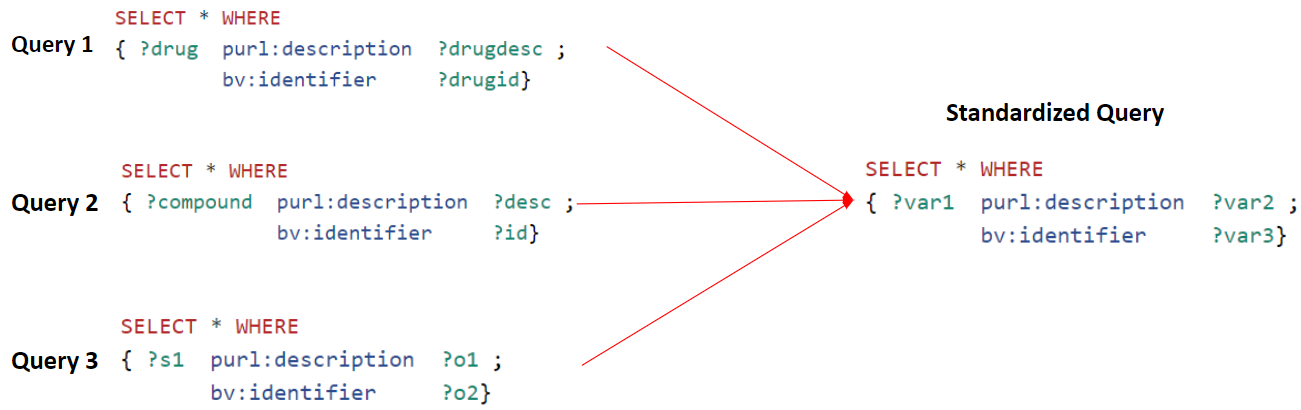
\includegraphics[width=0.8\textwidth]{image17.png} 
    \caption{Variable standardization. ?drug, ?compound, and ?s1, are standardized to ?var1.}
    \label{fig:l2}
\end{figure}
\subsection{Extracting Used Schema Elements }\DIFaddbegin \label{sec:used}
\DIFaddend We write a Python script to extract \DIFdelbegin \DIFdel{"}\DIFdelend \DIFaddbegin \DIFadd{``}\DIFaddend used schema elements\DIFdelbegin \DIFdel{" }\DIFdelend \DIFaddbegin \DIFadd{'' }\DIFaddend from the parse trees of the queries. We first identify \DIFdelbegin \DIFdel{subjects, predicates, and objects elements }\DIFdelend \DIFaddbegin \DIFadd{the subject, predicate, and object IRIs }\DIFaddend within each query\DIFdelbegin \DIFdel{’}\DIFdelend \DIFaddbegin \DIFadd{'}\DIFaddend s parse tree. Then, we determine the intersection of these \DIFdelbegin \DIFdel{elements }\DIFdelend \DIFaddbegin \DIFadd{IRIs }\DIFaddend with the total schema elements that were retrieved earlier.

\DIFaddbegin \paragraph{\textbf{\DIFadd{What we mean by ``used''.}}} \DIFadd{Throughout, a schema element is counted as }\emph{\DIFadd{used}} \DIFadd{if it is }\emph{\DIFadd{explicitly referenced}}\DIFadd{, i.e., its IRI is written in the query text. We deliberately adopt this explicit-reference notion rather than a closure- or answer-based one. As illustrated by the horse example in Section~\ref{s3}.2, a query containing }\texttt{\DIFadd{wdt:P31/wdt:P279* wd:Q726}} \DIFadd{explicitly references only }\texttt{\DIFadd{P31}}\DIFadd{, }\texttt{\DIFadd{P279}}\DIFadd{, and }\texttt{\DIFadd{Q726}}\DIFadd{; the subclasses of horse that the property path traverses at evaluation time (e.g.\ }\emph{\DIFadd{racehorse}}\DIFadd{) contribute to the }\emph{\DIFadd{answers}} \DIFadd{but are not named in the query, and a similar effect arises with property hierarchies. Explicit reference is the appropriate notion for this paper's motivations: documentation, schema and interface design, autocomplete, and deprecation decisions all act on the elements that users and tools actually }\emph{\DIFadd{write}}\DIFadd{, not on the transitive closure a query happens to traverse. We quantified how often the two notions could diverge by measuring property-path usage. Property paths of any kind appear in only about 1\% of valid Bio2RDF organic queries (98 of 8,140), but in 21.1\% of Wikidata organic queries in 2017 (18,705 of 88,491) and 13.7\% in 2018 (25,351 of 185,443); restricting to the transitively-traversing }\texttt{\DIFadd{*}}\DIFadd{/}\texttt{\DIFadd{+}} \DIFadd{operators --- the ones that could actually pull in additional schema elements --- the 2017 figure is 16.6\% (14,696 of 88,491). The explicit-reference and closure-based notions therefore coincide for nearly all Bio2RDF queries, whereas for Wikidata a non-trivial fraction of queries traverse the subclass hierarchy that a closure-based notion would additionally credit.
}

\DIFadd{We can bound this divergence directly. In the 2017 organic queries, the subclass-traversing paths (}\texttt{\DIFadd{wdt:P279*}}\DIFadd{, }\texttt{\DIFadd{wdt:P31/wdt:P279*}}\DIFadd{) are anchored at 1,276 distinct classes; the transitive subclass closure of those anchors, computed from the 2017 dump's 2.08M }\texttt{\DIFadd{P279}} \DIFadd{edges, spans 64,843 of the KG's $\sim$103,000 classes, of which 62,410 are not named explicitly. A closure/answer-based ``effective usage'' notion would therefore credit up to those 62,410 additional types, raising organic coverage from $\sim$4\% to $\sim$62\% --- a $+60$ percentage-point swing. Crucially, this bound is dominated by a handful of queries anchored at near-root classes: }\texttt{\DIFadd{wdt:P279*}} \DIFadd{from }\emph{\DIFadd{entity}} \DIFadd{(}\texttt{\DIFadd{Q35120}}\DIFadd{) alone, used in just 13 queries, has a closure of 64,356 classes, and }\emph{\DIFadd{concept}} \DIFadd{(}\texttt{\DIFadd{Q151885}}\DIFadd{) 49,828, whereas typical anchors are small (}\emph{\DIFadd{city}} \DIFadd{96, }\emph{\DIFadd{film}} \DIFadd{94, }\emph{\DIFadd{organization}} \DIFadd{3,538). A closure-based metric is thus not merely harder to compute but ill-behaved on an item-based KG: a single query rooted at }\emph{\DIFadd{entity}} \DIFadd{would mark most of the ontology as ``used,'' conflating }\emph{\DIFadd{queried}} \DIFadd{with }\emph{\DIFadd{reachable in principle}}\DIFadd{. This is positive evidence for the explicit-reference choice; a principled, partially-credited closure measure remains future work (Section~\ref{s5}).
}

\DIFaddend \subsection{Calculating Schema Coverage}
Equation \ref{eq:1} was used to calculate the SPARQL Schema Coverage (SC). This metric quantifies the proportion of the KG schema that is used by user queries. SC is the ratio of Used Schema Elements (USE) to Total Schema Elements (TSE) in the KG, multiplied by 100 to express the result as a percentage. The TSE represents the count of all distinct types and predicates in the KG, while the USE denotes the count of those classes and predicates found in user SPARQL query logs. We obtained the values for USE and TSE from the results of the previously described steps. \DIFaddbegin \DIFadd{Coverage is always reported against a }\emph{\DIFadd{clearly delimited reference set}}\DIFadd{: the numerator and denominator are derived from the same set of subgraphs (Section~\ref{s4}.1), and we report types and predicates separately (Table~\ref{tab:4}) rather than only their sum. Because the type sets of Bio2RDF and Wikidata are constructed differently (OWL-style vocabulary IRIs vs.\ the data-driven }\texttt{\DIFadd{wdt:P31}}\DIFadd{/}\texttt{\DIFadd{wdt:P279}} \DIFadd{operationalization of Section~\ref{s3}.2) and differ in scale by roughly two orders of magnitude, coverage percentages are meaningful }\emph{\DIFadd{within}} \DIFadd{a KG (across query types and time) but should not be read as a direct cross-KG comparison.
}\DIFaddend \begin{equation}
SC (\%) = \left( \frac{USE}{TSE} \right) \times 100
\label{eq:1}
\end{equation}

\subsection{Identifying Content Usage Patterns}\label{sec:s6}
Up to this point, we have introduced a method for calculating SPARQL schema coverage, which measures the proportion of schema elements in a KG that are queried. However, this metric alone does not reveal how frequently individual schema elements are used or whether their usage is consistent over time. Step six involves analyzing the frequency distribution of the schema elements, identifying frequently used elements, and detecting commonalities in robotic and organic logs, or across different time periods. Additionally, we apply statistical tests, including the Wilcoxon signed-rank test and Spearman's rank correlation coefficient, to assess the consistency and changes in the frequency and ranking of schema element usage over time. The following sections provide a detailed explanation of these methods, with the findings presented in the Results section.

\subsubsection{Frequency Distribution of Schema Elements}\label{sec:s61}
To analyze and compare the frequency distributions of schema elements across multiple datasets, we normalize the usage count of each element to account for varying time intervals. We calculate the monthly frequency of each element by dividing its total count by the log collection period \DIFaddbegin \DIFadd{expressed in months }\DIFaddend (Equation \ref{eq:2}). \DIFaddbegin \DIFadd{Here one month is a fixed 30-day period, so the normalized count has units of }\emph{\DIFadd{uses per 30-day month}} \DIFadd{(it is not dimensionless). }\DIFaddend To reduce skewness and enhance interpretability, we apply a logarithmic transformation (\DIFdelbegin \DIFdel{log10}\DIFdelend \DIFaddbegin \DIFadd{$\log_{10}$}\DIFaddend ) to these normalized counts. Finally, we visualize the normalized frequency distribution of schema elements across different datasets to facilitate comparison.

\begin{equation}
\text{Normalized count} = \frac{\text{Total count}}{\text{log collection period}}
\label{eq:2}
\end{equation}

\DIFdelbegin \DIFdel{We perform the Shapiro-Wilk test (SW) (Equation \ref{eq:shapiro}) to checkthe normality of the differences in the frequencies of common schema elements }\DIFdelend \DIFaddbegin \DIFadd{Before comparing the two intervals statistically, we must decide whether a parametric (normality-assuming) test is appropriate. The Shapiro--Wilk test (Equation~\ref{eq:shapiro}) assesses whether a sample plausibly comes from a normal distribution; we use it purely as a precondition check. We apply it to the per-element }\emph{\DIFadd{change}} \DIFadd{in normalized usage frequency }\DIFaddend between the two intervals \DIFdelbegin \DIFdel{of the query logs}\DIFdelend \DIFaddbegin \DIFadd{(defined below). We emphasize that normality here is a property of these numeric differences (real numbers, naturally ordered), not of any ordering over the schema elements themselves}\DIFaddend .

\begin{equation}
SW = \frac{\left( \sum_{i=1}^n a_i x_i \right)^2}{\sum_{i=1}^n (x_i - \bar{x})^2}
\label{eq:shapiro}
\end{equation}

where \DIFaddbegin \DIFadd{the }\DIFaddend \( x_i \) are the ordered sample values, \DIFdelbegin \DIFdel{in our case, the differences in normalized counts between the two intervals: }\textit{\DIFdel{\( x_i = \text{diff} = \text{Normalized\_schema\_count\_Interval\_2} - \text{Normalized\_schema\_count\_Interval\_1} \)}}%DIFAUXCMD
\DIFdel{, }\DIFdelend \( \bar{x} \) is the sample mean, and \DIFaddbegin \DIFadd{the }\DIFaddend \( a_i \) are \DIFdelbegin \DIFdel{constants based on the sample size.
}\DIFdelend \DIFaddbegin \DIFadd{the Shapiro--Wilk coefficients, i.e., tabulated constants derived from the expected values and covariances of the order statistics of a standard-normal sample of size \( n \). In our case each \( x_i \) is, for one schema element common to both intervals, the change in its normalized monthly usage frequency from the first interval to the second (interval-2 value minus interval-1 value).
}\DIFaddend 


The \DIFdelbegin \DIFdel{results of this test showed a p-value of zero }\DIFdelend \DIFaddbegin \DIFadd{test returned $p \approx 0$ }\DIFaddend for both the Wikidata and Bio2RDF \DIFdelbegin \DIFdel{intervals meaning that the differences }\DIFdelend \DIFaddbegin \DIFadd{interval pairs, so the per-element changes }\DIFaddend are not normally distributed. \DIFdelbegin \DIFdel{Therefore, we performed the }\DIFdelend \DIFaddbegin \DIFadd{We therefore use the non-parametric }\DIFaddend Wilcoxon signed-rank test (\DIFdelbegin \DIFdel{W) (Equation\ref{eq:wilcoxon}) to measure the consistency in the usage frequency of common schema elements }\DIFdelend \DIFaddbegin \DIFadd{Equation~\ref{eq:wilcoxon}), which compares the same schema element measured in two intervals (a paired design) without assuming normality, to test whether usage frequencies shifted significantly }\DIFaddend between the two intervals\DIFdelbegin \DIFdel{of the query logs}\DIFdelend .

\begin{equation}
W = \sum_{i=1}^n \text{sign}(d_i) R_i
\label{eq:wilcoxon}
\end{equation}

where \(d_i\) is the difference between the usage frequency of schema elements (in two intervals), \( \text{sign}(d_i) \) is the sign of \(d_i\), and \(R_i\) is the rank of the absolute differences.


\paragraph{\textbf{Changes in Used Schema Element Ranking.}}
\DIFdelbegin \DIFdel{To measure the consistency in the ranking of common schema elements between two intervals of query logs, we calculate }\DIFdelend \DIFaddbegin \DIFadd{The Wilcoxon test addresses changes in usage }\emph{\DIFadd{magnitude}}\DIFadd{; we separately ask whether the relative }\emph{\DIFadd{popularity ranking}} \DIFadd{of schema elements is stable over time. We rank elements by their normalized usage frequency within each interval (rank 1 = most frequently used) and compute }\DIFaddend Spearman's rank correlation coefficient (\( \rho \)) (Equation\DIFdelbegin \DIFdel{\ref{eq:4}). This metric evaluates the degree of correlation in the ranksof schema elements across these two time points, capturing general trends in rank order consistency. \(d_i\) }\DIFdelend \DIFaddbegin \DIFadd{~\ref{eq:4}) between the two rankings. Spearman's \( \rho \) is the Pearson correlation of the ranks; it summarizes in a single number in \([-1,1]\) whether elements that were popular in one interval remained popular in the other, and it is distribution-free, which suits our non-normal data. Here \( d_i \) }\DIFaddend is the difference between the ranks of \DIFdelbegin \DIFdel{corresponding schema elements, and n }\DIFdelend \DIFaddbegin \DIFadd{schema element \( i \) in the two intervals, and \( n \) }\DIFaddend is the number of \DIFdelbegin \DIFdel{observations \mbox{%DIFAUXCMD
\cite{spearman1961proof}}\hskip0pt%DIFAUXCMD
. }\DIFdelend \DIFaddbegin \DIFadd{common schema elements \mbox{%DIFAUXCMD
\cite{spearman1961proof}}\hskip0pt%DIFAUXCMD
. We use Spearman's \( \rho \) as a compact measure of temporal }\emph{\DIFadd{stability}}\DIFadd{, complementing the Wilcoxon test.
}\DIFaddend \begin{equation}
\rho = 1 - \frac{6 \sum d_i^2}{n(n^2 - 1)}
\label{eq:4}
\end{equation}

% To measure the proportion of schema element pairs that maintain their relative rank ordering between the two intervals, we calculate the concordance index (equation~\ref{eq:5}), where concordant pairs are defined as a pair of schema elements \( (i, j) \) that their relative ranks are the same in both intervals.

% \begin{equation}
%     \text{C-index} = \frac{\text{Number of concordant pairs}}{\text{Total number of pairs}}
%     \label{eq:5}
% \end{equation}


\subsubsection{Frequent Schema Elements} \label{sec:s62}
We analyze the most frequently queried schema types from robotic and organic logs of Wikidata and Bio2RDF to identify common elements that persist across different time intervals and log types. \DIFaddbegin \DIFadd{This focus on the most frequent elements is similar in spirit to the predicate-frequency analysis of Bonifati et al.\ \mbox{%DIFAUXCMD
\cite{bonifati2019navigating}}\hskip0pt%DIFAUXCMD
, to which we add the temporal and organic/robotic dimensions. }\DIFaddend While our ranking analysis of all schema elements reveals broad usage dynamics and temporal shifts, we're particularly interested in determining whether a subset of frequently accessed elements remains consistently popular over time, indicating their significance as "core" elements of the KG. The presence of a stable core across the datasets would suggest that these elements are central to the KG’s utility, regardless of the query time or type. \DIFdelbegin \DIFdel{To investigate this}\DIFdelend \DIFaddbegin \DIFadd{This frequent-element analysis is computed over schema }\emph{\DIFadd{types}} \DIFadd{(classes); predicates, whose frequency distribution is dominated by a few generic relations, are analyzed separately. To investigate the stable core}\DIFaddend , we first examine the top 10 schema \DIFdelbegin \DIFdel{elements }\DIFdelend \DIFaddbegin \DIFadd{types }\DIFaddend in each dataset, as they represent the most frequently queried components, as well as the top 50 \DIFdelbegin \DIFdel{elements}\DIFdelend \DIFaddbegin \DIFadd{types}\DIFaddend . The top 50 threshold strikes a balance by providing a more comprehensive view of usage patterns compared to the top 10 while still avoiding the inclusion of many low-frequency \DIFdelbegin \DIFdel{elements}\DIFdelend \DIFaddbegin \DIFadd{types}\DIFaddend . For example, in Wikidata 2017, the frequency for \DIFdelbegin \DIFdel{elements }\DIFdelend \DIFaddbegin \DIFadd{types }\DIFaddend ranked 51 to 3560 ranges from 149 to 1, whereas the top 50 \DIFdelbegin \DIFdel{elements }\DIFdelend \DIFaddbegin \DIFadd{types }\DIFaddend have frequencies between 6,962 and 150. To analyze schema usage patterns, we visualize frequently queried schema elements and identify common elements across datasets, log types, and time intervals. This approach aims to determine whether there is a set of core schema elements that drives query activity in these KGs.


\paragraph{\textbf{Pairwise Schema Type Usage of Bio2RDF.}}
Bio2RDF consists of 26 interconnected subgraphs, each representing a distinct dataset with its own vocabulary. These subgraphs are linked through various predicates. For example, the \url{ctd_vocabulary:Gene-Disease-Association} type from the "ctd" subgraph and the \url{ncbigene_vocabulary:Resource} from the "ncbigene" subgraph are linked by the predicate \url{ctd_vocabulary:gene}, establishing a relationship between the two elements. A typical triple pattern representing the connection between two distinct subgraphs is: \sloppy \texttt{?schema\_Type\_from\_first\_subgraph ?predicate ?schema\_Type\_from\_second\_subgraph}. This relationship is referred to as a "pairwise schema type pattern."

Bio2RDF’s subgraph organization enables an analysis of how frequently queries capture relationships between schema types from different subgraphs. However, since Wikidata does not have an explicit subgraph structure, this type of analysis is not applicable to its dataset. To investigate this type of usage, we conduct an experiment comparing Bio2RDF query logs from 2013 and 2019 to determine how often datasets (or subgraphs) were integrated in queries to retrieve more complex information. The approach consists of two main steps:

\textbf{Identifying total pairwise schema type patterns.} We extract all possible pairwise schema type patterns from the Bio2RDF schema, covering 17 subgraphs in log\_2013 and 26 subgraphs in log\_2019.


\textbf{Identifying pairwise schema type pattern occurrences in logs.} We analyze the triple patterns within queries to identify occurrences of these pairwise schema type patterns. For each dataset, we construct a matrix where both rows and columns represent schema type subgraphs. Each cell in the matrix corresponds to a specific pair of subgraphs, and its value indicates the frequency of the pattern in the queries.
By conducting this analysis, we aim to discover how often queries integrate information across Bio2RDF subgraphs and how this usage has evolved over time.

\section{Results}\label{s4}
In this section, we describe the results of the various steps in the method, including the retrieval of datasets, the pre-processing of SPARQL queries, the extraction of all schema elements, the extraction of the schema elements used, the calculation of the SPARQL schema coverage, and the analysis of usage patterns.

\subsection{Dataset Retrieval }
Table \ref{tab:1} provides an overview of the datasets retrieved for analysis, including the logs from Bio2RDF and Wikidata KGs for multiple periods and query types. \DIFdelbegin \DIFdel{The "}\DIFdelend \DIFaddbegin \DIFadd{We use a single naming convention of the form }\emph{\DIFadd{KG-agenttype-period}[\DIFadd{-interval}] \DIFadd{(KG version)}}\DIFadd{; for example, }\emph{\DIFadd{Bio2RDF-all-2013}} \DIFadd{is the full 2013 }\DIFaddend Bio2RDF \DIFdelbegin \DIFdel{log2013" }\DIFdelend \DIFaddbegin \DIFadd{log and }\emph{\DIFadd{Wikidata-organic-2017-int1}} \DIFadd{is interval~1 of the 2017 Wikidata organic log. The }\emph{\DIFadd{Bio2RDF-all-2013}} \DIFadd{log }\DIFaddend originates from LSQ and spans 16.79 months, from May 2013 to September 2014, containing 31,950,877 queries. This \DIFaddbegin \DIFadd{LSQ-derived }\DIFaddend dataset lacks user-agent information and only includes the \DIFdelbegin \DIFdel{lsqv:hostHash }\DIFdelend \DIFaddbegin \texttt{\DIFadd{lsqv:hostHash}} \DIFaddend property, an anonymized hash of the host or IP address issuing each query\DIFaddbegin \DIFadd{; the LSQ release therefore cannot itself be split into organic and robotic. To recover that split for the 2013 era we additionally obtained the }\emph{\DIFadd{raw}} \DIFadd{Bio2RDF server access log (the upstream source from which LSQ was built, spanning May 2013--September 2015), which retains user agents; we use it to characterize 2013-era organic vs.\ robotic traffic in Section~\ref{sec:bio2013}}\DIFaddend . \DIFdelbegin \DIFdel{As a result, it was not possible to decide whether queries are organic or robotic . }\DIFdelend The second dataset, \DIFdelbegin \DIFdel{"Bio2RDF log2019" }\DIFdelend \DIFaddbegin \emph{\DIFadd{Bio2RDF-all-2019}}\DIFadd{, }\DIFaddend covers a longer period of 29.93 months, from January 2019 to July 2021. It \DIFdelbegin \DIFdel{contains a total of }\DIFdelend \DIFaddbegin \DIFadd{comprises }\DIFaddend 3,880,960 \DIFdelbegin \DIFdel{queries, of which }\DIFdelend \DIFaddbegin \DIFadd{log entries. Of these, }\DIFaddend 3,212 are \DIFdelbegin \DIFdel{server logs, and do not contain SPARQL queries. The resulting dataset includes }\DIFdelend \DIFaddbegin \DIFadd{server-side log lines that contain no SPARQL query, leaving }\DIFaddend 3,877,748 SPARQL queries. This dataset \DIFdelbegin \DIFdel{provides }\DIFdelend \DIFaddbegin \DIFadd{retains }\DIFaddend user-agent information\DIFdelbegin \DIFdel{to differentiate between }\DIFdelend \DIFaddbegin \DIFadd{, allowing us to separate }\DIFaddend robotic (3,816,776\DIFdelbegin \DIFdel{queries}\DIFdelend ) and organic (56,736\DIFdelbegin \DIFdel{queries) traffic. However, }\DIFdelend \DIFaddbegin \DIFadd{) queries; a further }\DIFaddend 7,427 queries lack user-agent information \DIFaddbegin \DIFadd{and are excluded from the split}\DIFaddend .

Wikidata logs contain both organic and robotic queries. The \DIFdelbegin \DIFdel{"Wikidata organic log2017" }\DIFdelend \DIFaddbegin \emph{\DIFadd{Wikidata-organic-2017-full}} \DIFadd{log }\DIFaddend spans 9.43 months, from June 2017 to March 2018, and consists of 3,298,254 organic queries. \DIFdelbegin \DIFdel{In contrast, the "Wikidata organic log2017" and the "Wikidata organic log2018" }\DIFdelend \DIFaddbegin \DIFadd{The shorter, interval-based slices used for the temporal comparison }\DIFaddend were collected over only 0.88 months \DIFdelbegin \DIFdel{, comprising }\DIFdelend \DIFaddbegin \DIFadd{each: }\emph{\DIFadd{Wikidata-organic-2017-int1}} \DIFadd{and }\emph{\DIFadd{Wikidata-organic-2018-int7}} \DIFadd{comprise }\DIFaddend 192,331 and 872,556 organic queries, respectively\DIFdelbegin \DIFdel{. Similarly, the "Wikidata robotic log2017" and the "Wikidata robotic log2018" were collected over 0.88 months, containing }\DIFdelend \DIFaddbegin \DIFadd{, while }\emph{\DIFadd{Wikidata-robotic-2017-int1}} \DIFadd{and }\emph{\DIFadd{Wikidata-robotic-2018-int7}} \DIFadd{contain }\DIFaddend 59,355,579 and 81,339,186 robotic queries, respectively.

\begin{table}[h!]
\centering
\caption{Results of \DIFaddbeginFL \DIFaddFL{the }\DIFaddendFL data retrieval step\DIFaddbeginFL \DIFaddFL{. Datasets follow the naming convention }\emph{\DIFaddFL{KG-agenttype-period}[\DIFaddFL{-interval}]}\DIFaddFL{; ``All'' denotes the union of organic and robotic queries (not a superset of any single row).}\DIFaddendFL }
\label{tab:1}
\begin{tabular}{l|r|l|r} 
\hline
\textbf{Dataset} & \#\textbf{Queries} & \textbf{log collection period} & \textbf{Duration (months)} \\ \hline
Bio2RDF All log2013 & 31,950,877 & 2013-05-05 to 2014-09-28 & 16.79 \\ 
Bio2RDF All log2019 & 3,880,960  & 2019-01-07 to 2021-07-06 & 29.93 \\ 
Bio2RDF robotic log2019 & 3,816,776  & 2019-01-07 to 2021-07-06 & 29.93 \\ 
Bio2RDF organic log2019 & 56,736 & 2019-01-07 to 2021-07-06 & 29.93 \\ 
Wikidata All organic log2017 & 3,298,254 & 2017-06-11 to 2018-03-25 & 9.43 \\ 
Wikidata robotic log2017 & 59,355,579 & 2017-06-12 to 2017-07-09 & 0.88 \\ 
Wikidata robotic log2018 & 81,339,186 & 2018-02-26 to 2018-03-25 & 0.88 \\ 
 Wikidata organic log2017&
192,331&
2017-06-12 to 2017-07-09&
0.88\\
Wikidata organic log2018&
872,556&
 2018-02-26 to 2018-03-25&
0.88\\
\hline
\end{tabular}
\end{table}

During our analysis in 2024, the Bio2RDF SPARQL endpoint contained 26 subgraphs/datasets. However, the Bio2RDF log2013 and Bio2RDF log2019 datasets do not contain query logs corresponding to all 26 subgraphs. Figures \ref{fig:l3} and \ref{fig:l4} provide details through Venn diagrams: Figure \ref{fig:l3} illustrates the overlap between the Bio2RDF log2013 datasets and the KG subgraphs, while Figure \ref{fig:l4} represents the Bio2RDF log2019 datasets compared to the KG subgraphs in the 2024 endpoint. This comparison highlights the importance of using a consistent reference set when calculating schema coverage (Equation \ref{eq:1}). That is, the numerator and denominator (i.e., used and total schema elements) should be derived from the same set of datasets, ensuring alignment between KG subgraphs and log datasets.

The Venn diagram in Figure \ref{fig:l3} compares the datasets included in Bio2RDF log2013 with the subgraphs in Bio2RDF KG2024. The left oval represents datasets unique to Bio2RDF log2013. The overlapping section in the center lists 17 datasets common to both Bio2RDF log2013 and Bio2RDF KG2024. The right oval represents datasets unique to Bio2RDF KG2024.


The Venn diagram in Figure \ref{fig:l4} compares the datasets included in Bio2RDF log2019 with the subgraphs in Bio2RDF KG2024. The left oval represents datasets unique to Bio2RDF log2019. The overlapping section in the center lists 22 datasets common to both Bio2RDF log2019 and Bio2RDF KG2024. The right oval represents datasets unique to Bio2RDF KG2024. 

The  dataset "Bio2RDF" in log2019 refers to the logs of a general endpoint for all subgraphs and may include queries to the HP, ECO, APO, and GO subgraphs. This is because, historically, Bio2RDF maintained a distinct SPARQL endpoint for each subgraph. Later, a single general endpoint was introduced to host all subgraphs for querying.


\begin{figure}
    \centering
    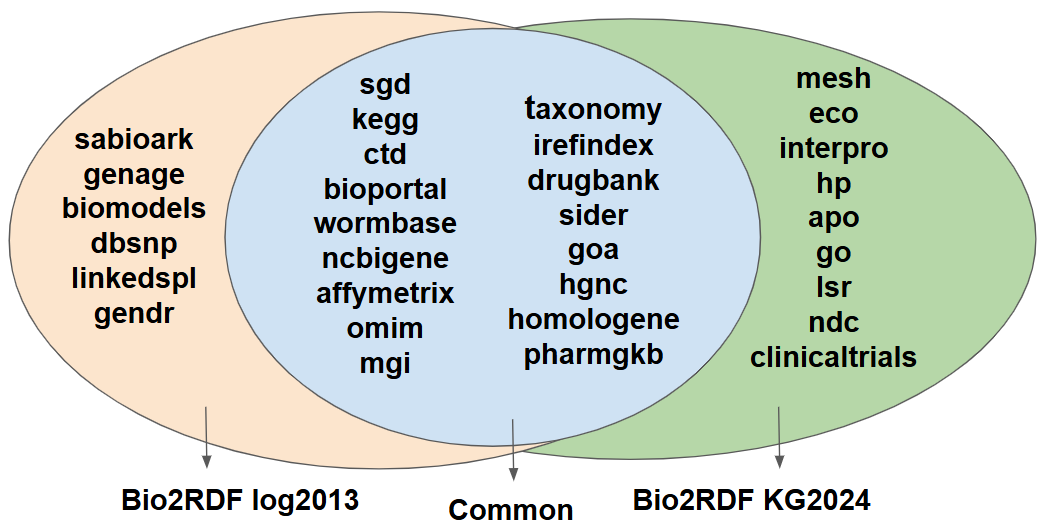
\includegraphics[width=0.53\textwidth]{image9.png} 
    \caption{Venn diagram illustrating the overlap  between the Bio2RDF log2013 datasets and the Bio2RDF KG 2024
}
    \label{fig:l3}
\end{figure}

\begin{figure}[htbp]
    \centering
    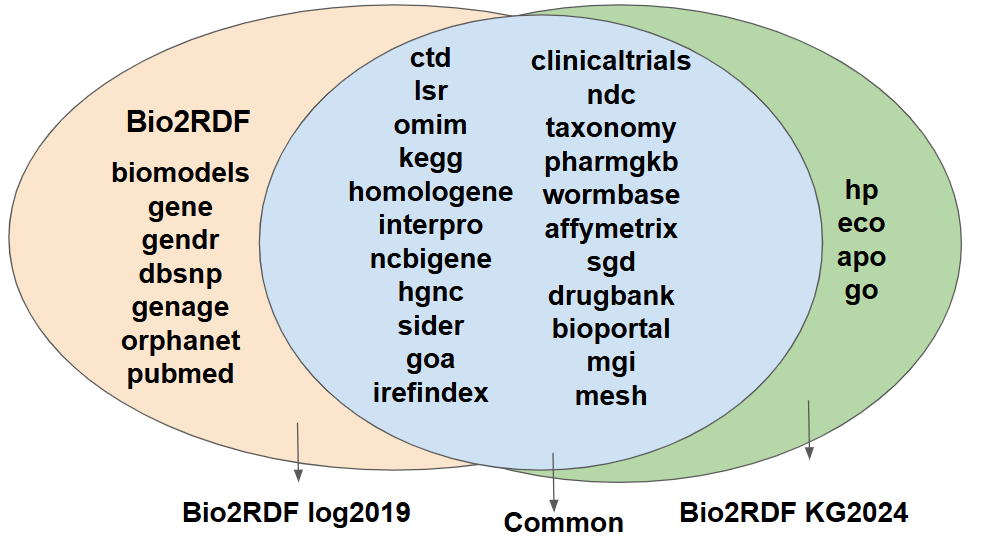
\includegraphics[width=0.55\textwidth]{image8.png} 
    \caption{ Venn diagram illustrating the overlap between the Bio2RDF log2019 datasets and the Bio2RDF KG 2024
}
     \label{fig:l4}
\end{figure}


\subsection{Extracting Total Schema Elements}
Table \ref{tab:3} presents the statistics of total schema elements across different KG versions. Initially, the Bio2RDF schema comprised 166,444 unique types. After excluding types that do not adhere to the template \url{http://Bio2RDF.org/DATASET_vocabulary:SCHEMA_ELEMENT}',' 545 types remain. A further refinement, by excluding elements with the template \url{'http://Bio2RDF.org/DATASET_vocabulary:Resource,'} reduces the count to 350 types and 195 predicates, distributed across 26 subgraphs within the Bio2RDF KG on the current endpoint (2024). Out of these 26 subgraphs, only 17 have corresponding query logs available in the Bio2RDF log2013 dataset, as depicted in Figure \ref{fig:l3}. These 17 subgraphs contain 270 types and 129 predicates, in total 399 schema elements.

As represented in Table \ref{tab:3}, the Wikidata KG version 2017 contains 103,380 types, whereas the Wikidata KG version 2018 contains 97,470 types, reflecting a reduction in the number of schema types. These results illustrate the variability in schema complexity with Wikidata exhibiting a larger and more diverse set of schema elements compared to Bio2RDF.
\begin{table}[ht]
\centering
\caption{Total schema elements Statistics per KG version}
\label{tab:3}
\resizebox{\textwidth}{!}{
\begin{tabular}{l|r|r|r|r}
\hline
Source & Bio2RDF KG2024 (17 subgraphs) & Bio2RDF KG2024 (26 subgraphs) & Wikidata KG2017 & Wikidata KG2018 \\
\hline
Total number of distinct Elements & 399 & 545 & 104,314 & 98,462 \\
Number of distinct Types & 270 & 350 & 103,380 & 97,470 \\
Number of distinct Predicates & 129 & 195 & 934 & 992 \\
\hline
\end{tabular}
}
\end{table}


\subsection{Preprocessing SPARQL Queries}
Table \ref{tab:2} summarizes the number of queries (\#Queries), unique queries (\#Unique), \DIFdelbegin \DIFdel{unique syntactically correct }\DIFdelend \DIFaddbegin \DIFadd{queries with incorrect syntax (\#Failed to parse), and unique syntactically valid }\DIFaddend queries (\#Valid) \DIFaddbegin \DIFadd{across all datasets. We emphasize the Bio2RDF~2019 rows: with the corrected preprocessing, the number of valid queries is far higher than under the earlier pipeline (e.g., for robotic~2019}\DIFaddend , \DIFdelbegin \DIFdel{standardized valid queries (\#Normalized), and queries with incorrect syntax (\#Failed to parse)across all datasets}\DIFdelend \DIFaddbegin \DIFadd{1}{\DIFadd{,}}\DIFadd{034}{\DIFadd{,}}\DIFadd{831 vs.\ 627}{\DIFadd{,}}\DIFadd{314), because previously the appended HTTP parameters had caused a large share of well-formed queries to be discarded. The LSQ-sourced Bio2RDF~2013 and the Dresden-sourced Wikidata logs were cleanly extracted and reproduce closely (validity rates of 99.8\% and $>$99.9\% respectively), confirming that the parsing defect was specific to the raw Bio2RDF~2019 server logs and does not affect the schema-coverage results, which are computed over the same valid queries}\DIFaddend .

% We reviewed the 416,896 queries in the Bio2RDF log 2019 that failed to parse. Approximately 300,000 of the 416,896 failures were simple templates with varying LIMIT and OFFSET values, as shown in Listing \ref{lst:third_list} 6 with a syntactic error. More than 1,819 of these queries were not SPARQL queries at all; rather, they were plain text, mostly in English. For example, one such message reads: "I love your blog... very nice colors \& theme. Did you make ...". Interestingly, the execution agent for these queries is Mozilla, rather than Java, Python, or any web crawler. Nine queries contained only the string "/sparql." 
% \begin{center}
% \begin{minipage}{0.76\textwidth} % Adjust width here (e.g., 0.9 for 90% of text width)
% \begin{lstlisting}[caption={The templated SPARQL query against the LSQ SPARQL endpoint to retrieve SPARQL queries for selected datasets.}]
% -- Query 1

%     SELECT ?r (COUNT(*) AS ?count) WHERE { ?r ?s ?o } 
%     OFFSET 177863205 LIMIT 1000 
%     GROUP BY ?rOFFSET 0 LIMIT 10000

%  -- Query 2

%     SELECT ?r (COUNT(*) AS ?count) WHERE { ?r ?s ?o } 
%     OFFSET 62950773 LIMIT 1000 
%     GROUP BY ?rOFFSET 0 LIMIT 10000

% -- Query 3

%     SELECT ?r (COUNT(*) AS ?count) WHERE { ?r ?s ?o } 
%     OFFSET 85005378 LIMIT 1000 
%     GROUP BY ?rOFFSET 0 LIMIT 10000

% \end{lstlisting}
% \label{lst:third_list}
% \end{minipage}
% \end{center}

\begin{table}[ht]
\centering
\caption{Results of \DIFdelbeginFL \DIFdelFL{Parsing }\DIFdelendFL \DIFaddbeginFL \DIFaddFL{parsing }\DIFaddendFL and \DIFdelbeginFL \DIFdelFL{Variable Standardization in Query Logs}\DIFdelendFL \DIFaddbeginFL \DIFaddFL{validating the query logs, regenerated with the
corrected preprocessing (full HTTP query-string parameter stripping applied before
deduplication, base-IRI resolution of relative IRIs). \#Failed-to-parse $=$ \#Unique
$-$ \#Valid. \#Valid is computed with a SPARQL~1.1 parser (sparqljs). The Bio2RDF~2019
rows change substantially relative to earlier processing because appended HTTP
parameters (notably }\texttt{\DIFaddFL{\&callback}}\DIFaddFL{) had previously caused many valid queries to be
rejected; the LSQ-sourced (Bio2RDF~2013) and Dresden-sourced (Wikidata) logs were
already cleanly extracted and reproduce. The Bio2RDF~2013 figures use the executed-query
set (queries with a recorded remote execution).}\DIFaddendFL }
\label{tab:2}
\DIFdelbeginFL %DIFDELCMD < \begin{tabular}{l|r|r|r|r|r}
%DIFDELCMD < %%%
\DIFdelendFL \begin{tabular}{l|r|r|r|r}
\hline
Dataset & \#SPARQL Queries & \#Unique & \#Failed to parse & \#Valid \DIFdelbeginFL %DIFDELCMD < & %%%
\DIFdelFL{\#Normalized }\DIFdelendFL \\
\hline
Bio2RDF All log2013 & 31,950,877 & 1,519,\DIFdelbeginFL \DIFdelFL{793 }\DIFdelendFL \DIFaddbeginFL \DIFaddFL{681 }\DIFaddendFL & \DIFdelbeginFL \DIFdelFL{5,249 }\DIFdelendFL \DIFaddbeginFL \DIFaddFL{2,521 }\DIFaddendFL & 1,\DIFdelbeginFL \DIFdelFL{514,544 }%DIFDELCMD < & %%%
\DIFdelFL{1,486,540 }\DIFdelendFL \DIFaddbeginFL \DIFaddFL{517,160 }\DIFaddendFL \\
Bio2RDF All log2019 & 3,\DIFdelbeginFL \DIFdelFL{877,748 }\DIFdelendFL \DIFaddbeginFL \DIFaddFL{880,939 }\DIFaddendFL & 1,\DIFdelbeginFL \DIFdelFL{048,592 }\DIFdelendFL \DIFaddbeginFL \DIFaddFL{050,616 }\DIFaddendFL & \DIFdelbeginFL \DIFdelFL{7,444 }\DIFdelendFL \DIFaddbeginFL \DIFaddFL{9,950 }\DIFaddendFL & \DIFdelbeginFL \DIFdelFL{634,783 }%DIFDELCMD < & %%%
\DIFdelFL{632,622 }\DIFdelendFL \DIFaddbeginFL \DIFaddFL{1,040,666 }\DIFaddendFL \\
Bio2RDF robotic log2019 & 3,\DIFdelbeginFL \DIFdelFL{816,776 }\DIFdelendFL \DIFaddbeginFL \DIFaddFL{824,203 }\DIFaddendFL & 1,\DIFdelbeginFL \DIFdelFL{039,411 }\DIFdelendFL \DIFaddbeginFL \DIFaddFL{040,356 }\DIFaddendFL & 5,\DIFdelbeginFL \DIFdelFL{927 }\DIFdelendFL \DIFaddbeginFL \DIFaddFL{525 }\DIFaddendFL & \DIFdelbeginFL \DIFdelFL{627,314 }%DIFDELCMD < & %%%
\DIFdelFL{625,594 }\DIFdelendFL \DIFaddbeginFL \DIFaddFL{1,034,831 }\DIFaddendFL \\
Bio2RDF organic log2019 & \DIFdelbeginFL \DIFdelFL{53,524 }\DIFdelendFL \DIFaddbeginFL \DIFaddFL{56,736 }\DIFaddendFL & \DIFdelbeginFL \DIFdelFL{9,612 }\DIFdelendFL \DIFaddbeginFL \DIFaddFL{12,579 }\DIFaddendFL & \DIFdelbeginFL \DIFdelFL{1,517 }\DIFdelendFL \DIFaddbeginFL \DIFaddFL{4,439 }\DIFaddendFL & \DIFdelbeginFL \DIFdelFL{7,357 }%DIFDELCMD < & %%%
\DIFdelFL{7,030 }\DIFdelendFL \DIFaddbeginFL \DIFaddFL{8,140 }\DIFaddendFL \\
Wikidata All organic log2017 & 3,\DIFdelbeginFL \DIFdelFL{298,254 }\DIFdelendFL \DIFaddbeginFL \DIFaddFL{530,948 }\DIFaddendFL & \DIFdelbeginFL \DIFdelFL{844,256 }\DIFdelendFL \DIFaddbeginFL \DIFaddFL{859,290 }\DIFaddendFL & \DIFdelbeginFL \DIFdelFL{125 }\DIFdelendFL \DIFaddbeginFL \DIFaddFL{321 }\DIFaddendFL & \DIFdelbeginFL \DIFdelFL{844,132 }%DIFDELCMD < & %%%
\DIFdelFL{842,812 }\DIFdelendFL \DIFaddbeginFL \DIFaddFL{858,969 }\DIFaddendFL \\
Wikidata robotic log2017 & 59,355,579 & 8,234,\DIFdelbeginFL \DIFdelFL{097 }\DIFdelendFL \DIFaddbeginFL \DIFaddFL{089 }\DIFaddendFL & \DIFdelbeginFL \DIFdelFL{17 }\DIFdelendFL \DIFaddbeginFL \DIFaddFL{20 }\DIFaddendFL & 8,234,\DIFdelbeginFL \DIFdelFL{080 }%DIFDELCMD < & %%%
\DIFdelFL{8,234,041 }\DIFdelendFL \DIFaddbeginFL \DIFaddFL{069 }\DIFaddendFL \\
Wikidata robotic log2018 & 81,339,186 & 18,\DIFdelbeginFL \DIFdelFL{940,103 }\DIFdelendFL \DIFaddbeginFL \DIFaddFL{939,743 }\DIFaddendFL & \DIFdelbeginFL \DIFdelFL{53 }\DIFdelendFL \DIFaddbeginFL \DIFaddFL{86 }\DIFaddendFL & 18,\DIFdelbeginFL \DIFdelFL{940,050 }%DIFDELCMD < & %%%
\DIFdelFL{18,}\DIFdelendFL 939,\DIFdelbeginFL \DIFdelFL{725 }\DIFdelendFL \DIFaddbeginFL \DIFaddFL{657 }\DIFaddendFL \\
Wikidata organic log2017 & 192,\DIFdelbeginFL \DIFdelFL{331}\DIFdelendFL \DIFaddbeginFL \DIFaddFL{330 }\DIFaddendFL & 88,\DIFdelbeginFL \DIFdelFL{516}\DIFdelendFL \DIFaddbeginFL \DIFaddFL{514 }\DIFaddendFL & 23 & 88,\DIFdelbeginFL \DIFdelFL{493 }%DIFDELCMD < & %%%
\DIFdelFL{88,226}\DIFdelendFL \DIFaddbeginFL \DIFaddFL{491 }\DIFaddendFL \\
Wikidata organic log2018 & 872,\DIFdelbeginFL \DIFdelFL{556}\DIFdelendFL \DIFaddbeginFL \DIFaddFL{555 }\DIFaddendFL & 185,\DIFdelbeginFL \DIFdelFL{482}\DIFdelendFL \DIFaddbeginFL \DIFaddFL{478 }\DIFaddendFL & \DIFdelbeginFL \DIFdelFL{44}\DIFdelendFL \DIFaddbeginFL \DIFaddFL{35 }\DIFaddendFL & 185,\DIFdelbeginFL \DIFdelFL{438}%DIFDELCMD < & %%%
\DIFdelFL{185,050}\DIFdelendFL \DIFaddbeginFL \DIFaddFL{443 }\DIFaddendFL \\
\hline
\end{tabular}
\end{table}


\subsection{Extracting Used Schema Elements} 
Table \ref{tab:4} presents the statistics of used schema elements in various datasets, detailing the total number of distinct elements, types, and predicates identified in the queries. From Bio2RDF log2019\_kg2024, 529 distinct elements were extracted, comprising 334 distinct types and 195 distinct predicates. In comparison, Bio2RDF log2013\_kg2024 contains 317 distinct elements, with 227 distinct types and 90 predicates. The robotic queries for Bio2RDF log2019 match the overall log2019\_kg2024 dataset, both reporting 529 distinct elements, 334 classes, and 195 predicates, while the organic queries yield a much smaller subset of 116 elements, 58 types, and 58 predicates.

For Wikidata, log2017\_kg2017 includes 13,394 distinct elements, 12,590 classes and 804 predicates, while log2017\_kg2018 has 13,900 distinct elements, consisting of 13,054 types and 846 predicates. The robotic queries for Wikidata scale significantly larger, with robotic log2017\_kg2017 containing 59,603 elements, 58,680 types, and 923 predicates, and robotic log2018\_kg2018 reporting 59,582 elements, 58,648 types, and 934 predicates. These results illustrate significant variability in schema usage between robotic and organic logs.
\begin{table}[ht]
\centering
\caption{Used \DIFdelbeginFL \DIFdelFL{Schema Element Statistics per }\DIFdelendFL \DIFaddbeginFL \DIFaddFL{schema-element statistics. Each row is based on a }\emph{\DIFaddFL{pair}} \DIFaddFL{of datasets: a query log and the }\DIFaddendFL KG \DIFdelbeginFL \DIFdelFL{Version }\DIFdelendFL \DIFaddbeginFL \DIFaddFL{version it is evaluated against, written }\emph{\DIFaddFL{log}}\DIFaddFL{\_}\emph{\DIFaddFL{kg}} \DIFaddFL{(e.g.\ }\emph{\DIFaddFL{Bio2RDF-all-log2013\_kg2024}} \DIFaddFL{= the 2013 log matched against the 2024 KG). Counts are over unique normalized queries.}\DIFaddendFL }
\label{tab:4}
\begin{tabular}{l|r|r|r}
\hline
Dataset & Total number of distinct Elements & Number of distinct Types & Number of distinct Predicates \\
\hline
Bio2RDF All log2013\_kg2024 & 317 & 227 & 90 \\
Bio2RDF All log2019\_kg2024 & 529 & 334 & 195 \\
Bio2RDF robotic log2019\_kg2024 &  529 & 334 & 195 \\
Bio2RDF organic log2019\_kg2024 &  116 & 58 & 58 \\
Wikidata All organic log2017\_kg2017 & 13,394 & 12,590 & 804 \\
Wikidata All organic log2017\_kg2018 & 13,900 & 13,054 & 846 \\
Wikidata robotic log2017\_kg2017 & 59,603 & 58,680 & 923 \\
Wikidata robotic log2018\_kg2018 & 59,582 & 58,648 & 934 \\
Wikidata organic log2017\_kg2017 & 4,041 & 3,559 & 482 \\
Wikidata organic log2018\_kg2018 & 4,859 & 4,310 & 549 \\
\hline
\end{tabular}
\end{table}

\subsection{Calculating SPARQL Schema Coverage}
Table \ref{tab:5} presents the SPARQL schema coverage of datasets and provides insight into the extent to which schema elements of different KGs are used in SPARQL queries. Bio2RDF All log2019\_kg2024 and Bio2RDF robotic log2019\_kg2024 achieved the highest schema coverage at 97.06\%, indicating that nearly all schema elements were queried at least once. This is followed by Bio2RDF All log2013\_kg2024, which achieved a schema coverage of 79.44\%.  

In contrast, the Bio2RDF Organic log2019\_kg2024 exhibited a much lower schema coverage of 21.28\%. Similarly, the schema coverage for Wikidata robotic queries in log2017\_kg2017 and log2018\_kg2018 was moderate, at 57.13\% and 60.51\%, respectively. However, the schema coverage for Wikidata organic queries in log2017\_kg2017 and log2018\_kg2018 was significantly lower, at 12.84\% and 14.11\%, respectively.

\begin{table}[ht]
\centering
\caption{SPARQL schema coverage\DIFaddbeginFL \DIFaddFL{. Each row pairs a query log with a KG version (}\emph{\DIFaddFL{log}}\DIFaddFL{\_}\emph{\DIFaddFL{kg}}\DIFaddFL{); coverage is $\mathrm{USE}/\mathrm{TSE}\times100$ over the same reference set of subgraphs. As discussed in Sections~\ref{s3}.5 and \ref{sec:rarefaction}, these percentages are comparable within a KG but not directly across the two KGs.}\DIFaddendFL }
\label{tab:5}
\begin{tabular}{l|r}
\hline
Dataset & SC \\
\hline
Bio2RDF All log2013\_kg2024 & 79.44\% \\
Bio2RDF All log2019\_kg2024 & 97.06\% \\
\textbf{Bio2RDF robotic }log2019\_kg2024 & \textbf{97.06}\%\\
Bio2RDF organic log2019\_kg2024 & 21.28\% \\
Wikidata All organic log2017\_kg2017 & 12.84\% \\
Wikidata All organic log2017\_kg2018 & 14.11\% \\
Wikidata robotic log2017\_kg2017 & 57.13\% \\
\textbf{Wikidata robotic} log2018\_kg2018 & \textbf{60.51}\% \\
Wikidata organic log2017\_kg2017 & 3.87\%  \\
Wikidata organic log2018\_kg2018 & 4.93\%  \\
\hline
\end{tabular}
\end{table}



These results highlight a notable difference in schema coverage between robotic and organic queries across Bio2RDF and Wikidata datasets.
\begin{figure}
    \centering
    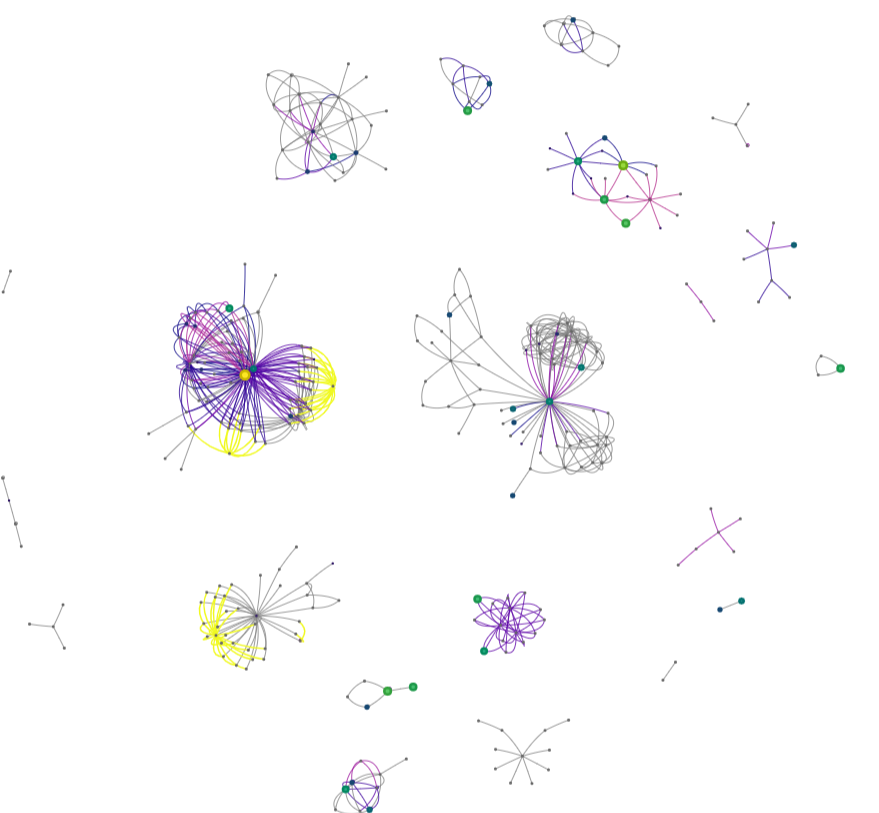
\includegraphics[width=0.6\textwidth]{image21.png} 
    \caption{Visualization of \DIFdelbeginFL \DIFdelFL{the schema element }\DIFdelendFL \DIFaddbeginFL \DIFaddFL{schema-element }\DIFaddendFL usage in \DIFdelbeginFL \DIFdelFL{Bio2RDF organic log2019\_kg2024}\DIFdelendFL \DIFaddbeginFL \emph{\DIFaddFL{Bio2RDF-organic-2019}} \DIFaddFL{(KG2024)}\DIFaddendFL . \DIFaddbeginFL \DIFaddFL{Node size and color both increase with usage frequency (small/dark = rarely used, large/bright = heavily used); edge width increases with predicate usage; schema elements not used in any query are gray. The few large, bright hubs concentrate most of the usage.}\DIFaddendFL }
    \label{fig:l5}
\end{figure}

Figure \ref{fig:l5} illustrates the extent to which \DIFdelbegin \DIFdel{various }\DIFdelend schema elements of \DIFaddbegin \DIFadd{the }\DIFaddend Bio2RDF KG are used in the organic queries of 2019. Nodes represent schema \DIFdelbegin \DIFdel{classes, }\DIFdelend \DIFaddbegin \DIFadd{types }\DIFaddend and edges represent predicates linking \DIFdelbegin \DIFdel{these classes. The size }\DIFdelend \DIFaddbegin \DIFadd{instances of those types. Both the size and the color }\DIFaddend of a node \DIFdelbegin \DIFdel{indicates }\DIFdelend \DIFaddbegin \DIFadd{encode the same quantity, }\DIFaddend its usage frequency\DIFaddbegin \DIFadd{: nodes grow larger and brighter as they are queried more often, while rarely used nodes are small and dark. Edge width likewise grows with predicate usage, and schema elements that appear in no query are shown in gray. The visualization makes the long tail visible directly: a handful of large, bright hubs (drug, gene, and disease types) concentrate the bulk of organic usage, while most of the schema remains gray and unqueried. The interactive version, with exact per-element values, is available online}\footnote{\url{https://marmhm.github.io/Schema-usage-graph/}}\DIFadd{.
}

\subsection{\DIFadd{Size-Controlled Coverage: Is the Organic/Robotic Gap a Sampling Artifact?}}\label{sec:rarefaction}
\DIFadd{The coverage values in Table~\ref{tab:5} could be misleading, because organic and robotic logs differ enormously in size (Table~\ref{tab:2}), and larger samples mechanically touch more vocabulary. To separate a genuine behavioral difference from this sampling effect, we treat each occurrence of a schema element in a log as an ``individual'' and apply }\emph{\DIFadd{individual-based rarefaction}} \DIFadd{\mbox{%DIFAUXCMD
\cite{hurlbert1971nonconcept}}\hskip0pt%DIFAUXCMD
: for the larger (robotic) log we compute the }\emph{\DIFadd{expected}} \DIFadd{number of distinct schema elements that would be recovered from a random sub-sample of the }\emph{\DIFadd{same}} \DIFadd{size as the organic log. As a complementary, sampling-size-independent check we also computed the Chao1 richness estimator \mbox{%DIFAUXCMD
\cite{chao1984nonparametric}}\hskip0pt%DIFAUXCMD
; it points the same way (for Bio2RDF the organic estimate, $\approx$144, sits only modestly above the 116 observed, indicating little hidden richness, whereas the robotic estimate equals its observed 529). Figure~\ref{fig:rarefaction} shows the resulting rarefaction curves and Table~\ref{tab:rarefaction} the equal-effort comparison.
}

\begin{figure}
    \centering
    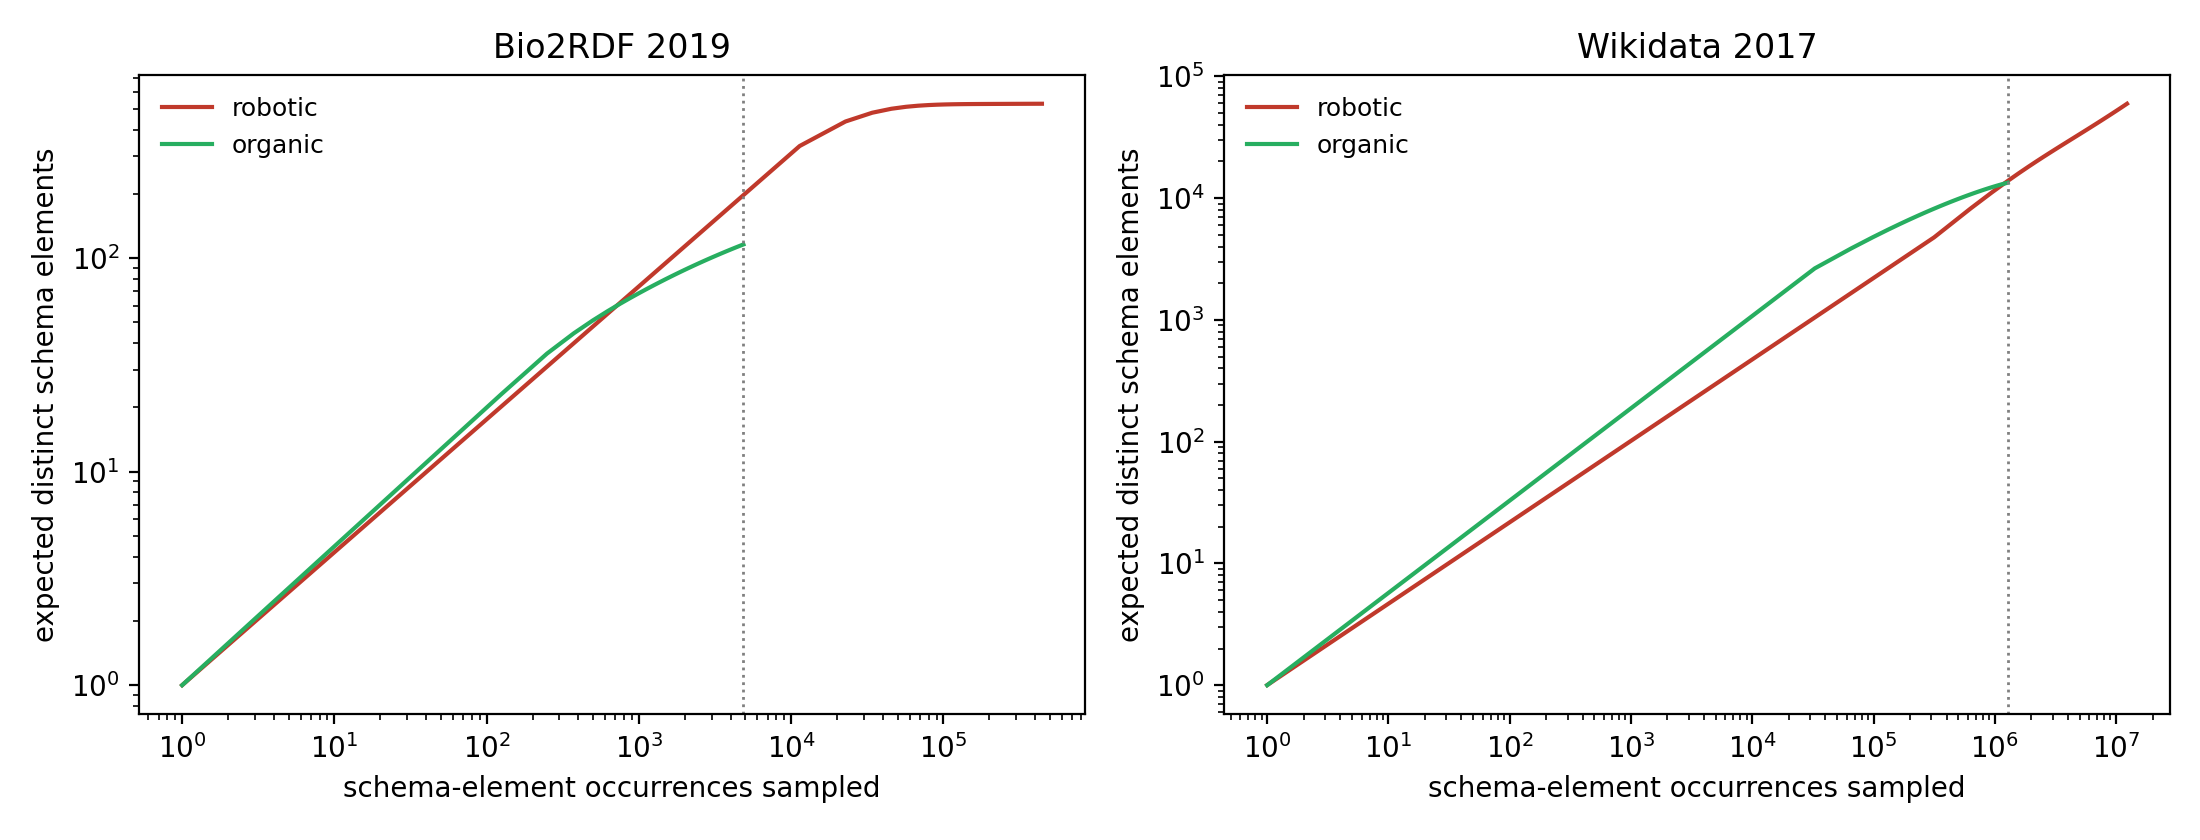
\includegraphics[width=0.95\textwidth]{rarefaction.png}
    \caption{\DIFaddFL{Individual-based rarefaction curves (expected distinct schema elements vs.\ schema-element occurrences sampled, both axes log-scaled) for organic (green) and robotic (red) logs. The dotted line marks the organic log's sampling effort. For Bio2RDF the robotic curve rises well above organic at equal effort; for Wikidata the two curves are close, and organic is in fact richer per occurrence until effort equalizes.}}
    \label{fig:rarefaction}
\end{figure}

\begin{table}[ht]
\centering
\caption{\DIFaddFL{Schema coverage at equal sampling effort. Robotic logs are rarefied down to the number of schema-element occurrences observed in the corresponding organic log.}}
\label{tab:rarefaction}
\begin{tabular}{l|r|r}
\hline
\DIFaddFL{Comparison (equal effort) }& \DIFaddFL{Organic distinct elements (coverage) }& \DIFaddFL{Robotic distinct elements, rarefied (coverage) }\\
\hline
\DIFaddFL{Bio2RDF 2019 ($n=4{,}855$ occ.) }& \DIFaddFL{116 (21.3\%) }& \DIFaddFL{$\approx$208 (38.2\%) }\\
\DIFaddFL{Wikidata 2017 ($n=1{,}279{,}731$ occ.) }& \DIFaddFL{13}\DIFaddendFL ,\DIFdelbeginFL \DIFdelFL{with larger nodes being more frequently used. The color of the nodes follows a gradient from yellow (least used ) }\DIFdelendFL \DIFaddbeginFL \DIFaddFL{394 (12.8\%) }& \DIFaddFL{$\approx$13,846 (13.3\%) }\\
\hline
\end{tabular}
\end{table}

\DIFadd{The two KGs behave oppositely. For }\textbf{\DIFadd{Bio2RDF}}\DIFadd{, even at identical sampling effort the robotic log recovers roughly $1.8\times$ more distinct schema elements than the organic log (208 vs.\ 116; 38.2\% vs.\ 21.3\%), and its rarefaction curve saturates near the full schema. A Monte-Carlo subsampling bootstrap (400 replicates, robotic rarefied to the organic effort of 4}{\DIFadd{,}}\DIFadd{855 occurrences) puts this equal-effort ratio at }\textbf{\DIFadd{1.79$\times$, 95\% CI }[\DIFadd{1.62, 1.96}]} \DIFadd{--- comfortably above 1 --- so robotic clients genuinely exercise a broader part of this small, specialized schema, consistent with automated enumeration or dumping. For }\textbf{\DIFadd{Wikidata}}\DIFadd{, the picture reverses: at equal effort the same bootstrap gives a ratio of only }\textbf{\DIFadd{1.03$\times$, 95\% CI }[\DIFadd{1.02, 1.05}]} \DIFadd{(robotic 13.3\% vs.\ organic 12.8\% of TSE), and at }\emph{\DIFadd{lower}} \DIFadd{effort organic queries are actually richer per occurrence (Figure~\ref{fig:rarefaction}, right). The raw coverage gap in Table~\ref{tab:5} (57\% vs.\ 13\%, i.e.\ $4.4\times$) therefore collapses to a $\sim$3\% difference once effort is equalized: it is almost entirely an artifact of robotic logs being two orders of magnitude larger, not evidence of broader robotic interest. (With $n\,{=}\,1.28$M the tiny residual is statistically distinguishable from 1.0, but its magnitude --- 3\% vs.\ Bio2RDF's 79\% --- is negligible.)
}

\DIFadd{This size dependence is reinforced by how concentrated each log is on once-seen elements (Table~\ref{tab:singletons}). Two thirds of the schema elements counted for }\emph{\DIFadd{Wikidata-robotic-2017}} \DIFadd{are used exactly once; removing these singletons (the elements most exposed to one-off or erroneous uses) drops its coverage from 57.1\% to 18.9\% and shrinks the robotic-to-organic coverage ratio from $4.4\times$ }\DIFaddend to \DIFdelbegin \DIFdel{dark blue (most used ). Similarly,edge thickness and color represent predicate usage, with thinner, light pink edges indicating less usage and thicker, deep purple edges indicating higher usage . Unused schema elements (both nodes and edges) are displayed in gray. }\DIFdelend \DIFaddbegin \DIFadd{$2.0\times$. By contrast, }\emph{\DIFadd{Bio2RDF-robotic-2019}} \DIFadd{has a single singleton: its breadth is exercised repeatedly and is robust. In practical terms, robotic ``coverage'' on a very large KG such as Wikidata largely reflects query volume and a long tail of one-off references, whereas on a compact KG such as Bio2RDF it reflects systematic, repeated traversal of the schema.
}

\begin{table}[ht]
\centering
\caption{\DIFaddFL{Singleton sensitivity. Schema elements used exactly once, and coverage with vs.\ without singletons (2017 logs for Wikidata, 2019 for Bio2RDF).}}
\label{tab:singletons}
\begin{tabular}{l|r|r|r|r}
\hline
\DIFaddFL{Log }& \DIFaddFL{Used elements }& \DIFaddFL{Singletons (\%) }& \DIFaddFL{Coverage }& \DIFaddFL{Coverage w/o singletons }\\
\hline
\DIFaddFL{Wikidata robotic }& \DIFaddFL{59,603 }& \DIFaddFL{39,900 (67\%) }& \DIFaddFL{57.1\% }& \DIFaddFL{18.9\% }\\
\DIFaddFL{Wikidata organic (full) }& \DIFaddFL{13,394 }& \DIFaddFL{3,412 (25\%) }& \DIFaddFL{12.8\% }& \DIFaddFL{9.6\% }\\
\DIFaddFL{Bio2RDF robotic }& \DIFaddFL{529 }& \DIFaddFL{1 (0.2\%) }& \DIFaddFL{97.1\% }& \DIFaddFL{96.9\% }\\
\DIFaddFL{Bio2RDF organic }& \DIFaddFL{116 }& \DIFaddFL{32 (28\%) }& \DIFaddFL{21.3\% }& \DIFaddFL{15.4\% }\\
\hline
\end{tabular}
\end{table}

\paragraph{\textbf{\DIFadd{Validity of the extracted classes.}}} \DIFadd{Because a Wikidata ``class'' is just an item used as the object of }\texttt{\DIFadd{wdt:P31}}\DIFadd{/}\texttt{\DIFadd{wdt:P279}}\DIFadd{, one must ask how many extracted classes are genuine schema rather than uninstantiated or one-off (possibly erroneous) edits. We characterize each class by its }\emph{\DIFadd{support}} \DIFadd{--- the number of times it is the object of }\texttt{\DIFadd{wdt:P31}} \DIFadd{or }\texttt{\DIFadd{wdt:P279}} \DIFadd{in the KG (instances plus subclasses). Of the 103}{\DIFadd{,}}\DIFadd{355 extracted 2017 classes, 42.3\% are instantiated ($\geq 1$ instance), 88.2\% are embedded in the subclass hierarchy, and 30.3\% are }\emph{\DIFadd{singletons}} \DIFadd{(used as a class exactly once) --- the elements most exposed to data glitches. Crucially, }\emph{\DIFadd{querying selects for well-supported classes}}\DIFadd{: among the classes referenced in organic-2017 queries, 72.5\% are instantiated (vs.\ 42.3\% in the universe), the median support is 9 (vs.\ 3), and only 15.8\% are singletons. To check whether even the singleton tail is spurious, we drew a random sample of 100 queried singletons and looked them up: 80\% carry an explicit }\texttt{\DIFadd{wdt:P279}} \DIFadd{(}\emph{\DIFadd{subclass of}}\DIFadd{) statement or a metaclass marker --- i.e.\ they were }\emph{\DIFadd{intentionally}} \DIFadd{modelled as classes --- and manual inspection of the remainder finds mostly genuine but rare concepts and taxa (e.g.\ }\emph{\DIFadd{Quercus velutina}}\DIFadd{, }\emph{\DIFadd{Pinales}}\DIFadd{, }\emph{\DIFadd{ghat}}\DIFadd{) rather than errors; outright noise (e.g.\ a disambiguation item) is rare. The data-glitch risk the metric inherits is therefore real but small, and concentrated in an uninstantiated long tail that actual query demand largely avoids.
}

\subsection{\DIFadd{Organic vs.\ Robotic in the 2013-era Bio2RDF Log}}\label{sec:bio2013}
\DIFaddend The \DIFdelbegin \DIFdel{interactive version of this visualization is available online }\footnote{%DIFDELCMD < \url{https://marmhm.github.io/Schema-usage-graph/ } %%%
}%DIFAUXCMD
\addtocounter{footnote}{-1}%DIFAUXCMD
\DIFdel{. }\DIFdelend \DIFaddbegin \DIFadd{LSQ-derived }\emph{\DIFadd{Bio2RDF-all-2013}} \DIFadd{log is anonymized and cannot be split by user agent. To examine the 2013 era at the same organic/robotic granularity as the rest of the paper, we processed the }\emph{\DIFadd{raw}} \DIFadd{Bio2RDF server access log (the upstream source of LSQ), spanning May 2013--September 2015. It contains 127.2M executed SPARQL requests (HTTP~200), each carrying a user agent and the dataset endpoint (}\texttt{\DIFadd{cu.}\textit{\DIFadd{dataset}}\DIFadd{.bio2rdf.org}}\DIFadd{).
}\DIFaddend 

\DIFaddbegin \DIFadd{The first lesson is about what such a log actually contains (Table~\ref{tab:bio2013comp}): }\textbf{\DIFadd{organic (browser) queries are only 0.09\%}} \DIFadd{of executed traffic. The bulk is machine-generated and, revealingly, much of it is }\emph{\DIFadd{infrastructure}}\DIFadd{: 24\% are Bio2RDF's own Virtuoso engine acting as an HTTP client (federated }\texttt{\DIFadd{SERVICE}} \DIFadd{calls and dereferencing --- 99.6\% of these come from a single host in the hosting institution's network, and their bodies are single-entity label/cross-reference lookups), and a further 22\% is a sustained empty-user-agent crawl from the network of the LSQ project itself, i.e.\ the harvesting that built the public dataset. Any usage statistic computed over the raw log without removing such traffic would largely measure the infrastructure rather than users --- a concrete instance of the example-/tool-contamination concern that any log study must control for.
}

\begin{table}[ht]
\centering
\caption{\DIFaddFL{Composition of the raw 2013--2015 Bio2RDF server log (127.2M executed SPARQL requests) by user-agent class. Genuine human (browser) traffic is 0.09\%; about half of all traffic is the endpoint's own Virtuoso federation/dereferencing or the LSQ harvest.}}
\label{tab:bio2013comp}
\begin{tabular}{l|r}
\hline
\DIFaddFL{User-agent class }& \DIFaddFL{Share of executed requests }\\
\hline
\DIFaddFL{Programmatic tools / libraries (Java, Jena, \ldots) }& \DIFaddFL{49.8\% }\\
\DIFaddFL{Virtuoso-internal (federation / dereferencing) }& \DIFaddFL{24.4\% }\\
\DIFaddFL{LSQ-harvest (sustained empty-UA crawl) }& \DIFaddFL{22.4\% }\\
\DIFaddFL{Search-engine crawlers }& \DIFaddFL{1.7\% }\\
\DIFaddFL{Other / no agent }& \DIFaddFL{1.6\% }\\
\textbf{\DIFaddFL{Organic (browser)}} & \textbf{\DIFaddFL{0.09\% (115}{\DIFaddFL{,}}\DIFaddFL{420)}} \\
\hline
\end{tabular}
\end{table}

\DIFadd{Restricting to the 115}{\DIFadd{,}}\DIFadd{420 organic queries (61}{\DIFadd{,}}\DIFadd{628 unique; 50.3\% syntactically valid --- the rest is the non-SPARQL web spam noted in Section~\ref{s5}), 2013-era organic queries cover }\textbf{\DIFadd{53.6\% of the Bio2RDF schema}} \DIFadd{(167/350 types, 125/195 predicates), exercising the expected biomedical core (}\emph{\DIFadd{drugbank:Drug}}\DIFadd{, }\emph{\DIFadd{omim:Gene}}\DIFadd{/}\emph{\DIFadd{Phenotype}}\DIFadd{, }\emph{\DIFadd{drugbank:Target}}\DIFadd{, }\emph{\DIFadd{kegg:Pathway}}\DIFadd{, }\emph{\DIFadd{pharmgkb:Disease}}\DIFadd{). This is far above the 21.3\% of organic-2019, but the comparison must control for effort: the 2013 organic log has roughly five times as many unique queries. Rarefying both to equal sampling effort (Section~\ref{sec:rarefaction}), organic-2013 recovers 33.7\% vs.\ organic-2019's 21.3\% --- a residual }\textbf{\DIFadd{1.58$\times$}} \DIFadd{difference that is genuine, not a size artifact. The most plausible explanation is architectural: in 2013 Bio2RDF exposed a }\emph{\DIFadd{separate endpoint per dataset}}\DIFadd{, so human exploration spread across the specialized subgraphs, whereas the single unified 2019 endpoint concentrated organic queries on a narrower core. This both removes the paper's earlier inability to split the 2013 log and adds a temporal organic comparison that reinforces the central rarefaction message: raw coverage tracks sampling effort, and only an equal-effort comparison exposes genuine behavioral or architectural differences.
}

\subsection{\DIFadd{What Wikidata Coverage Actually Measures: Class- vs.\ Value-Position Usage}}\label{sec:classvalue}
\DIFadd{A schema-coverage metric implicitly assumes that an element counted as ``used'' is used }\emph{\DIFadd{as schema}}\DIFadd{. For Bio2RDF this holds: its vocabulary classes are never used as property values. For Wikidata it does not, because the same item is routinely referenced as a value (e.g.\ }\texttt{\DIFadd{Q33999}} \emph{\DIFadd{actor}} \DIFadd{as the value of }\texttt{\DIFadd{P106}} \emph{\DIFadd{occupation}}\DIFadd{) rather than as a class. We therefore re-examine the Wikidata results by classifying every entity reference as class-position (object of }\texttt{\DIFadd{wdt:P31}}\DIFadd{/}\texttt{\DIFadd{wdt:P279}}\DIFadd{, or of a path involving them) or value-position (Section~\ref{s3}.2).
}

\DIFadd{Table~\ref{tab:classvalue} shows the split. Among the entities our extraction counts as Wikidata }\emph{\DIFadd{used types}} \DIFadd{(those referenced in queries that are also objects of }\texttt{\DIFadd{wdt:P31}}\DIFadd{/}\texttt{\DIFadd{wdt:P279}} \DIFadd{in the KG), only }\textbf{\DIFadd{70.2\% of organic}} \DIFadd{ones are ever used as a class --- }\textbf{\DIFadd{29.8\% are referenced solely as values}} \DIFadd{--- whereas robotic queries use 92.9\% of their counted types as classes. Weighted by reference volume the contrast narrows (both query types are dominated by value references, since queries fetch values): only $\sim$27--29\% of all type-item references are in class position. Two readings follow. First, the published Wikidata coverage }\emph{\DIFadd{over-counts schema usage}}\DIFadd{, most so for human queries, where roughly a third of the ``used types'' are mis-counted value-items (}\emph{\DIFadd{actor}}\DIFadd{, }\emph{\DIFadd{female}}\DIFadd{, }\emph{\DIFadd{India}}\DIFadd{). Second, this is itself a behavioral signal: humans reference type-items as values, while bots traverse them as classes.
}

\begin{table}[ht]
\centering
\caption{\DIFaddFL{Class- vs.\ value-position usage of the Wikidata ``used types'' (2017). A type is used }\emph{\DIFaddFL{as a class}} \DIFaddFL{only when it is the object of }\texttt{\DIFaddFL{wdt:P31}}\DIFaddFL{/}\texttt{\DIFaddFL{wdt:P279}} \DIFaddFL{(or a path involving them) in a query.}}
\label{tab:classvalue}
\begin{tabular}{l|r|r|r}
\hline
\DIFaddFL{Query type }& \DIFaddFL{\#Used types }& \DIFaddFL{Used as a class }& \DIFaddFL{Value-only }\\
\hline
\DIFaddFL{Wikidata organic 2017 }& \DIFaddFL{12,773 }& \DIFaddFL{8,968 (70.2\%) }& \DIFaddFL{3,805 (29.8\%) }\\
\DIFaddFL{Wikidata robotic 2017 }& \DIFaddFL{58,689 }& \DIFaddFL{54,534 (92.9\%) }& \DIFaddFL{4,155 (7.1\%) }\\
\hline
\end{tabular}
\end{table}

\DIFadd{Beyond the position of reference, comparing query }\emph{\DIFadd{demand}} \DIFadd{against KG }\emph{\DIFadd{supply}} \DIFadd{(instances per class, extracted from the dump) reveals a pronounced inversion (Figure~\ref{fig:mismatch}). The most heavily instantiated Wikidata classes are almost never queried: e.g.\ }\emph{\DIFadd{ravine}} \DIFadd{($\sim$17}{\DIFadd{,}}\DIFadd{000 instances), }\emph{\DIFadd{reef}}\DIFadd{, }\emph{\DIFadd{cairn}}\DIFadd{, }\emph{\DIFadd{qanat}}\DIFadd{, }\emph{\DIFadd{shoal}}\DIFadd{, and (for bots) }\emph{\DIFadd{Wikimedia navigational template}} \DIFadd{($\sim$27}{\DIFadd{,}}\DIFadd{000), }\emph{\DIFadd{protein domain}}\DIFadd{, and }\emph{\DIFadd{microRNA}} \DIFadd{--- all bulk- or bot-imported categories with essentially zero human or robotic class-position demand. Conversely, the genuinely class-queried core is small and intuitive: }\emph{\DIFadd{human}} \DIFadd{(}\texttt{\DIFadd{Q5}}\DIFadd{), }\emph{\DIFadd{city}}\DIFadd{, }\emph{\DIFadd{film}}\DIFadd{, }\emph{\DIFadd{country}}\DIFadd{, }\emph{\DIFadd{painting}} \DIFadd{for organic queries, and }\emph{\DIFadd{human-geographic territorial entity}}\DIFadd{, }\emph{\DIFadd{film}}\DIFadd{, }\emph{\DIFadd{album}}\DIFadd{, }\emph{\DIFadd{church building}}\DIFadd{, }\emph{\DIFadd{book}}\DIFadd{, }\emph{\DIFadd{business}} \DIFadd{for robotic. In other words, the bulk of what Wikidata }\emph{\DIFadd{contains}} \DIFadd{is not what users }\emph{\DIFadd{query}}\DIFadd{, and much of what users query as ``types'' the model does not treat as classes at all.
}

\begin{figure}
    \centering
    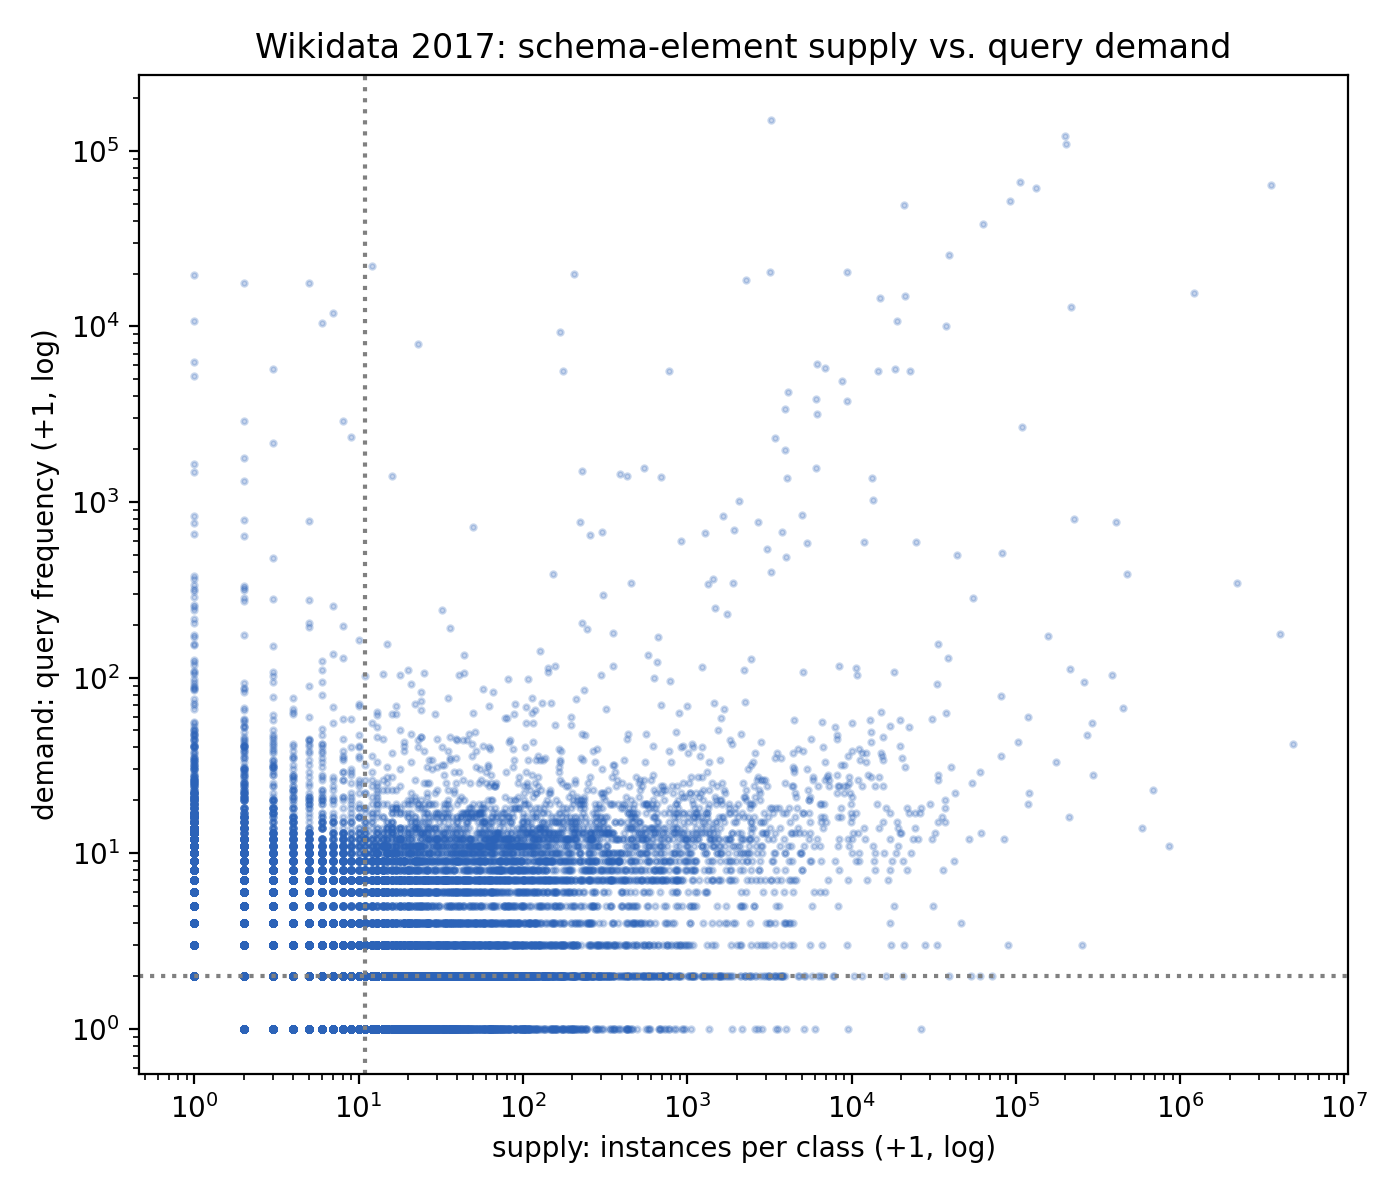
\includegraphics[width=0.6\textwidth]{wd_mismatch.png}
    \caption{\DIFaddFL{Wikidata schema-element supply (instances per class, from the 2017 dump) vs.\ organic query demand (query frequency). Dotted lines mark the high-supply and high-demand thresholds. Heavily instantiated classes (lower right) attract little query demand, while the highest-demand items (upper left) have few or no instances because they are queried as values, not classes.}}
    \label{fig:mismatch}
\end{figure}

\DIFadd{The inversion is not idiosyncratic to individual classes but holds across natural }\emph{\DIFadd{domains}}\DIFadd{. We assigned each class to a top-level domain by walking up its }\texttt{\DIFadd{wdt:P279}} \DIFadd{ancestry to a curated set of anchor classes, and compared each domain's share of KG content (instances) with its share of query demand (Table~\ref{tab:domains}). The pattern is stark: the bulk-imported scientific and bibliographic domains --- }\emph{\DIFadd{taxon}}\DIFadd{, }\emph{\DIFadd{gene/protein}}\DIFadd{, }\emph{\DIFadd{astronomical object}}\DIFadd{, and }\emph{\DIFadd{scholarly publication}} \DIFadd{--- together hold }\textbf{\DIFadd{32\% of all instances but draw only $\sim$5\% of organic demand}} \DIFadd{(}\emph{\DIFadd{taxon}} \DIFadd{alone: 7.6\% of content, 0.4\% of demand). Conversely, the }\emph{\DIFadd{person}} \DIFadd{and }\emph{\DIFadd{organization}} \DIFadd{domains hold 15\% of content but attract }\textbf{\DIFadd{$\sim$39\% of organic demand}}\DIFadd{. The split also sharpens the organic/robotic contrast: human queries concentrate on }\emph{\DIFadd{person}} \DIFadd{(29.8\%, vs.\ 14.4\% for bots), whereas robotic queries are far heavier on }\emph{\DIFadd{scholarly publication}} \DIFadd{(14.3\% vs.\ 2.4\%) and }\emph{\DIFadd{geographic features}} \DIFadd{(21.9\% vs.\ 11.1\%) --- consistent with automated bibliographic and gazetteer harvesting. (The residual ``Other'' bucket carries 17.9\% of organic demand and includes the value-position items of Section~\ref{sec:classvalue}, which have no clean class-domain.)
}

\begin{table}[ht]
\centering
\caption{\DIFaddFL{Content--demand inversion by domain (Wikidata 2017). Each class is assigned to a top-level domain via its }\texttt{\DIFaddFL{wdt:P279}} \DIFaddFL{ancestry; columns give the domain's share of KG content (instances) and of organic / robotic query demand. The ratio is organic-demand-share / supply-share ($<1$ = under-queried relative to content, $>1$ = over-queried).}}
\label{tab:domains}
\begin{tabular}{l|r|r|r|r}
\hline
\DIFaddFL{Domain }& \DIFaddFL{Supply (\% instances) }& \DIFaddFL{Organic (\%) }& \DIFaddFL{Org/supply }& \DIFaddFL{Robotic (\%) }\\
\hline
\DIFaddFL{Taxon / species              }& \DIFaddFL{7.6\%  }& \DIFaddFL{0.4\%  }& \DIFaddFL{0.05 }& \DIFaddFL{0.0\% }\\
\DIFaddFL{Scholarly / publication      }& \DIFaddFL{19.1\% }& \DIFaddFL{2.4\%  }& \DIFaddFL{0.13 }& \DIFaddFL{14.3\% }\\
\DIFaddFL{Gene / protein / biomedical  }& \DIFaddFL{4.9\%  }& \DIFaddFL{1.9\%  }& \DIFaddFL{0.39 }& \DIFaddFL{1.7\% }\\
\DIFaddFL{Astronomical object          }& \DIFaddFL{0.5\%  }& \DIFaddFL{0.3\%  }& \DIFaddFL{0.60 }& \DIFaddFL{0.1\% }\\
\DIFaddFL{Creative work                }& \DIFaddFL{33.1\% }& \DIFaddFL{21.8\% }& \DIFaddFL{0.66 }& \DIFaddFL{23.3\% }\\
\DIFaddFL{Geographic feature           }& \DIFaddFL{16.0\% }& \DIFaddFL{11.1\% }& \DIFaddFL{0.69 }& \DIFaddFL{21.9\% }\\
\DIFaddFL{Person (human/occupation)    }& \DIFaddFL{12.0\% }& \DIFaddFL{29.8\% }& \DIFaddFL{2.48 }& \DIFaddFL{14.4\% }\\
\DIFaddFL{Organization / company       }& \DIFaddFL{3.3\%  }& \DIFaddFL{9.1\%  }& \DIFaddFL{2.76 }& \DIFaddFL{14.0\% }\\
\DIFaddFL{Event                        }& \DIFaddFL{1.2\%  }& \DIFaddFL{5.4\%  }& \DIFaddFL{4.5  }& \DIFaddFL{3.0\% }\\
\DIFaddFL{Other / unclassified         }& \DIFaddFL{2.2\%  }& \DIFaddFL{17.9\% }& \DIFaddFL{---  }& \DIFaddFL{7.2\% }\\
\hline
\end{tabular}
\end{table}

\paragraph{\textbf{\DIFadd{Generality across modeling styles: DBpedia.}}} \DIFadd{A natural objection is that this value-position inflation is an artifact of Wikidata's particular conventions, or simply of its scale, rather than of the item-based modeling style as such. To test this we added a third KG, DBpedia, and ran the same class- vs.\ value-position analysis over its public query log (LSQ~2.0). DBpedia is a useful control: like Bio2RDF it is OWL-style --- its classes are dedicated ontology IRIs (}\texttt{\DIFadd{dbo:}}\DIFadd{) used as the object of }\texttt{\DIFadd{rdf:type}}\DIFadd{/}\texttt{\DIFadd{rdfs:subClassOf}} \DIFadd{--- but like Wikidata it is large, broad, and crowd-curated, so it separates the effect of }\emph{\DIFadd{schema model}} \DIFadd{from that of }\emph{\DIFadd{size and breadth}}\DIFadd{. Across 4.26M distinct executed queries, of the 722 }\texttt{\DIFadd{dbo:}} \DIFadd{classes referenced anywhere, }\textbf{\DIFadd{675 (93.5\%) are used in class position and only 47 (6.5\%) are value-only}} \DIFadd{--- close to Bio2RDF's near-zero and far below Wikidata's 29.8\% for human queries (Table~\ref{tab:generality}). The value-only fraction thus tracks the }\emph{\DIFadd{data model}}\DIFadd{, not KG size: the two OWL-style KGs both keep classes in class position, whereas the item-based Wikidata routinely surfaces type-items as values. The content--demand inversion also recurs on DBpedia: its most heavily instantiated classes (}\emph{\DIFadd{Tenure}}\DIFadd{, $\sim$1.3M instances; }\emph{\DIFadd{WikimediaTemplate}}\DIFadd{, $\sim$223k; }\emph{\DIFadd{MilitaryService}}\DIFadd{; }\emph{\DIFadd{Academic}}\DIFadd{) draw essentially no class-position demand, while queries concentrate on a small intuitive core (}\emph{\DIFadd{Place}}\DIFadd{, }\emph{\DIFadd{Person}}\DIFadd{, }\emph{\DIFadd{Film}}\DIFadd{, }\emph{\DIFadd{Company}}\DIFadd{, }\emph{\DIFadd{MusicalArtist}}\DIFadd{). The phenomena we report are therefore not Wikidata-specific.
}

\begin{table}[ht]
\centering
\caption{\DIFaddFL{Value-position inflation tracks the schema model, not KG size. Among the ontology classes }\emph{\DIFaddFL{referenced in queries}}\DIFaddFL{, the fraction ever used in class position (object of the type/subclass property) vs.\ used only as a value. DBpedia and Bio2RDF are OWL-style; Wikidata is item-based.}}
\label{tab:generality}
\begin{tabular}{l|l|r|r}
\hline
\DIFaddFL{KG (queries) }& \DIFaddFL{Schema model }& \DIFaddFL{Used as a class }& \DIFaddFL{Value-only }\\
\hline
\DIFaddFL{Bio2RDF 2019 (organic) }& \DIFaddFL{OWL classes-with-instances }& \DIFaddFL{$\sim$100\% }& \DIFaddFL{$\sim$0\% (by construction) }\\
\DIFaddFL{DBpedia (all executed) }& \DIFaddFL{OWL ontology (}\texttt{\DIFaddFL{dbo:}}\DIFaddFL{) }& \DIFaddFL{675 (93.5\%) }& \DIFaddFL{47 (6.5\%) }\\
\DIFaddFL{Wikidata 2017 (organic) }& \DIFaddFL{item-based }& \DIFaddFL{8,968 (70.2\%) }& \DIFaddFL{3,805 (29.8\%) }\\
\hline
\end{tabular}
\end{table}

\DIFadd{These observations reframe the coverage results for Wikidata: a single ``schema coverage'' percentage, borrowed from the OWL-style Bio2RDF setting, conflates class usage with value usage on an item-based KG. A faithful figure restricts to class-position references over instantiated classes; the residual --- and more informative --- story is the structural mismatch between a KG's instantiated content and actual query demand, which holds across both modeling styles. We return to the implications in Section~\ref{s5}.
}

\DIFaddend \subsection{Knowledge Graph Usage Patterns }
Thus far, we have introduced a method for calculating SPARQL schema coverage, which quantifies interactions with KGs through SPARQL queries. This measure may provide only a superficial view of KG usage. Knowing that a schema element was queried does not necessarily indicate its frequency of usage or temporal consistency. In this section, we present the results of the methods described in Section \ref{sec:s6}, focusing on the frequency distribution and temporal changes in KG usage. For this analysis, we have used unique queries.

\begin{figure}
    \centering
    
\includegraphics[width=0.9\textwidth]{image10.png} 
    \caption{Frequency distribution of schema elements across datasets (A–M). The datasets include: A) Bio2RDF All log2013\_kg2024, B) Bio2RDF All log2019\_kg2024,  C) Bio2RDF robotic log2019\_kg2024, D) Bio2RDF organic log2019\_kg2024, E) Wikidata organic log2017\_kg2017, F) Wikidata organic log2017\_kg2018,  G) Wikidata robotic log2017\_kg2017, H) Wikidata organic log2017\_kg2017, L) Wikidata robotic log2018\_kg2018, M) Wikidata organic log2018\_kg2018. The plot's color represents it's log type: blue for all logs, red for robotic logs, and green for organic logs. }
     \label{fig:l6}
\end{figure}

\subsubsection{Frequency Distribution of Schema Elements}
As described in Section \ref{sec:s61}, we analyze schema element usage patterns by visualizing the frequency distribution of elements across various intervals of robotic and organic query logs from Bio2RDF and Wikidata. Figure \ref{fig:l6} illustrates this distribution \DIFdelbegin \DIFdel{, where }\DIFdelend \DIFaddbegin \DIFadd{on logarithmic axes: }\DIFaddend the y-axis \DIFdelbegin \DIFdel{represents }\DIFdelend \DIFaddbegin \DIFadd{is }\DIFaddend the normalized monthly \DIFdelbegin \DIFdel{count of schema elements (logarithmic scale), while }\DIFdelend \DIFaddbegin \DIFadd{usage count of each schema element and }\DIFaddend the x-axis \DIFdelbegin \DIFdel{represents the index assigned to each schema element. }\DIFdelend \DIFaddbegin \DIFadd{is the schema-element rank (most- to least-frequently used). Both axes are log-scaled with natural-value tick labels. }\DIFaddend The Bio2RDF contain 545 schema elements, whereas Wikidata 2017 and 2018 include 104,314 and 98,462 elements, respectively. The color scheme distinguishes log types: green represents organic logs, red represents robotic logs, and blue represents all logs (organic and robotic combined). The plots (A–M) exhibit a consistent trend: a sharp decline in schema element usage frequency, suggesting that most schema elements are infrequently used.

Plot A (Bio2RDF All log2013\_kg2024) exhibits a more gradual decline in schema element usage compared to Plot B (Bio2RDF All log2019\_kg2024). Plot C (Bio2RDF robotic log2019\_kg2024) demonstrates a higher maximum frequency, with a log count approaching 4, whereas Plot D (Bio2RDF organic log2019\_kg2024) peaks at around 2. This contrast highlights the greater intensity of schema element usage in Bio2RDF robotic queries.

Plots E and F (Wikidata All organic log2017\_kg2017 and Wikidata All organic log2017\_kg2018) show a similar distribution of schema element usage across two different versions of Wikidata. Both intervals of robotic logs in Wikidata, Plot G and Plot L (Wikidata robotic log2017\_kg2017 and Wikidata robotic log2018\_kg2018), exhibit steep declines in schema element usage, with maximum frequencies exceeding a log count of 6.In contrast, Plot H (Wikidata organic log2017\_kg2017) and Plot M (Wikidata organic log2018\_kg2018) peak around 5, indicating less intensive schema element usage in organic queries.

Across all datasets, both organic and robotic queries display a sharp decline in schema element usage. However, robotic queries exhibit higher initial usage, with greater peak frequencies and broader schema element usage, followed by a steeper decline.

\paragraph{\textbf{Wilcoxon signed-rank test.}}We applied the Wilcoxon signed-rank test, as described in Section \ref{sec:s61}, to assess the consistency in schema element usage frequency between the two intervals of query logs for both Bio2RDF and Wikidata datasets.

For Bio2RDF, comparing Bio2RDF All log2013\_kg2024 with Bio2RDF All log2019\_kg2024 yielded a statistic of 6250.000 (p-value = 0.000), indicating a statistically significant difference in schema element usage between these intervals.

For Wikidata, the Wilcoxon signed‐rank test revealed significant changes in schema element usage frequency over time. Specifically, the comparison of the robotic logs (Wikidata robotic log2017\_kg2017 vs. Wikidata robotic log2018\_kg2018) yielded a test statistic of 126,884,288.500 (p-value = 0.000), while the organic logs (Wikidata organic log2017\_kg2017 vs. Wikidata organic log2018\_kg2018) produced a statistic of 607,273.000 (p-value = 0.000). These findings indicate that schema element usage in Wikidata varied significantly between the examined intervals.

\paragraph{\textbf{Changes in Used Schema Element Ranking}}
Using Equation \ref{eq:4}, introduced in Section \ref{sec:s61}, we computed Spearman's rank correlation and found weak to moderate consistency in schema element usage ranking across datasets. For the Bio2RDF logs (Bio2RDF All log2013\_kg2024 and Bio2RDF All log2019\_kg2024), the correlation coefficient of $\rho = 0.158$ ($p = 0.00497$) indicates a weak positive correlation. However, significant rank changes were observed for individual elements, such as \sloppy  % Allows words to break over lines more easily
\href{http://bio2rdf.org/kegg_vocabulary:Target}{kegg\_vocabulary:Target} (dropped 171 ranks), \href{http://bio2rdf.org/drugbank_vocabulary:group}{drugbank\_vocabulary:group} (dropped 167 ranks), and \href{http://bio2rdf.org/kegg_vocabulary:Disease}{kegg\_vocabulary:Disease} (dropped 165 ranks).

For the Wikidata robotic logs (Wikidata robotic log2017\_kg2017 vs. Wikidata robotic log2018\_kg2018), a correlation coefficient of $\rho = 0.484$ ($p = 0$) suggests a
moderate positive correlation, with notable rank changes for schema elements such as 
\href{http://www.wikidata.org/entity/Q4220917}{film award} (Q4220917) (fell by 458 ranks), 
\href{http://www.wikidata.org/entity/Q2831984}{comic book album} (Q2831984) (fell by 443 ranks), and 
\href{http://www.wikidata.org/entity/Q1667921}{novel series} (Q1667921) (fell by 437 ranks).

For the Wikidata organic logs (Wikidata organic log2017\_kg2017 vs. Wikidata organic log2018\_kg2018), a correlation coefficient ($\rho = 0.571$, $p = 7.46 \times 10^{-167}$) indicates a moderate positive correlation, with extreme rank changes for elements such as 
\href{http://www.wikidata.org/prop/direct/P1811}{P1811} (dropped 212 ranks), 
\href{http://www.wikidata.org/entity/Q811534}{remarkable tree} (Q811534) (rose 200 ranks), and 
\href{http://www.wikidata.org/prop/direct/P1423}{P1423} (dropped 182 ranks).

These rank shifts highlight changes in user interactions with the KG. The weak correlation ($\rho = 0.158$) observed for Bio2RDF may be partially attributed to the 6-year interval. In contrast, the Wikidata logs, which had a one-year interval, showed moderate positive correlations ($\rho = 0.484$ for robotic logs and $\rho = 0.571$ for organic logs). The stronger correlations for Wikidata suggest a more consistent use of schema elements over a shorter time frame.

% To evaluate consistency in the relative rank ordering of the schema element pairs between two intervals, we calculated the concordance index (C-index), as defined in Equation~\ref{eq:5}. 
% For the Bio2RDF logs, comparing the intervals of 2013 and 2019, the concordance index (C-index) was 0.539. This indicates a moderate level of agreement in the relative rank ordering of schema element pairs between these two years. For the Wikidata organic logs, comparing the intervals of 2017 and 2018, the concordance index (C-index) was 0.639, reflecting a slightly higher consistency in the rank ordering of schema elements between the two periods. These results suggest varying degrees of stability in the relative ranking of schema elements across the different datasets and time intervals.

\DIFaddbegin \subsubsection{\DIFadd{Robustness over equal-length intervals}}\label{sec:equalintervals}
\DIFadd{The Wilcoxon and Spearman results above compare only two endpoints (the 2017 and 2018 intervals), so an apparent ``moderate stability'' could be an artifact of which two windows were chosen. To test robustness we exploited the fact that the ICCL/Dresden release segments the organic Wikidata log into consecutive }\emph{\DIFadd{equal-length}} \DIFadd{28-day windows. We analyzed seven such windows spanning 2017-06 to 2018-03, holding the schema universe fixed at the 2017 dump so that differences reflect query }\emph{\DIFadd{behavior}} \DIFadd{rather than schema evolution. Because all windows are the same length, raw counts are already time-normalized.
}

\begin{table}[ht]
\centering
\caption{\DIFaddFL{Organic Wikidata schema coverage over seven consecutive equal-length (28-day) windows, against the fixed 2017 schema universe (TSE${=}104{,}289$). Coverage is stable at $\sim$4\% despite a $4.7\times$ range in query volume.}}
\label{tab:temporaltraj}
\begin{tabular}{l|r|r|r|r}
\hline
\DIFaddFL{Window (28 days) }& \DIFaddFL{\#Queries }& \DIFaddFL{Used types }& \DIFaddFL{Used preds }& \DIFaddFL{Coverage }\\
\hline
\DIFaddFL{2017-06-12 -- 07-09 }& \DIFaddFL{192,330 }& \DIFaddFL{3,559 }& \DIFaddFL{479 }& \DIFaddFL{3.87\% }\\
\DIFaddFL{2017-07-10 -- 08-06 }& \DIFaddFL{200,726 }& \DIFaddFL{3,486 }& \DIFaddFL{505 }& \DIFaddFL{3.83\% }\\
\DIFaddFL{2017-08-07 -- 09-03 }& \DIFaddFL{268,464 }& \DIFaddFL{3,360 }& \DIFaddFL{478 }& \DIFaddFL{3.68\% }\\
\DIFaddFL{2017-12-03 -- 12-30 }& \DIFaddFL{500,339 }& \DIFaddFL{4,269 }& \DIFaddFL{561 }& \DIFaddFL{4.63\% }\\
\DIFaddFL{2018-01-01 -- 01-28 }& \DIFaddFL{600,767 }& \DIFaddFL{3,977 }& \DIFaddFL{518 }& \DIFaddFL{4.31\% }\\
\DIFaddFL{2018-01-29 -- 02-25 }& \DIFaddFL{895,767 }& \DIFaddFL{3,991 }& \DIFaddFL{536 }& \DIFaddFL{4.34\% }\\
\DIFaddFL{2018-02-26 -- 03-25 }& \DIFaddFL{872,555 }& \DIFaddFL{4,300 }& \DIFaddFL{528 }& \DIFaddFL{4.63\% }\\
\hline
\end{tabular}
\end{table}

\DIFadd{Three findings emerge (Table~\ref{tab:temporaltraj}). First, }\emph{\DIFadd{coverage is remarkably stable}} \DIFadd{--- between 3.68\% and 4.63\% --- even though query volume ranges from 192K to 896K across the windows. More queries in a window do not expand coverage, which corroborates the rarefaction result (Section~\ref{sec:rarefaction}) that organic coverage saturates at low sampling effort. Second, }\emph{\DIFadd{rank stability is consistent across the whole trajectory}}\DIFadd{: the consecutive-window Spearman correlation of type frequencies stays in a narrow band ($\rho = 0.47$--$0.51$ for all six adjacent pairs), decaying only mildly to $\rho = 0.44$ over the full $\sim$9-month endpoint gap. The moderate organic stability we reported for the single 2017/2018 pair is therefore not an artifact of those two endpoints --- it holds uniformly window-to-window, with gradual long-range drift. Third, the Wilcoxon signed-rank test on per-type frequency change is }\emph{\DIFadd{not}} \DIFadd{significant for most adjacent windows ($p = 0.08$, $0.38$, $0.91$, $0.19$), with significant shifts only across the December--January boundary ($p = 0.004$ and $p = 1.7{\times}10^{-8}$): usage magnitude is largely stationary month-to-month, punctuated by occasional shifts. Finally, fourteen types appear in the top-50 of }\emph{\DIFadd{every}} \DIFadd{window --- }\emph{\DIFadd{human}}\DIFadd{, }\emph{\DIFadd{city}}\DIFadd{, }\emph{\DIFadd{film}}\DIFadd{, }\emph{\DIFadd{country}}\DIFadd{, }\emph{\DIFadd{book}}\DIFadd{, }\emph{\DIFadd{actor}}\DIFadd{, }\emph{\DIFadd{human settlement}}\DIFadd{, }\emph{\DIFadd{painting}}\DIFadd{, }\emph{\DIFadd{business enterprise}}\DIFadd{, }\emph{\DIFadd{airport}}\DIFadd{, }\emph{\DIFadd{cat}}\DIFadd{, }\emph{\DIFadd{male}}\DIFadd{, }\emph{\DIFadd{female}}\DIFadd{, and }\emph{\DIFadd{politician}} \DIFadd{--- a far stronger demonstration of a persistent ``core'' than the pairwise top-50 overlaps below. Notably, several core members (}\emph{\DIFadd{actor}}\DIFadd{, }\emph{\DIFadd{male}}\DIFadd{, }\emph{\DIFadd{female}}\DIFadd{) are value-position items (Section~\ref{sec:classvalue}), reinforcing that the human-query ``type'' core is partly composed of items the model does not treat as classes.
}

\DIFaddend \subsubsection{Frequent Schema Types}
As described in Section \ref{sec:s62}, we analyze the most frequently queried schema types to identify common elements that persist across different time intervals and log types. Figure \ref{fig:l8} illustrates the top 10 schema types queried across multiple datasets, comparing robotic and organic query logs from Wikidata and Bio2RDF. The x-axis \DIFdelbegin \DIFdel{represents the log-transformed total count of schema usages}\DIFdelend \DIFaddbegin \DIFadd{shows the total usage count on a logarithmic scale (with natural-value tick labels)}\DIFaddend , while the y-axis lists the schema types. In this diagram, colors indicate log types: green for organic logs, red for robotic logs, and blue for all logs (both organic and robotic). Common schema classes across paired datasets are highlighted in bold.


Plot A and Plot B (Bio2RDF All log 2013 vs. 2019) show that four out of the ten schema types—\href{http://bio2rdf.org/omim:Gene}{omim:Gene}, \href{http://bio2rdf.org/wormbase:Gene}{wormbase:Gene}, \href{http://bio2rdf.org/drugbank:Target}{drugbank:Target}, and \href{http://bio2rdf.org/drugbank:Drug}{drugbank:Drug}—remain highly frequent despite a six-year gap between the two intervals. Plot C and Plot D (robotic vs. organic Bio2RDF queries of 2019) share only two common elements: \href{http://bio2rdf.org/drugbank:Drug}{drugbank:Drug} and \href{http://bio2rdf.org/phrmgkb:Variation}{phrmgkb:Variation}.

Plot E and Plot F (Wikidata All organic log 2017 with KG versions of 2017 and 2018) reveal a notable update in schema types, with \href{https://www.wikidata.org/wiki/Q142}{"France (Q142)"} newly classified as a schema type, while the rest of the frequently used schema types remain consistent with those from 2017. Plot G and Plot H (Wikidata robotic vs. organic 2017) share only three common elements: \href{https://www. wikidata.org/wiki/Q5}{"human (Q5)"}, \href{https://www.wikidata.org/wiki/Q11424}{"film (Q11424)"}, and \href{https://www.wikidata.org/wiki/Q515}{"city (Q515)"}. Plot L and Plot M (Wikidata robotic vs. organic 2018) also have three common elements: \href{https://www.wikidata.org/wiki/Q5}{"human (Q5)"}, \href{https://www.wikidata.org/wiki/Q11424}{"film (Q11424)"}, and \href{https://www.wikidata.org/wiki/Q21191270}{"television series episode (Q21191270)"}. Notably, \href{https://www.wikidata.org/wiki/Q5}{"human (Q5)"} and \href{https://www.wikidata.org/wiki/Q11424}{"film (Q11424)"} remain frequent across both 2017 and 2018 for both robotic and organic query types.

The comparison of the top 50 schema types across different intervals and query types further reveals that 24\% of the elements are common between Bio2rdf 2013 and 2019, 42\% overlap between robotic and organic queries in Bio2rdf 2019. For Wikidata, the overlap between robotic and organic queries is 30\% in 2017 and 36\% in 2018, with a 46\% commonality when comparing organic queries across the two years and 32\% common between robotic queries across 2017 and 2018.

Together, the analyses using both the top 10 and top 50 thresholds demonstrate that a core set of schema elements consistently drives query activity across these KGs. This consistency demonstrates the fundamental role of these schema types in shaping user interactions, regardless of temporal or query-type variations. \DIFaddbegin \DIFadd{In practical terms, this stable core is exactly the set that a documentation effort, an autocomplete feature, or a query-recommendation tool for the KG could prioritize with confidence.
}\DIFaddend 

\DIFaddbegin \paragraph{\textbf{\DIFadd{Example-query contamination, measured and bounded.}}} \DIFadd{A natural worry for any log study is that demonstration and example queries inflate apparent usage. We quantified this directly. We matched the full organic log against the Wikidata Query Service example set as it stood in our log period (the 2017-06-30 revision of the examples page: 348 templates, 313 of which we could fingerprint), using a variable- and literal-invariant canonical fingerprint that is robust to variable renaming and label-service boilerplate. Verbatim example runs account for only }\textbf{\DIFadd{2.5\% of unique organic queries and 1.4\% of executions}}\DIFadd{; removing them changes the used-type count by a single element (12,773 to 12,772) and leaves the top-type ranking unchanged. Example traffic is therefore present but does not distort the aggregate coverage or frequency results, and our use of deduplicated (unique-query) counts further limits its influence.
}

\DIFadd{This measurement also corrects a tempting but misleading anecdote. The item \href{https://www.wikidata.org/wiki/Q6581072}{\emph{female} (\texttt{Q6581072})} is referenced in 9,753 unique organic queries; its true counterpart \href{https://www.wikidata.org/wiki/Q6581097}{\emph{male} (\texttt{Q6581097})} is queried less, but not absent (2,931 unique queries) --- a ratio of roughly 3:1, not the ``perfect'' asymmetry one obtains by comparing }\emph{\DIFadd{female}} \DIFadd{against }\texttt{\DIFadd{Q6581080}}\DIFadd{, which is not ``male'' at all but }\emph{\DIFadd{Pirhasan}}\DIFadd{, an administrative quarter in Erzurum, Turkey. The residual female-skew reflects the female-weighting of the example set (its women-focused queries are adapted by users, and so escape verbatim matching) together with genuine interest in gender-gap analyses on Wikidata --- a content signal, not a parsing artifact. This case also illustrates the class-extraction caveat of Section~\ref{s3}.2: }\emph{\DIFadd{female}} \DIFadd{is counted as a ``used type'' only because it is an object of }\texttt{\DIFadd{wdt:P31}}\DIFadd{/}\texttt{\DIFadd{wdt:P279}} \DIFadd{somewhere in the data, even though in queries it functions as a property value, not a class.
}

 \DIFaddend \begin{figure}
    \centering
    
\includegraphics[width=0.8\textwidth]{image7.png} 
    \caption{The most frequent schema types across datasets (A–M). The datasets include: A) Bio2RDF All log2013\_kg2024, B) Bio2RDF All log2019\_kg2024,  C) Bio2RDF robotic log2019\_kg2024, D) Bio2RDF organic log2019\_kg2024, E) Wikidata organic log2017\_kg2017, F) Wikidata organic log2017\_kg2018,  G) Wikidata robotic log2017\_kg2017, H) Wikidata organic log2017\_kg2017, L) Wikidata robotic log2018\_kg2018, M) Wikidata organic log2018\_kg2018. The plot's color represents it's log type: blue for all logs, red for robotic logs, and green for organic logs. Bold labels indicate common schema classes that appear across paired datasets side by side.}
     \label{fig:l8}
\end{figure}

\paragraph{\textbf{Pairwise Schema Type Usage of Bio2RDF.}}

This analysis aims to investigate how pairwise schema type patterns that represent relationships between schema types from different Bio2RDF subgraphs have been used in queries over time. We examine the evolution of this type of federated querying by comparing Bio2RDF query logs from 2013 (log\_2013, covering 17 subgraphs) and 2019 (log\_2019, covering 26 subgraphs), as outlined in Section \ref{sec:s62}.

\DIFdelbegin \DIFdel{The total number of unique pairwise schema type patterns in the Bio2RDF schema was 55 in 2013 and 85 in 2019. However, only 3 out of 55 patterns appeared in queries from log\_2013, whereas in log\_2019, 23 out of 85 patterns were used in queries , indicating a substantial }\DIFdelend \DIFaddbegin \DIFadd{A pairwise pattern here is a query triple that links a type from one subgraph to a type from another via a (typically variable) predicate, i.e., an attempt to join data across datasets. The number of }\emph{\DIFadd{distinct}} \DIFadd{cross-subgraph join patterns observed in queries rose from }\textbf{\DIFadd{3 in log\_2013 to 22 in log\_2019}} \DIFadd{--- roughly a sevenfold }\DIFaddend increase in federated querying over time. \DIFaddbegin \DIFadd{We report this as a count rather than a fraction of ``possible'' patterns: the space of possible cross-subgraph joins is large (the schema exhibits 430 directed cross-subgraph type-to-type edges across 26 subgraphs) and, because observed joins use variable predicates rather than specific schema edges, a ``used-out-of-possible'' ratio would compare two different notions. The robust and reproducible quantity is the increase in distinct observed join patterns.
}\DIFaddend 

Figure \ref{fig:l7} presents a heatmap illustrating the pairwise schema type usage across Bio2RDF subgraphs for log\_2013 and log\_2019. The results highlight a significant increase in the diversity of dataset integration in 2019 relative to 2013. This shift reflects broader advancements in data accessibility and integration practices within the bioinformatics community. The observed increase is likely attributable to the adoption of a single query endpoint for all datasets in 2019, which improved accessibility compared to the multiple endpoints used in 2013.

\begin{figure}
    \centering
    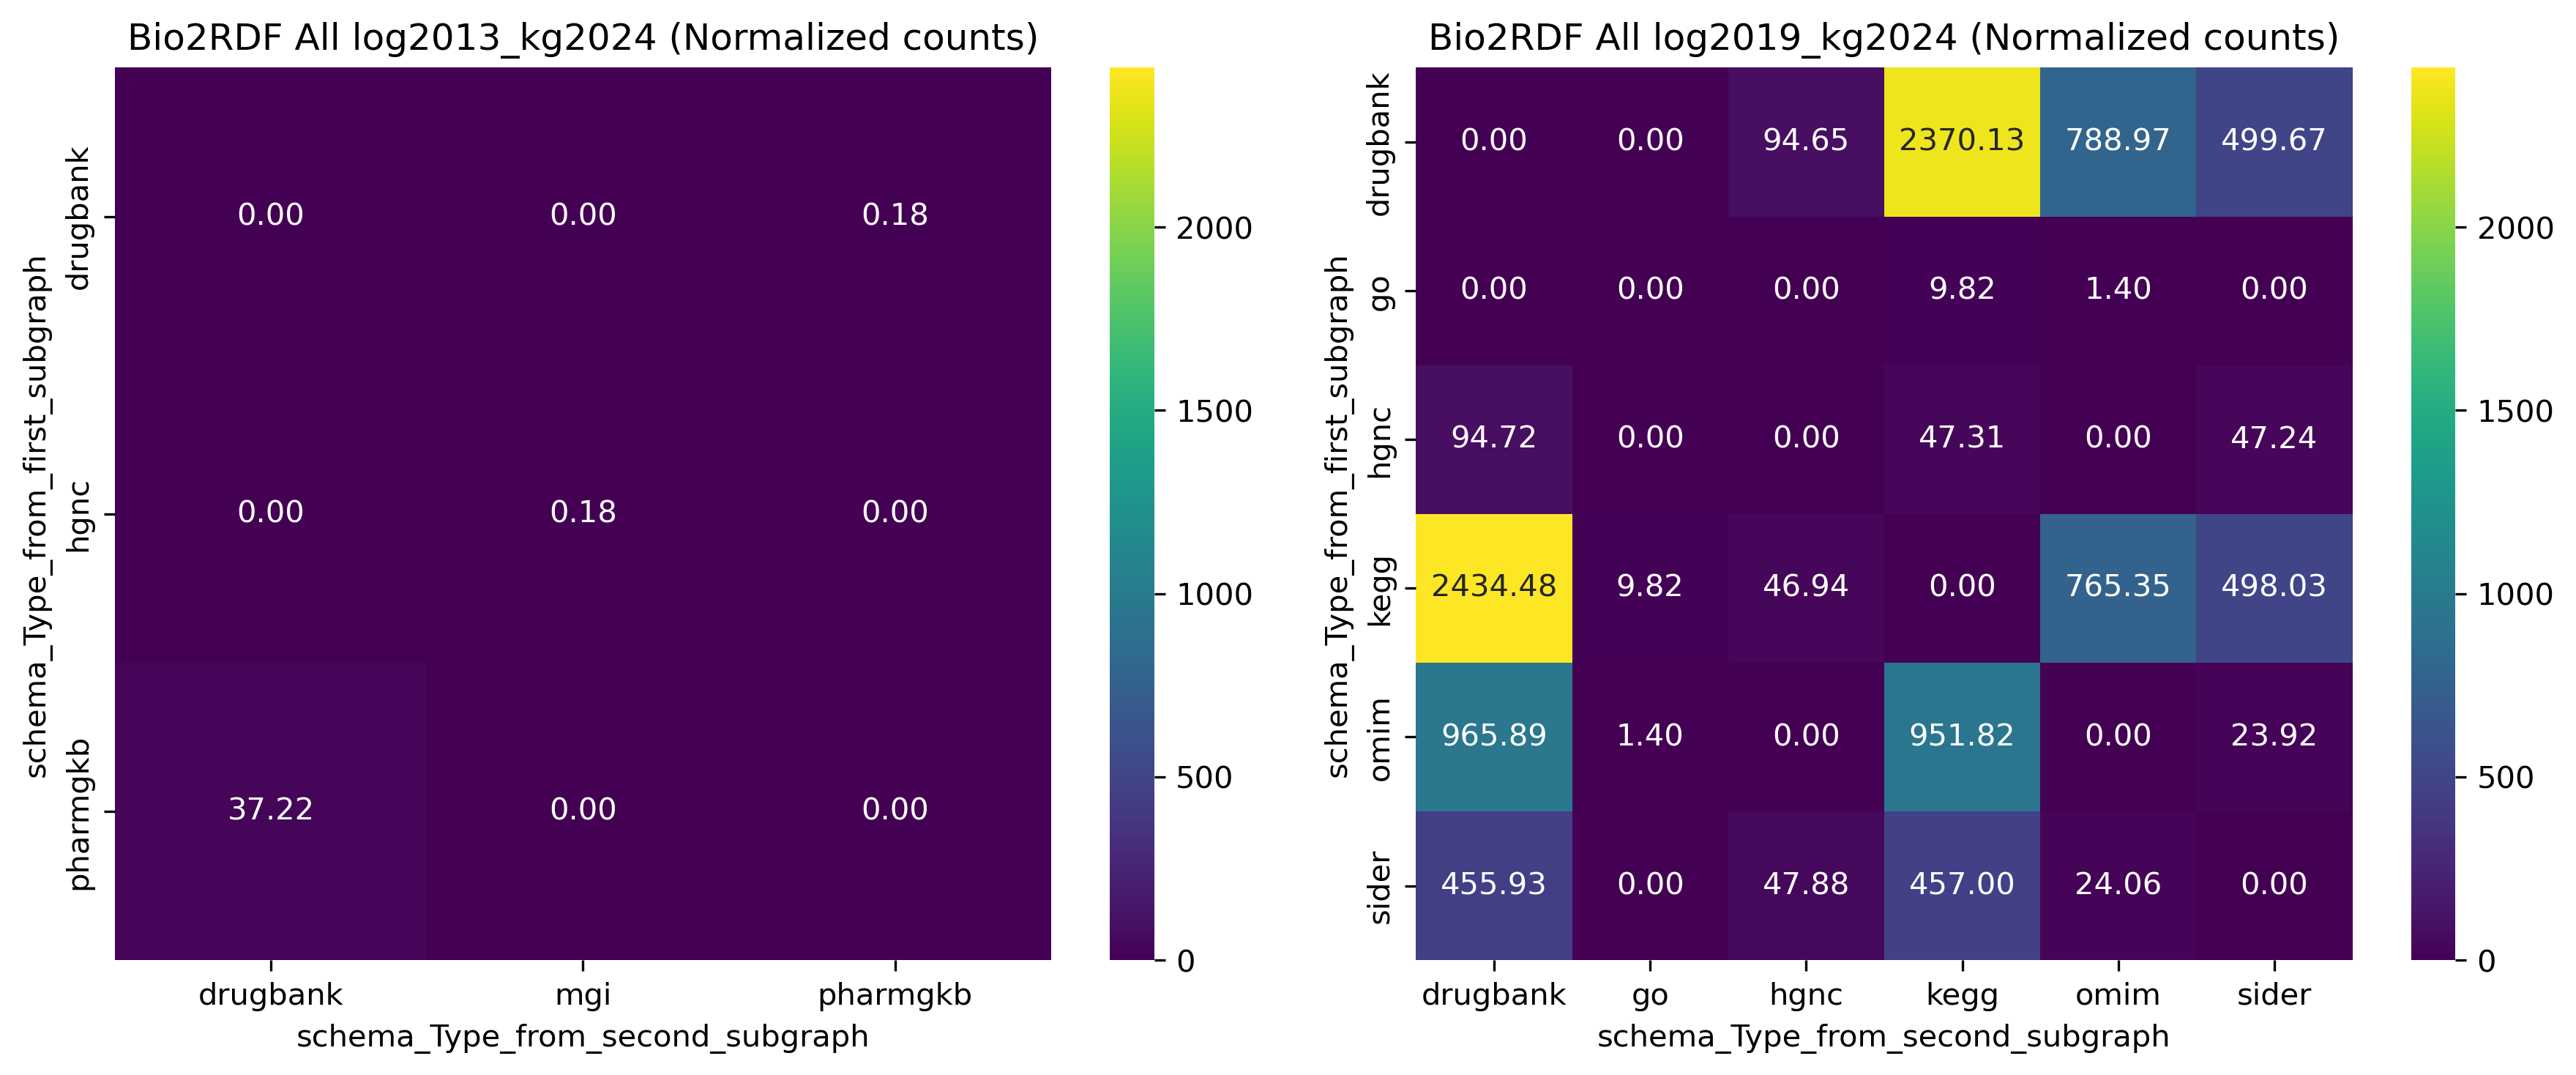
\includegraphics[width=0.8\textwidth]{image24.png} 
    \caption{Heatmap of the pairwise co-occurrence of schema types from two different subgraphs of log 2013 vs. 2019
}
     \label{fig:l7}
\end{figure}

Figure \ref{fig:l9} presents an overview of the usage metadata generated by the proposed method. This approach processes SPARQL queries and KGs to produce usage metadata. The extracted metadata includes SPARQL schema coverage, the schema elements used, their associated usage frequencies, and the generated schema for the respective KGs. The metadata for each dataset is available online for download\footnote{\url{https://github.com/MaastrichtU-IDS/KG_usage_metadata/tree/main/metadata-files}} in CSV and RDF formats.

\begin{figure}
    \centering
    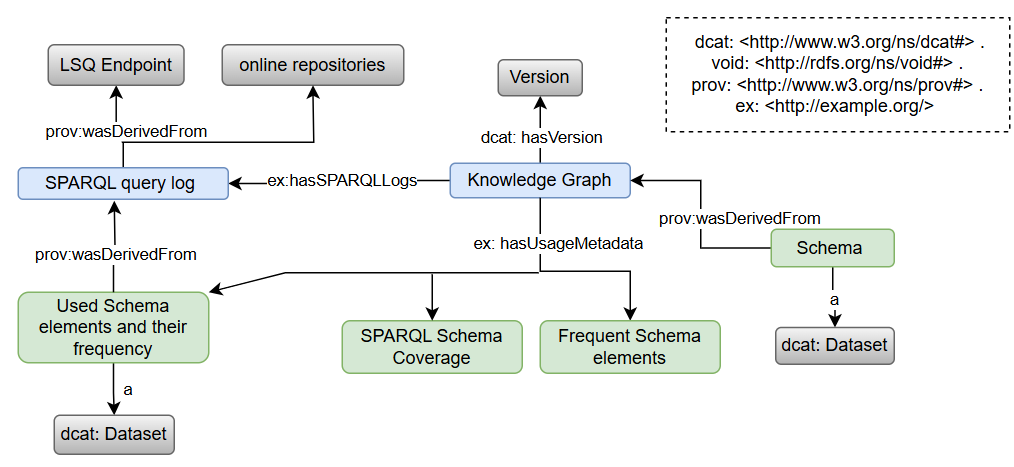
\includegraphics[width=0.8\textwidth]{image16.png} 
    \caption{Usage metadata model
}
    \label{fig:l9}
\end{figure}


\DIFaddbegin \subsection{\DIFadd{Utility: Usage Metadata Forecasts Demand Better Than KG Content}}\label{sec:utility}
\DIFadd{The preceding analyses point to a concrete application: a type-suggestion (autocomplete) feature for a query builder, of the kind a KG maintainer might deploy. We evaluate it as a }\emph{\DIFadd{forecasting}} \DIFadd{task to test whether the usage metadata is actually useful. We rank Wikidata schema types by their class-position usage frequency in the }\emph{\DIFadd{early-2017}} \DIFadd{organic logs (the ``training'' period), and measure what fraction of the class-type demand in the }\emph{\DIFadd{2018}} \DIFadd{organic log (the ``test'' period, $\sim$8 months later) is captured by the top-$k$ suggestions. As a content-based baseline we rank the }\emph{\DIFadd{same}} \DIFadd{types instead by KG }\emph{\DIFadd{supply}} \DIFadd{(instances per class, from the 2017 dump). Following the rest of our frequency analysis (Section~\ref{s4}), demand is computed over unique (deduplicated) queries, so that a single heavily repeated example or tool query cannot dominate the evaluation.
}

\begin{table}[ht]
\centering
\caption{\DIFaddFL{Forecasting utility: \% of 2018 organic class-type demand (deduplicated) captured by the top-$k$ suggested types, ranked by past (2017) usage vs.\ by KG supply (instances/class). Usage metadata transfers across time and outperforms the content-based ranking at every $k$.}}
\label{tab:utility}
\begin{tabular}{r|r|r}
\hline
\DIFaddFL{Top-$k$ suggestions }& \DIFaddFL{Ranked by past usage }& \DIFaddFL{Ranked by KG supply }\\
\hline
\DIFaddFL{10   }& \DIFaddFL{40.3\% }& \DIFaddFL{32.1\% }\\
\DIFaddFL{50   }& \DIFaddFL{54.1\% }& \DIFaddFL{42.3\% }\\
\DIFaddFL{100  }& \DIFaddFL{61.7\% }& \DIFaddFL{49.0\% }\\
\DIFaddFL{500  }& \DIFaddFL{75.7\% }& \DIFaddFL{62.5\% }\\
\DIFaddFL{1000 }& \DIFaddFL{79.9\% }& \DIFaddFL{68.1\% }\\
\hline
\end{tabular}
\end{table}

\DIFadd{Figure~\ref{fig:utility} and Table~\ref{tab:utility} show the result. A list of just the 50 most-used types, learned from 2017, covers }\textbf{\DIFadd{54\%}} \DIFadd{of the distinct-query type demand eight months later, rising to 80\% at top-1000 --- usage metadata transfers across time well enough to drive a real feature. The content-based ranking is markedly worse: its top-50 covers only }\textbf{\DIFadd{42\%}}\DIFadd{, and it must offer }\textbf{\DIFadd{148 suggestions ($3\times$ as many)}} \DIFadd{to match what the usage ranking achieves with 50. The reason is the content--demand inversion of Section~\ref{sec:classvalue}: the highest-supply classes are bulk- and bot-imported categories (}\emph{\DIFadd{scholarly article}}\DIFadd{, }\emph{\DIFadd{Wikimedia category}}\DIFadd{, }\emph{\DIFadd{taxon}}\DIFadd{, }\emph{\DIFadd{disambiguation page}}\DIFadd{, }\emph{\DIFadd{Wikimedia template}}\DIFadd{, }\emph{\DIFadd{gene}}\DIFadd{, }\emph{\DIFadd{protein}}\DIFadd{) that humans rarely query, so a content-ranked tool squanders its top slots, whereas the usage-ranked list surfaces the intuitive core (}\emph{\DIFadd{human}}\DIFadd{, }\emph{\DIFadd{film}}\DIFadd{, }\emph{\DIFadd{city}}\DIFadd{, }\emph{\DIFadd{country}}\DIFadd{, }\emph{\DIFadd{human settlement}}\DIFadd{, }\emph{\DIFadd{university}}\DIFadd{, }\emph{\DIFadd{business}}\DIFadd{). This is direct evidence that the usage metadata we generate has predictive value that KG content statistics alone do not, and it makes concrete the documentation- and autocomplete-prioritization argument of Section~\ref{sec:equalintervals}. The advantage is well outside sampling noise: a query-level bootstrap (2}{\DIFadd{,}}\DIFadd{000 resamples of the 185}{\DIFadd{,}}\DIFadd{443 test queries) gives 95\% confidence intervals of about $\pm$0.5 points on each coverage value, and the usage-minus-supply gap is positive at every list length --- e.g.\ $+11.8$ points at top-50 (95\% CI $[11.2, 12.4]$) and $+11.8$ at top-1000 ($[11.3, 12.4]$).
}

\begin{figure}
    \centering
    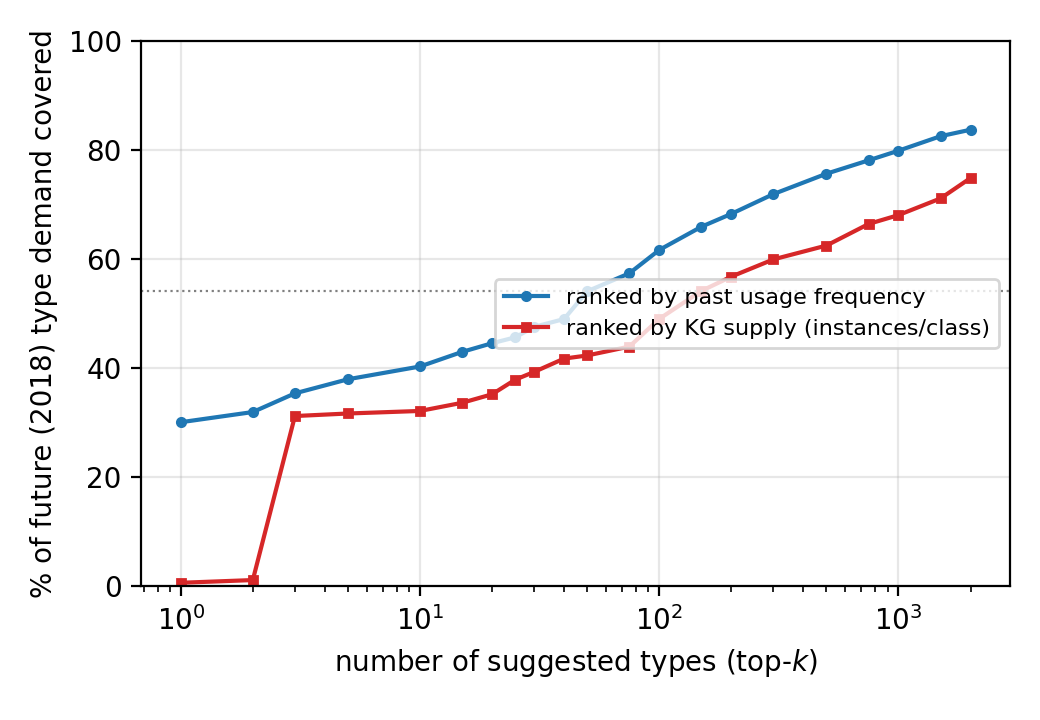
\includegraphics[width=0.62\textwidth]{utility_autocomplete.png}
    \caption{\DIFaddFL{Forecasting future query demand with usage metadata. Each curve shows the percentage of 2018 organic class-type demand (deduplicated) covered by the top-$k$ suggested types, when types are ranked by their 2017 usage frequency (blue) vs.\ by KG supply in instances per class (red). The usage ranking dominates at every list length; the dotted line marks its top-50 coverage.}}
    \label{fig:utility}
\end{figure}

\DIFaddend \section{Discussion}\label{s5}
In this study, we analyzed SPARQL query logs to explore how users interact with knowledge graphs (KGs) by addressing two key questions: (1) How can we quantify the usage of a KG? and (2) Do frequency distribution and ranking analyses of used KG elements reveal usage patterns over different log intervals or across organic (human-driven) and robotic (bot-driven) query types? We applied the proposed method to the both robotic and organic query logs from Bio2RDF and Wikidata, uncovering several patterns in schema element usage.

To quantify the overall usage of a KG, we introduced the \DIFdelbegin \DIFdel{metric of SPARQL schema converge}\DIFdelend \DIFaddbegin \DIFadd{SPARQL schema coverage metric}\DIFaddend , which measures the proportion of schema elements \DIFdelbegin \DIFdel{in a KG that are queried. Our analysis of schema coverage revealed marked differences }\DIFdelend \DIFaddbegin \DIFadd{that are explicitly referenced in queries. Raw coverage differs markedly }\DIFaddend between robotic and organic \DIFdelbegin \DIFdel{queries. Robotic queries exhibited high schema coverage (}\DIFdelend \DIFaddbegin \DIFadd{logs (robotic }\DIFaddend 97\% for Bio2RDF and 60\% for Wikidata\DIFdelbegin \DIFdel{) indicating }\DIFdelend \DIFaddbegin \DIFadd{; organic 21\% and 14\%), which might suggest }\DIFaddend that automated processes \DIFdelbegin \DIFdel{tend to }\DIFdelend \DIFaddbegin \DIFadd{simply }\DIFaddend access a broader range of \DIFdelbegin \DIFdel{schema elements. In contrast, organic queries showed much lower coverage (21\% for }\DIFdelend \DIFaddbegin \DIFadd{the schema. However, robotic and organic logs also differ in size by up to two orders of magnitude, so raw coverage conflates breadth of interest with sheer query volume. The size-controlled rarefaction analysis (Section~\ref{sec:rarefaction}) disentangles the two, and the conclusion is KG-dependent rather than a blanket statement about ``machine vs.\ human'' querying. For }\DIFaddend Bio2RDF\DIFdelbegin \DIFdel{and 14\% for Wikidata )}\DIFdelend \DIFaddbegin \DIFadd{, robotic logs cover roughly $1.8\times$ more of the schema than organic logs }\emph{\DIFadd{even at equal sampling effort}}\DIFadd{, so the broader robotic footprint there is a genuine behavioral difference (systematic, repeated traversal of a compact, specialized schema). For Wikidata, the gap essentially vanishes at equal effort, and organic queries are even richer per query at small samples; the large raw gap is mostly a volume artifact, amplified by a long tail of one-off references (two thirds of robotic Wikidata elements are used exactly once). The practical lesson is that schema coverage must be interpreted relative to sampling effort and to KG scale, and that ``robotic queries cover more'' holds for a small specialized KG but not for a very large one.
}

\DIFadd{A further difference between the two query types is }\emph{\DIFadd{syntactic}}\DIFadd{, and it reinforces the organic/robotic distinction on an axis independent of schema breadth. In the Bio2RDF 2019 logs, robotic queries are almost entirely well-formed}\DIFaddend , \DIFdelbegin \DIFdel{suggesting that human users focus on a smaller subset of the schema elements. These findings indicate distinct interaction patterns between machine-driven and user-driven }\DIFdelend \DIFaddbegin \DIFadd{standards-compliant SPARQL (about 99.5\% of unique robotic queries parse), whereas organic logs are far noisier: a large fraction of unique organic entries are not valid SPARQL at all but injected non-SPARQL text (e.g., blog-comment spam submitted to the public endpoint), and the genuinely non-standard queries that remain---using Virtuoso extensions such as }\texttt{\DIFadd{bif:contains}} \DIFadd{(full-text search), }\texttt{\DIFadd{OPTION}}\DIFadd{, and the }\texttt{\DIFadd{LIKE}} \DIFadd{operator---originate overwhelmingly from organic (human, web-form) traffic rather than from automated clients. In other words, the vendor-specific full-text and option syntax is a human behavior here, not a robotic one. This also cautions that ``valid query'' counts are sensitive to both log hygiene (non-SPARQL contamination of organic logs) and to engine-specific syntax; we verified that the validity rate itself is not an artifact of the chosen parser, since three independent SPARQL~1.1 parsers (a strict grammar, the parser used here, and a Rust engine) agree on validity for 98--99\% of }\DIFaddend queries.

Beyond coverage, we observed a pronounced long-tail distribution in the frequency of schema element usage in both datasets. While a few schema elements are queried very frequently, the vast majority are rarely used. This long-tail phenomenon is significant because it demonstrates that only a limited set of elements captures most of the user attention, despite the overall diversity in accessed elements. Although schema coverage and usage frequency analyses capture different dimensions of query behavior (i.e., the breadth of elements accessed versus the extent of their usage), they together provide a comprehensive view of usage patterns without implying a direct causal relation between them.

We computed Spearman’s rank correlations based on the frequency rankings of common schema elements in dataset pairs. Over a longer time span (e.g., Bio2RDF All logs: 2013 vs. 2019), the weak correlation suggests shifting rankings over time. In contrast, moderate correlation in shorter intervals of Wikidata robotic logs (2017 vs. 2018) and Wikidata organic logs (2017 vs. 2018), indicates greater consistency in the near term.

Focusing on the most frequently queried schema types, our findings reveal a dual pattern in both the top 10 and top 50 elements. In the top 10 analysis, a small stable core, typically comprising 2 to 4 elements, appears consistently across different datasets, time intervals, and query types, while the remaining elements tend to vary. In the top 50 frequent elements, we observe an overlap of 24\% to 46\% common elements across different comparisons. This indicates that although a core set of schema elements remains persistently frequent (likely due to their fundamental role or inherent relevance), the majority of frequently queried elements are variable, reflecting evolving user interests or updates in data structures. Importantly, the persistent core can be leveraged in KG documentation and design, ensuring that these key elements are prioritized and optimized to better serve user needs.

% Taken together, these findings provide a nuanced view of KG usage patterns. Both organic and robotic queries exhibit a long-tail distribution in schema element usage; however, robotic queries access a broader range of elements, while organic queries concentrate on a smaller subset. Recognizing this distinction is important because it reveals that, despite similar overall distributions, the type of query (automated vs. human-driven) influences the breadth of schema elements used. Furthermore, the presence of a stable core in the top 10—coupled with substantial variability in the remaining elements—and the Spearman’s rank correlation results highlight a dual pattern of stability and evolution in KG usage. Short-term consistency exists among the most frequently queried elements, while longer time spans witness more substantial reordering in element popularity. These insights offer valuable perspectives for optimizing knowledge graph design and query strategies to better cater to diverse user needs.

In addition, the pairwise schema \DIFdelbegin \DIFdel{element }\DIFdelend \DIFaddbegin \DIFadd{type }\DIFaddend co-occurrence analysis in Bio2RDF reveals that \DIFdelbegin \DIFdel{while only }\DIFdelend \DIFaddbegin \DIFadd{the number of distinct cross-subgraph join patterns observed in queries increased from }\DIFaddend 3 \DIFdelbegin \DIFdel{out of 55 unique pairwise schema type patterns were observed in }\DIFdelend \DIFaddbegin \DIFadd{in }\DIFaddend the 2013 logs \DIFdelbegin \DIFdel{, this number increased to 23 out of 85 }\DIFdelend \DIFaddbegin \DIFadd{to 22 }\DIFaddend in the 2019 logs. This substantial increase in federated querying indicates an enhanced emphasis on integrating multiple datasets over time, likely driven by improved accessibility, such as the shift from multiple query endpoints in 2013 to a unified endpoint in 2019. These results demonstrate the importance of designing KGs that support robust federated query capabilities, especially in data-driven fields like bioinformatics.

In conclusion, the findings offer a detailed understanding of KG usage patterns and present valuable guidance for refining KG design and query strategies to better address user needs.

This study \DIFdelbegin \DIFdel{faces two main limitationswhen comparing Bio2RDF and Wikidata. First, the }\DIFdelend \DIFaddbegin \DIFadd{has several limitations, which also point to future work.
}

\emph{\DIFadd{Comparability of the two KGs.}} \DIFadd{The }\DIFaddend log collection periods differ \DIFdelbegin \DIFdel{significantly: }\DIFdelend \DIFaddbegin \DIFadd{(}\DIFaddend Bio2RDF \DIFdelbegin \DIFdel{logs span nearly }\DIFdelend \DIFaddbegin \DIFadd{$\sim$}\DIFaddend 30 months \DIFdelbegin \DIFdel{, whereas Wikidata logs cover only }\DIFdelend \DIFaddbegin \DIFadd{vs.\ Wikidata $\sim$}\DIFaddend 9 months\DIFdelbegin \DIFdel{. The limited duration of the Wikidata logs constrains our ability to fully assess long-term usage patterns. A potential avenue for future research is to conduct a direct comparison using equivalent time windows (e.g., nine-month intervals for both KGs) .
Second, there is a substantial difference in scale between the two KGs, as Wikidata’s schema is approximately 200 times larger than }\DIFdelend \DIFaddbegin \DIFadd{) and the schemas differ in scale by roughly two orders of magnitude. We mitigate the first with time-normalized counts and the second by reporting coverage primarily within each KG and by the size-controlled rarefaction analysis; nonetheless, cross-KG coverage percentages should not be read as a direct ranking. For the within-Wikidata temporal comparison we additionally verified the two-endpoint result against seven consecutive equal-length (28-day) windows (Section~\ref{sec:equalintervals}), confirming that coverage ($\sim$4\%) and rank stability ($\rho \approx 0.47$--$0.51$) are not artifacts of the chosen endpoints. Direct comparison across KGs of similar scale remains valuable future work.
}

\emph{\DIFadd{Schema coverage does not transfer cleanly from an OWL-style KG to an item-based one.}}
\DIFadd{This is the study's most consequential lesson, and it emerged from extending a metric
designed for }\DIFaddend Bio2RDF \DIFdelbegin \DIFdel{’s. This disparity naturally affects usage metrics such as schema coverage and frequency distributions.
Future research should consider comparing datasets of similar scale to better account for these differences}\DIFdelend \DIFaddbegin \DIFadd{to Wikidata. In Bio2RDF, classes and predicates are OWL-style
vocabulary terms and ``coverage'' is well defined. In Wikidata there is no formal
class/instance separation; ``classes'' are ordinary items, and --- as Section~\ref{sec:classvalue}
shows --- a large share of the items counted as queried types (about 30\% in human
queries) are referenced only as property }\emph{\DIFadd{values}}\DIFadd{, never as classes. A single
coverage percentage therefore conflates value usage with schema usage, and the Bio2RDF
and Wikidata figures are not directly comparable: the lower Wikidata coverage is partly
definitional, not purely behavioral. For item-based KGs, a faithful usage measure must
(i) separate class-position from value-position references and (ii) restrict to
instantiated classes. The content--demand inversion (Section~\ref{sec:classvalue}, Figure~\ref{fig:mismatch})
sharpens the point: Wikidata's most heavily instantiated classes --- bulk- and
bot-imported geographic, biological, and structural categories --- attract almost no
query demand, while demand concentrates on a small, intuitive class core and on items
queried as values. This also refines the organic/robotic contrast: human queries reference
type-items as values far more than bots do (which traverse them as classes), so human
``coverage'' is the more inflated of the two. A third KG, DBpedia, isolates the cause:
it is as large and broad as Wikidata but OWL-style like Bio2RDF, and only 6.5\% of its
queried classes are value-only (Table~\ref{tab:generality}), with the same content--demand
inversion (heavily instantiated }\emph{\DIFadd{Tenure}}\DIFadd{/}\emph{\DIFadd{WikimediaTemplate}} \DIFadd{unqueried; demand on
}\emph{\DIFadd{Place}}\DIFadd{/}\emph{\DIFadd{Person}}\DIFadd{/}\emph{\DIFadd{Film}}\DIFadd{). Value-position inflation therefore follows the
}\emph{\DIFadd{modeling style}}\DIFadd{, not KG size or breadth, and the inversion generalizes across both styles.
Residual caveats remain --- }\texttt{\DIFadd{wdt:P279}}
\DIFadd{has subproperties we do not follow, and a principled, instance-aware notion of ``class''
for Wikidata is an open problem \mbox{%DIFAUXCMD
\cite{brasileiro2016applying,piscopo2018who,patelschneider2024class}
}\hskip0pt%DIFAUXCMD
--- but the broader message is that usage metrics must be matched to a KG's modeling style.
}

\emph{\DIFadd{Explicit reference vs.\ effective usage.}} \DIFadd{We count a schema element as used when it is explicitly written in a query. This is the right notion for documentation, interface, and deprecation decisions, but it does not capture the subclasses and subproperties that a property path (e.g.\ }\texttt{\DIFadd{wdt:P31/wdt:P279*}}\DIFadd{) traverses at evaluation time and that also contribute to answers. As we show in Section~\ref{s3}.4, a naive closure-based notion is in fact }\emph{\DIFadd{ill-behaved}} \DIFadd{on an item-based KG: because users occasionally anchor }\texttt{\DIFadd{wdt:P279*}} \DIFadd{at near-root classes such as }\emph{\DIFadd{entity}}\DIFadd{, crediting the full subclass closure would mark $\sim$62\% of all Wikidata classes as ``used,'' driven by a handful of queries. A useful effective-usage measure would therefore need to attribute usage }\emph{\DIFadd{partially}} \DIFadd{(e.g.\ weighting by how many traversed elements actually contribute answers, or capping anchor generality) rather than crediting the whole closure; designing such a measure is a natural and substantial extension.
}

\emph{\DIFadd{Example-query contamination and weighting.}} \DIFadd{``Organic'' logs can be contaminated by demonstration and example queries. We measured this directly against the period's Wikidata Query Service example set (Section~\ref{sec:equalintervals}'s frequent-types discussion): verbatim example runs are only $\sim$1.4\% of executions and do not change the coverage or top-type results. This is a lower bound --- it does not capture example queries that users }\emph{\DIFadd{adapt}} \DIFadd{before running (e.g.\ swapping the occupation or class in a template), which a fuzzier, subpattern-based matcher could estimate. Complementing our deduplicated (intent-diversity) counts with volume-weighted counts, and detecting adapted-example traffic, would further sharpen the behavioral interpretation.
}

\subsection{\DIFadd{Implications for practitioners}}\label{sec:implications}
\DIFadd{Beyond the measurement contributions, our results translate into three concrete recommendations for KG maintainers. }\textbf{\DIFadd{(1) Do not rank or compare KGs by a single ``schema coverage'' number.}} \DIFadd{On an item-based KG the figure conflates class usage with value usage and is dominated by a barely-instantiated long tail; a faithful report separates class-position from value-position references and restricts to instantiated classes (Section~\ref{sec:classvalue}). }\textbf{\DIFadd{(2) Drive documentation, interface, and deprecation decisions from usage rather than from content volume.}} \DIFadd{The content--demand inversion means the most-instantiated classes are often the least queried; our forecasting experiment (Section~\ref{sec:utility}) shows a usage-ranked suggestion list captures markedly more future demand than a content-ranked one of equal length, and that the queried core is small, intuitive, and temporally stable (Section~\ref{sec:equalintervals}) --- exactly the set worth documenting and surfacing in autocomplete, while the persistently-unqueried, uninstantiated tail is where deprecation review can focus. }\textbf{\DIFadd{(3) Separate the human signal from the bot signal, and guard against example-query contamination.}} \DIFadd{The organic and robotic logs differ not only in volume but in what and how they query; size-controlled analysis (Section~\ref{sec:rarefaction}) is needed before reading a coverage gap as behavioral, and demonstration queries can masquerade as organic demand and must be detected before usage statistics are trusted for human-facing decisions}\DIFaddend .

% Another avenue for further exploration lies in addressing the semantic gap between user queries and KG content. To investigate how well current KGs align with user needs, identifying potential mismatches and opportunities to adjust KG schema to improve responsiveness to real-world queries. This could involve developing metrics to quantify the alignment between user intent and KG schema.


\section{Conclusion}\label{s6}
This study introduces a novel approach for analyzing SPARQL query logs to gain deeper insights into user interactions with knowledge graphs (KGs). To identify usage patterns, we introduce the SPARQL schema coverage metric and conduct frequency distribution and ranking analyses of queried KG elements across different log intervals and both organic and robotic query types from Bio2RDF and Wikidata.
The findings reveal that \DIFdelbegin \DIFdel{, while }\DIFdelend both query types in both datasets exhibit a long-tail distribution in schema element usage\DIFdelbegin \DIFdel{, robotic queries access a broader range of elements (60–97\%) , whereas organic queries focus on a narrower subset (14–21\% ).
Furthermore, the temporal analysis of frequently queried elements }\DIFdelend \DIFaddbegin \DIFadd{. Raw coverage is higher for robotic queries (60--97\%) than organic ones (14--21\%), but a size-controlled (rarefaction) analysis shows that this gap reflects a genuine behavioral difference only for the compact Bio2RDF schema; for the much larger Wikidata it is largely a consequence of robotic logs being far larger. A further, central finding is that schema coverage does not transfer cleanly between KGs of different modeling styles: on the item-based Wikidata, roughly 30\% of the items counted as queried ``classes'' in human queries are in fact used as property values, and the most heavily instantiated classes are rarely queried --- a structural mismatch between KG content and query demand that a single coverage percentage obscures. A third KG, DBpedia, confirms that this value-position inflation tracks the modeling style (item-based vs.\ OWL) rather than KG size, while the content--demand inversion generalizes across both styles. The same modeling difference makes a naive closure-based notion of ``effective usage'' ill-behaved on Wikidata, where a handful of queries anchored at near-root classes would mark most of the ontology as used --- evidence that explicit reference is the appropriate primitive for an item-based KG.
The temporal analysis }\DIFaddend identifies a stable core of elements that consistently drive user queries over time\DIFdelbegin \DIFdel{. Additionally, Spearman’s rank correlation of common elements across Wikidata intervals demonstrates relatively stablerankings over short-term periods (one year). However, in Bio2RDF, longer time spans (six years) exhibit greater changes in the ranking of used elements. To improve cross-KG comparisons, future research might involve analyzing standardized log collection periods and comparing datasets of similar scale}\DIFdelend \DIFaddbegin \DIFadd{; across seven consecutive equal-length intervals the organic coverage and the element-ranking correlation are stable, confirming that this is not an artifact of which two endpoints are compared, while over the six-year Bio2RDF span rankings shift more. Finally, we demonstrate that this usage metadata has concrete predictive value: a type-suggestion ranking learned from one year of logs captures most of the next year's query demand and substantially outperforms a ranking by KG content, which wastes its top suggestions on bulk-imported but unqueried classes}\DIFaddend .
Overall, our findings advance the understanding of KG usage patterns and provide guidance for optimizing KG design, documentation, and query strategies, ultimately contributing to the development of more responsive and user-centric knowledge graphs.

The implementation of this method is publicly available on the GitHub repository: \url{https://github.com/MaastrichtU-IDS/KG_usage_metadata}.
\section{Acknowledgment}\label{s7}
This project has received funding from the European Union’s Horizon 2020 research and innovation program under the Marie Skłodowska-Curie grant agreement No 860801.

%\subsection{}\label{s1.1}

%\begin{figure}[t]
%\includegraphics{}
%\caption{Figure caption.}\label{f1}
%\end{figure}

%\begin{table*}
%\caption{} \label{t1}
%\begin{tabular}{lll}
%\hline
%&&\\
%&&\\
%\hline
%\end{tabular}
%\end{table*}

%%%%%%%%%%% The bibliography starts:

%%%%%%%%%%%%%%%%%%%%%%%%%%%%%%%%%%%%%%%%%%%%%%%%%%%%%%%%%%%%%
%%                  The Bibliography                       %%
%%                                                         %%
%%  ios1.bst will be used to                               %%
%%  create a .BBL file for submission.                     %%
%%                                                         %%
%%                                                         %%
%%  Note that the displayed Bibliography will not          %%
%%  necessarily be rendered by Latex exactly as specified  %%
%%  in the online Instructions for Authors.                %%
%%                                                         %%
%%%%%%%%%%%%%%%%%%%%%%%%%%%%%%%%%%%%%%%%%%%%%%%%%%%%%%%%%%%%%


\nocite{*}
% if your bibliography is in bibtex format, use those commands:
\bibliographystyle{ios1}           % Style BST file.
\bibliography{bibliography}        % Bibliography file (usually '*.bib')

% or include bibliography directly:
%\begin{thebibliography}{0}
%\bibitem{r1} F. Author, Information about cited object.
%
%\bibitem{r2} S. Author and T. Author, Information about cited object.
%\end{thebibliography}
% \begin{thebibliography}{0}

% \bibitem{1} B. Abu-Salih, \textit{Domain-specific knowledge graphs: A survey}, \textit{Journal of Network and Computer Applications} \textbf{185} (2021), 103076.

% \bibitem{2} W. Ali, M. Saleem, B. Yao, A. Hogan, and A.-C. Ngonga Ngomo, \textit{A survey of RDF stores \& SPARQL engines for querying knowledge graphs}, \textit{The VLDB Journal} (2022), 1-26.

% \bibitem{3} L. Asprino and M. Ceriani, \textit{How is Your Knowledge Graph Used: Content-Centric Analysis of SPARQL Query Logs}, in: \textit{International Semantic Web Conference}, Springer Nature Switzerland, 2023, pp. 197-215.

% \bibitem{4} A. Bielefeldt, J. Gonsior, and M. Krötzsch, \textit{Practical Linked Data Access via SPARQL: The Case of Wikidata}, in: \textit{LDOW@WWW}, 2018.

% \bibitem{5} A. Bonifati, W. Martens, and T. Timm, \textit{An analytical study of large SPARQL query logs}, \textit{The VLDB Journal} \textbf{29}(2) (2020), 655-679.

% \bibitem{6} C. Buil-Aranda, M. Ugarte, M. Arenas, and M. Dumontier, \textit{A preliminary investigation into SPARQL query complexity and federation in Bio2RDF}, in: \textit{Alberto Mendelzon International Workshop on Foundations of Data Management}, 2015, p. 196.

% \bibitem{7} M. Saleem, M. I. Ali, A. Hogan, Q. Mehmood, and A.-C. Ngonga Ngomo, \textit{LSQ: the linked SPARQL queries dataset}, in: \textit{The Semantic Web-ISWC 2015: 14th International Semantic Web Conference}, Springer International Publishing, 2015, pp. 261-269.

% \bibitem{8} C. Stadler, M. Saleem, Q. Mehmood, C. Buil-Aranda, M. Dumontier, A. Hogan, and A.-C. Ngonga Ngomo, \textit{LSQ 2.0: A linked dataset of SPARQL query logs}, \textit{Semantic Web Preprint} (2024), 1-23.

% \bibitem{9} \url{https://www.npmjs.com/package/sparqljs}.

% \bibitem{10} F. Belleau, M.-A. Nolin, N. Tourigny, P. Rigault, and J. Morissette, \textit{Bio2RDF: towards a mashup to build bioinformatics knowledge systems}, \textit{Journal of Biomedical Informatics} \textbf{41}(5) (2008), 706-716.

% \bibitem{11} A. Hogan, E. Blomqvist, M. Cochez, C. d’Amato, G. De Melo, C. Gutierrez, S. Kirrane, et al., \textit{Knowledge graphs}, \textit{ACM Computing Surveys (Csur)} \textbf{54}(4) (2021), 1-37.

% \bibitem{12} M. Mohammadi, \textit{(Semi-) Automatic Construction of Knowledge Graph Metadata}, in: \textit{European Semantic Web Conference}, Springer International Publishing, 2022, pp. 171-178.

% \bibitem{14} M. Mohammadi, and M. Dumontier,\textit{ Analyzing SPARQL Query Logs: A Study on Schema Coverage and Query Content}, \textit{Semantic Web Applications and Tools for Health Care and Life Sciences (SWAT4HCLS)}, 2024, \url{https://ceur-ws.org/Vol-3890/paper-14.pdf}.

% \bibitem{15} K. Möller, M. Hausenblas, R. Cyganiak, S. Handschuh, and G.A. Grimnes, \textit{Learning from Linked Open Data Usage: Patterns \& Metrics}, in: \textit{Proc. Web Science Conf. (WebSci’10)}, 2010.

% \bibitem{16} A. Bonifati, W. Martens, and T. Timm, \textit{An Analytical Study of Large SPARQL Query Logs}, \textit{Proceedings of the VLDB Endowment} \textbf{11}(2017), 149–161, Issue 2.

% \bibitem{17} M. Kaminski and E.V. Kostylev, \textit{Complexity and Expressive Power of Weakly Well-Designed SPARQL}, \textit{Theory of Computing Systems} (2018), 1–38, \url{https://doi.org/10.1007/s00224-017-9802-9}.

% \bibitem{18} F. Picalausa and S. Vansummeren, \textit{What are real SPARQL queries like?}, in: \textit{Proc. Int.Workshop on SemanticWeb Information Management (SWIM’11)}, ACM, 2011, pp. 6.

% \bibitem{19} J. Lorey and F. Naumann, \textit{Detecting SPARQL Query Templates for Data Prefetching}, in: \textit{Proc. 10th Extended Semantic Web Conference (ESWC’13)}, Springer, 2013, pp. 124–139.

% \bibitem{20} A. Raghuveer, \textit{Characterizing Machine Agent Behavior through SPARQL Query Mining}, in: \textit{Proc. 2nd Int. Workshop on Usage Analysis and the Web of Data (USEWOD’12)}, 2012.

% \bibitem{21} L. Rietveld and R. Hoekstra, \textit{Man vs. Machine: Differences in SPARQL Queries}, in: \textit{Proc. 4th USEWOD Workshop on Usage Analysis and the Web of Data}, 2014.

% \bibitem{22} C. Peng, F. Xia, M. Naseriparsa, and F. Osborne, \textit{Knowledge graphs: Opportunities and challenges}, \textit{Artificial Intelligence Review} \textbf{56}(11) (2023), 13071-13102.

% \bibitem{23} C. Spearman, \textit{The proof and measurement of association between two things}, (1961).

% \bibitem{24} S. Malyshev, M. Krötzsch, L. González, J. Gonsior, and A. Bielefeldt, \textit{Getting the most out of Wikidata: Semantic technology usage in Wikipedia’s knowledge graph}, in: \textit{The Semantic Web–ISWC 2018: 17th International Semantic Web Conference}, Springer International Publishing, 2018, pp. 376-394.


% \end{thebibliography}


\end{document}

